\documentclass[a4paper,12pt]{report}
\usepackage[utf8]{inputenc}
\usepackage[french,english]{babel}
\usepackage[T1]{fontenc}
\usepackage{sectsty}
\usepackage{subfig}
\usepackage{algorithm}
\usepackage[noend]{algpseudocode}
\usepackage{amsmath}
\usepackage{url}
\usepackage[
backend=bibtex,
natbib=true,
style=numeric,
sorting=none]{biblatex}
\usepackage{comment}
\usepackage{rotating}
% acronyms and abbreviations will need to put them in a separate file
\usepackage{acronym} 
\usepackage{enumitem}
\usepackage{graphicx}
\usepackage[list-entry=heading]{caption}
\usepackage{booktabs}
\usepackage{multicol}
\usepackage{makecell}
\usepackage{array,booktabs,tabularx}
\usepackage{microtype}
% for making the table looks goods
\usepackage{lscape}
% for dedications
\usepackage{calligra}
\usepackage[table]{xcolor}
\definecolor{skyblue}{RGB}{19,142,182}
\definecolor{darkblue}{RGB}{2,40,94}
\newcommand\litem[1]{\item{\bfseries #1,\enspace}}
\usepackage[margin=2.5cm,left=2.5cm,
top=2.5cm,right=2.5cm,bottom=2.5cm]{geometry}
% for mutil level tables 
\usepackage{graphicx}
\usepackage{multirow}
\usepackage{colortbl}
\usepackage{epigraph}
\usepackage{pdfpages} %for df cover 
%set the epigraph style 
\setlength\epigraphwidth{.8\textwidth}
\setlength\epigraphrule{0pt}
\allsectionsfont{\color{skyblue}}
\newcolumntype{R}{>{\leavevmode\ignorespaces\rmfamily\bfseries}p{2cm}}%
\newcolumntype{H}{>{\leavevmode\ignorespaces\raggedright\arraybackslash\rmfamily}X}%
\newcolumntype{J}{>{\leavevmode\ignorespaces\rmfamily}X}%
\newcolumntype{W}{>{\leavevmode\ignorespaces\raggedleft\arraybackslash\rmfamily}X}%
%\rowcolors{2}{blue!05}{skyblue!05}
\bibliography{bib/litterature.bib}{}
\addbibresource{bib/litterature.bib}\newpage\cleardoublepage
\begin{document}	

\includepdf[pages=-]{cover_page.pdf}
\pagenumbering{roman}
\thispagestyle{empty}
\begin{center}
	 {\Large\textit{ \textbf Epigraphe}}
\end{center}
\vspace*{\fill} 
\begin{quote}
	\addcontentsline{toc}{chapter}{Epigraphe} 
	\centering 
	\epigraph{\itshape "Any intelligent fool can make things bigger, more complex, and more violent. It takes a touch of genius—and a lot of courage to move in the opposite direction."}{\textbf{---E. F. Schumacher}, \textit\textbf{{"Small is Beautiful", an essay, in The Radical Humanist}}}
\end{quote}
\vspace*{\fill}\cleardoublepage
\thispagestyle{empty}
\begin{center}
	 {\Large\textit{ \textbf In Memoriam}}
\end{center}
\vspace*{\fill} 
\begin{quote} 
	\addcontentsline{toc}{chapter}{In Memoriam}
	\centering 
	{\itshape A celui qui a planté mais qui n'as pas pu être présent au jour de la semence :   mon très cher papa }, \textit{\textbf{Murhabazi Ntakobajira Sosthène }}
\end{quote}
\vspace*{\fill}\cleardoublepage
\newenvironment{dedication}
{
	\thispagestyle{empty}% no header and footer
	\vspace*{\stretch{1}}% some space at the top 
	\itshape             % the text is in italics
}
{\par % end the paragraph
	\vspace{\stretch{3}} % space at bottom is three times that at the top
}
\begin{center}
	 {\Large \textit {\textbf{Dédicaces }}} 	
\end{center}
\addcontentsline{toc}{chapter}{Dédicaces}
\begin{dedication}
A cette perle rare qui a illuminé ma vie et qui fut ma seule motivation lors de la rédaction de ce travail.\\
A celle qui dès le bas age m'a appris à lire , à écrire , à étudier , qui s'est battue pour faire de moi l'homme que je suis devenu aujourdh'ui ma très chère maman \textbf{\textit{Byamungu Yvette}}.\\
A toute la communauté des  utilisateurs du célèbre site \textbf{\textit{stackexchange}} et l'inventeur du moteur de recherche \textbf{\textit{google}}. \\
je dédie ce travail

\end{dedication}






\cleardoublepage
\begin{center}
	{\Large \textit {\textbf{Remerciements }}}% for the actuall unnumbered heading
\end{center}
\addcontentsline{toc}{chapter}{Remerciements } 
\markboth{Acknowledgements}{Acknowledgements}% relevant depending on page style
% or if it's more than one page
En préambule à ce mémoire nous remerciant Jéhovah Dieu  qui nous aide et nous donne la patience , la force et le courage d’accomplir ce Modeste travail.
\paragraph{}
Nos remerciements s’étendent également au Directeur de ce travail le Prof . (Nathanael Kasoro Mulenda ) ainsi qu'à l'Encadreur lr (Celestin Mbuyamba Kalubi ), pour l’orientation, la confiance, la patience qui ont constitué un apport considérable sans lequel ce travail n’aurait pas pu être mené au bon port. Qu’ils trouvent dans ce travail un hommage vivant à leur haute personnalité.\\
\paragraph{}
Nous tenons à exprimer nos sincères remerciements à tous les professeurs qui nous ont enseigné et qui par leurs compétences nous ont soutenu dans la poursuite de nos études.
\paragraph{}
Aux responsables et aux personnels de l' ULPGL  particulièrement  L'Ass Raoul Baguma , Le CT Cheriff Bishweka , Le Prof Olivier Baraka , le CT Celain Kasereka , Mr Georges Spirito  qui par leur compréhension et leur aide, on a pu accomplir notre travail de recherche.
A tous les enseignants et personnels du Collège Alfajiri particulièrement le Père Vicent Van Haelst  .
\paragraph{}
Je remercie aussi Mme Rachel, étudiante en faculté de psychologie et science de l'éducation  , pour sa collaboration en me fournissant des données précises sur l'orientation des étudiants.
\paragraph{}
Je souhaite particulièrement remercier Mrs ..., Enseignant de Français  pour sa précieuse aide à la relecture et à la correction de mon mémoire. 
\paragraph{}
A nos familles et nos amis et camarades de classe  qui par leurs prières et leurs encouragements, on a pu surmonter tous les obstacles , nous abstenons de citer leurs noms car si nous le faisions nous manquerons de place pour le contenu de ce travail .
\paragraph{}
Enfin, je  me remercie  moi-même pour le dur travail que j'ai abattue ainsi que toute personne qui a participé de prés ou de loin à l’exécution de ce travail.\\\cleardoublepage
\makeatletter
\renewenvironment{abstract}{%
	\if@twocolumn
	\section*{\abstractname}%
	\else %% <- here I've removed \small
	\begin{center}%
		{\bfseries\Large\textit {\abstractname}\vspace{\z@}}%  %% <- here I've added \Large
	\end{center}%
	\quotation
	\fi}
{\if@twocolumn\else\endquotation\fi}
\makeatother
\selectlanguage{french} 
\begin{abstract}
	\addcontentsline{toc}{chapter}{Résumé}
	\thispagestyle{plain} 
Aujourd'hui toutes les entreprises collectent et stockent de grandes quantités de données. Ces méga-bases de données, qui ne cessent d'augmenter jour après jour, sont peu exploitées, alors qu'elles cachent de connaissances décisives c'est ainsi qu'est né : le data mining   (qu'on appellerait en français fouille des données ).
\paragraph{}
Des nombreuses recherches ont été menées sur l'application du data mining dans différents domaines,  entre autre : les banques , telecom , assurances, etc
Mais peu des recherches de ce genre sont menées sur l'application du data mining dans le domaine de l'éducation. c'est ainsi que nous avons décider 
de nous pencher sur le sujet ayant pour thème \textit{ \textbf data mining appliquée à l’amélioration  de l'orientation des élèves finalistes du secondaire à l'université } .
\paragraph{}
Pour mener a bien ce travail nous nous sommes posé la question suivante \emph{Comment utiliser les techniques  du data mining pour doter les universités des outils d'aide à la décision les permettant de bien orienter les étudiants dès leur entrée à l'université ?  } et pour y répondre nous avons utilisé la méthodologie  \ac{CRISP-DM}:celle ci est la méthodologie la plus utilisée en industrie pour les projet data mining.
\paragraph{}
Nous avons travaillé sur un ensemble d'apprentissage issue du système d'information UAT de dimensions 9606 X 22 qui représentait les données pour chaque étudiant de l'ULPGL des années 2012-2016;sur base de ces données nous avons découvert la répartition des étudiants de l'ULPGL selon différents critères:  L'age de l'étudiant ,le pourcentage à l'exetat ,le sexe, l'école de provenance , l'option suivie, la nature de l'école  (nos inputs). 
En effectuant les statistiques inférentielles (Test khi-Carrée et Test ANOVA) nous avons remarqué que les étudiants choisissent leur faculté  en se basant sur ces inputs.
\paragraph{}
Ensuite nous avons créé une variable : le CGPA que nous avons utilisé pour évaluer la réussite d'un étudiant à l'université 
elle n'est rien d'autre que la moyenne des points obtenus par celui ci tout au long de son cursus académique.
Nous avons analyser la relation existant entre nos inputs et cette variable de sortie le CGPA au sein de chaque faculté  par la corrélation de Pearson , et le test ANOVA  et nous avons remarqué que le CGPA ne dépend pas de l'age , ni du sexe , et encore moins du pourcentage obtenu à l'exetat (coefficient de Pearson de 0.45) mais uniquement de l'école de provenance et de l'option suivie par l'étudiant à l'école secondaire.
\paragraph{}
Enfin , nous avons  décidé de prédire le CGPA au sein de chaque faculté pour un  étudiant  nouveau en se basant sur son pourcentage obtenu à l'exetat, l'école de provenance, et l'option suivie à l'école en utilisant  5 techniques du Machine Learning dont trois modèles de régression et deux techniques de \ac{SVM} .
Nous avons évaluer le modèle final en nous basant sur l'erreur moyen quadratique \ac{RMSE} et une validation croisée et avons obtenu un score de moins de 10\% pour presque toutes les facultés.\\
Notons que nous avons utilisé les librairies et frameworks  suivantes implémentées en python pour réaliser ce travail:  \textit {pandas, matplotlib,seaborn, flask  numpy et  scikit-learn }
\end{abstract}
\providecommand{\keywords}[1]{\textbf{\textit{Keywords  : }} #1}
\keywords{\textbf{\textit{
python,
machine-learning,
statistics,
data-mining,
education,
data-science,
educational-data-mining,
student-orientation	
}}
}\cleardoublepage
\selectlanguage{english} 
\begin{abstract}
\addcontentsline{toc}{chapter}{Abstract}
Mining educational data to improve student orientation in university ! 
For this project, I've use all theses tools to analyze student marks dataset for my university and try to discover  what are criteria student use to choose theirs departments when they start university, after that i use sckit-learn to predict GCPA in each of students with theirs marks , the field they study and their secondary school .
I successfully predicted the CGPA by stacking 5 different regressors and get a RMSE inferior to  10\%.
And finally i'm building a web app that suggests a new student theirs orientation according to those info i use to predict the CGPA! 
\end{abstract}
\providecommand{\keywords}[1]{\textbf{\textit{Keywords  : }} #1}
\keywords{\textbf{\textit{
			python,
			machine-learning,
			statistics,
			data-mining,
			education,
			data-science,
			educational-data-mining,
			student-orientation	
	}}
}
\selectlanguage{french} \cleardoublepage
\begin{acronym}[MPC] % Give the longest label here so that the list is nicely aligned
\acro{CRISP-DM}{Cross Industry Standard Process - Data Mining}
\acro{REST}{Representational State Transfer}
\acro{SVM}{Support Vector Machines}
\acro{UAT}{Univesity Administrative Tools}
\acro{CHAID}{Chi-square Automatic Interaction Detector}
\acro{UNAF}{Union Nationale des Associations Familiales}
\acro{RDC}{République Démocratique du Congo}
\acro{ULPGL}{Université Libre des Pays des Grands Lacs}
\acro{INAPS}{INapte A Poursuivre les études Supérieurs}
\acro{RIP}{Reconnu d'Intérêt Pédagogique}
\acro{UAT}{Univeristy Administrative Tool}
\acro{CSV}{Commat Separted Values}
\acro{SQL}{Structural Query Language}
\acro{ANOVA}{Analyse of variance}
\acro{EXETAT}{EXamen d'ETAT}
\acro{DM}{Données Manquantes}
\acro{CGPA}{Cumulative Grade Point Average }
\end{acronym}\newpage\cleardoublepage
\pagenumbering{arabic}
\begin{center}
	\textit{ \textbf Murhabazi Buzina Espoir Tech 2 GI ULPGL 2017}
\end{center}
\begin{center}
	 \textit{ \textbf Sujet : data mining appliqué à la prédiction de l'\textbf{}orientation des élèves finalistes du secondaire à l'université }
\end{center}
\chapter*{Introduction}
	\addcontentsline{toc}{chapter}{Introduction}
\section{Problématique}
Arrivés à la fin de leurs études secondaires la plupart des élèves finalistes et, futurs universitaires sont confrontés au problème de choix de filières pour poursuivre leur études universitaires.
Plusieurs options s'offrent à eux et ainsi ils se trouvent dans un embarras de choix.La plupart d'entre eux choisissent mal leurs orientations.
C'est pour cela que nous remarquons qu'en première année ,le pourcentage d'échec ou d'abandon est très élevé suite à une mauvaise orientation des étudiants.\cite{Articl1Mr} 
\paragraph{}
En effet,améliorer le processus d'orientation des nouveaux étudiants à leur entrée à l'Université pourrait diminuer le taux d'échec et d'abandon en première année .
\paragraph{}
Il s'avère donc important de doter les universités des outils d'aide à la décision qui pourront leur permettre de bien orienter les étudiants avant qu'il entreprennent  leurs études universitaires et ainsi leur permettre d'y tirer pleine satisfaction.  
\paragraph{}
Au regard de ce qui précède nous sommes posés les questions suivantes : \\
- \emph{Comment utiliser les techniques  du data mining pour doter les universités des outils d'aide à la décision les permettant de bien orienter les étudiants dès leur entrée à l'université ?  }\\
- \emph{Comment peut-on aider les élèves finalistes du secondaires  à pouvoir faire le choix de leur filières à l'université ? }\\
- \emph{Les techniques du data mining peuvent - elles apporter leur contribution dans ce domaine ? }
\section{Intérêts et Motivations du Sujet}
Nous avons choisi de parler du sujet sur le data mining à cause de notre passion pour les mathématiques et les sciences prédictives mais aussi car au 21 ème siècles l'immensité des données générées par les systèmes d'information ne cesse de croitre d'où il s'avère important de les analyser et apprendre de ces données !\\
Mais aussi l'intérêt scientifique de ce travail sera de fournir un outil de base à tout chercheur qui aimera aussi travail dans ce domaine dans les jours à venir. \\
Nous avons choisi également de parler de l'orientation des étudiants car durant notre parcours universitaire nous avons constaté un fort taux d'abandon et d'échec due à une mauvaise orientation et ainsi nous voulons aider tant soit peut à résoudre ce problème. 
\section{Hypothèses de Travail}
Une hypothèse est  une supposition qui est faite en réponse à une question de recherche. \cite{MethFr} \\
Pour notre travail nous supposerons que les universités ainsi disposent d'une énorme quantité des données et qu'on peut les analyser anfin d'y découvrir des patterns cachés qui peuvent nous permettre de prédire l'orientation d'un nouvel étudiant sur base de ses résultats à l'école secondaire.  \\
- Dans ce travail nous avons prédit la moyenne des points \ac{CGPA}qu'un étudiant peut obtenir au cours de son cursus académique  dans chaque faculté sur bases des informations qu'il dispose à son inscription et les proposer une orientation en se basant sur les résultat prédits. \\
- Pour y arriver nous avons utiliser différentes techniques du data-mining entre autre les statistiques descriptives , inférentielles , et différents algorithmes du Machine Learning pour analyser les données et découvrir les variables qui influencent la réussite d'un nouvel étudiant à l'université
\section{Objectifs du travail}
L'objectif d’une recherche est double : l'objectif général concerne la contribution que les chercheurs espèrent apporter en étudiant un problème donné; les objectifs opérationnels concernent les activités que les chercheurs comptent mener en vue
d'atteindre l'objectif général. \cite{MethFr} \\
Pour notre travail l'objectif général sera de fournir un outil d'aide à la décision en nous basant sur les techniques du data mining plus précisément différents modèles de régression linéaires régularisé. \\
Cet outil se présentera sous forme de service web de type \ac{REST} que les universités peuvent intégrer facilement dans leurs systèmes d'informations.
\section{Méthodes et Techniques de Recherche}
Pour atteindre notre objectif,notre  travail utilisera la méthodologie de \ac{CRISP-DM} qui est le processus standard d’un projet data mining, elle définit les étapes pour la conduite d’un projet en le rendant plus efficace plus rapide et moins couteux. \cite{DMProces}  \\
Cette méthodologie se base sur la technique documentaire qui consiste à consulter les archives des universités et ainsi que le système d'information \ac{UAT}en vue d'y collecter les données. \\
Elle utilise également les enquêtes ainsi que les interviews auprès des conseillers d'orientations d'universités pour savoir comment se déroule l'activité de l'orientation des étudiants.
\section{Subdivision du travail}
Hormis l'introduction et la conclusion ce travail sera subdivisé en cinq chapitres.  
\begin{enumerate}
	\item Le premier chapitre sera intitulé: Les généralités sur le data mining.
	\item Le Second sera intitulé : Analyse du domaine de l'orientation.
	\item Le troisième sera intitulé : Présentation et exploitation des données obtenus. 
	\item Le quatrième sera intitulé : Élaboration  et évaluation du modèle de prédiction.
\end{enumerate}
\newpage\cleardoublepage
\chapter{Généralités sur le DataMining }
\paragraph{}
Nous sommes submergées des données et leur quantité augmente du jour au lendemain . Les ordinateurs, les smart-phones et de plus en plus des équipements connectées nous submergent et sont omniprésents dans notre vie et cela nous permet de générer des très grandes quantités des données , toutes nos décisions , nos choix dans les supermarchés,nos habitudes financières sont sauvegardées dans d'énormes bases des données.

L'internet est aussi submergé des informations c'est ce qui fait que chaque choix, chaque clic que nous faisons soit sauvegardé , ceci n'étant  que des choix personnels mais qui ont d'innombrables contreparties dans le monde du commerce et de l'industrie .
Mais paradoxalement on a pu constaté  que plus les données augmentent et sont générées de moins en moins les personnes les comprennent   et ainsi un immense fossé s'est créé entre le volume des données générées et la capacité de compréhension de celles ci.
D'où l'importance de mettre en place des méthodes et techniques qui faciliterons l'analyse et l'obtention des informations considérables de ces données.
\section{Définitions}
Dans cette partie nous allons définir 3 termes qui portent souvent à confusion : L'intelligence Artificielle,Le Machine Learning ou apprentissage automatique, La fouille des données ou Le DataMining, nous tenterons de dégager à la fin les différences et les ressemblances entre ces  termes.
\subsection{L'intelligence Artificielle}
L’intelligence artificielle(IA) est un domaine de l’informatique dédié à la création de matériel et de logiciels capables d’imiter la pensée humaine. Le but principal de l’intelligence artificielle est de rendre les ordinateurs plus intelligents en produisant des logiciels permettant à un ordinateur d’émuler des fonctions du cerveau humain dans des applications définies. L’idée n’est pas de remplacer l’être humain mais de lui donner un outil plus puissant afin de l’aider à accomplir ses tâches.\cite{coursKasoro}\\
L'Intelligence artificielle est un domaine de l'Informatique qui a pour but de développer des machines 
(= ordinateurs) "intelligentes", c'est-à-dire capables de résoudre des problèmes pour lesquels les méthodes conventionnelles sont inefficaces et inapplicables. 
\cite{coursKasoro}
\subsection{Le Machine Learning}
Le Machine Learning est définie comme une branche de l'intelligence artificielle qui se penche sur la création des algorithmes qui peuvent apprendre et faire des prédictions à partir des données\cite{DMandMLBook}

D'autres auteurs le définissent comme : \\
- Un type de l'intelligence artificielle qui donne aux machines la possibilité d'apprendre sans être explicitement programmer\cite{differenceMLDM2}  \\
- La science qui consiste à la création des logicielles qui apprennent d'eux même en fonction des données.\cite{differenceMLDM2}
\subsection{Le DataMining}
\paragraph{}
Le DataMining ou la  fouille de données est une technique  consistant à rechercher et extraire de l'information (utile et inconnue) de gros volumes de données stockées dans des bases ou des entrepôts de données en utilisant les techniques du Machine Learning .\cite{DMandMLBook}

Certains auteurs comme M. BATER\cite{MBaterBook} le définissent comme  une discipline scientifique qui a pour but l'analyse exploratoires des grandes quantités des données , la découvertes des modèles utiles ,valides , inattendus ainsi que  la connaissances compréhensibles dans celles ci. Outre la découvertes de l'information il englobe la collecte , le nettoyage et le traitement de ces données.
\paragraph{}
Le datamining peut aussi être défini comme un processus inductif, itératif  et interactif de découverte dans les bases de données  larges de modèles des données valides, nouveaux, utiles et compréhensibles.\cite{DMdef}
- 	Itératif :     nécessite plusieurs passes

- 	Interactif :   l'utilisateur est dans la boucle du processus

- 	Valides :     valables dans le futur

- 	Nouveaux : non prévisibles 

-	Utiles :       permettent à l'utilisateur de prendre des décisions

-	Compréhensibles : présentation simple

\subsection{ {  Différence entre le DataMining , le Machine Learning, ainsi que les statistiques .} 
	\cite{differenceMLDM2} \cite{differenceMLDM} \cite{differenceMLDMStack}}
\paragraph{}
A première vue on pourrait constater que ces 3 disciplines n'ont aucune différence car tous traitent de la même question : comment apprendre des données ?, couvrent les mêmes matières et utilisent les mêmes techniques qui sont entre autres : la régression linéaire, la régression logistique  , le réseau des neurones , le Support Vector Machine ,....
\paragraph{} 
Mais en analysant de prêt on remarque qu'ils ont des différences surtout concernant les sujets et matières sur lesquels ils insistent, ou en d'autres termes quand et comment les méthodes qu'ils ont en commun sont utilisées.

- Les statistiques insistent sur les méthodes de la  statistique référentielle,descriptives , multivariés  (intervalle de confiance, test des hypothèses , estimation optimale )  dans un problème à faible dimension (une petite quantité des données ) et elles font des prédiction sur base de celle ci.\cite{differenceMLDM}

- Le Machine Learning est beaucoup plus concentré vers le Génie logiciel il est beaucoup plus focalisé sur la construction des logicielles qui font des prédiction à partir des données apprennent de l'expérience. On dit qu'un programme apprend de l'expérience si ses performances sur les taches qu'il exécute augmentent avec l'expérience . ces performances sont évaluées à l'aide de certaines métriques que nous verront dans la suite.\\
Il nécessite l'étude des algorithmes qui peuvent extraire l'information utile dans des grosses quantités des données automatiquement , dans certaines mesures il s'inspirent des statistiques. \cite{differenceMLDMStack}   

-Le DataMining quand à lui s'inspire des techniques du Machine learning , des statistiques souvent avec un objectif bien fixé en vue de découvrir des patterns cachées dans des grosses volumes des données.
- L'intelligence artificielle se focalise sur la création des agents intelligents , en pratique il consiste à programme un ordinateur pour qu'il simule le fonctionnement du cerveau humain . Qu'il exécute certaines taches comme un homme parmi ces taches figure la faculté d'apprendre sur base de l'expérience.
\section{{ Différentes Techniques du Machine Learning   \cite{AndNgCourse}	} } 
Dans cette partie nous allons passer en revue quelques méthodes et algorithmes utilisées dans le machine learning.
Notons que ces méthodes se divisent en 2 groupes : l'apprentissage supervisée et l'apprentissage non supervisé.Concernant l'apprentissage supervisé nous parlerons de la régression linéaire , la régression, le réseau des neurones, le SVM(Support Vector Machine) , les arbres de décision et nous finirons par le Random Forrest qui n'est qu'une amélioration des arbres de décisions, et pour l'apprentissage non supervisé nous allons parler de K-means.  \newpage\cleardoublepage
 \subsection{Régression Linéaire }
La régression est une technique consistant à prédire la sortie  d'une    observation en partant d'un certain nombre des variables  en entrée.\\
On part d'un certain nombre des données  d'apprentissage ou  d'un training set 
avec : \\
m :  nombres d'éléments de l'ensemble d'apprentissage \\
${x}_{1}$ ,${x}_{2}$,${x}_{3}$ .... ${x}_{n}$ : les variables d'entrées(qui peuvent varier de 1 (pour la régression linéaire avec une seule variable ) à n pour plusieurs variables  ).\\
y : la variable  de sortie 
on notera le (${x}_{1}$,${x}_{2}$,${x}_{3}$ .... ${x}_{n}$, y) : un exemple d'apprentissage
et\\
(${x}_{1}^{i}$,${x}_{2}^{i}$,${x}_{3}^{i}$......${x}_{n}^{i}$,${y}^{i}$)  un exemple choisie le ème exemple d'apprentissage avec  i comme index sur nos données.

Le but  de la régression c'est de trouver la fonction qui permet de prédire la sortie en fonction de l'entrée cette fonction doit  minimiser l'erreur entre les valeurs de la fonction aux points d'apprentissage et la valeur de sortie dans les données d'apprentissage .\\
Cette fonction on l'appelle hypothèse qui sera une droite ou un polynôme selon qu'on utilise la régression linéaire ou polynomiale. \\
L'hypothèse se présente de la manière suivante :

\textbf{\emph{1 ère cas régression à une seule variable: }} 

Par exemple on tente de prédire le prix d'une maison en fonction de sa superficie : 

${h}_{\theta}\left(x\right)={\theta }_{0}+{\theta }_{1}x$ .

Cela signifie que  y est une fonction linéaire de x avec ${\theta }_{i}$ des paramètres qu'on cherchera à déterminer .
on peut le remarque sur la figure suivante ou notre hypothèse est une droite :
\begin{figure}[ht]
	\centering
	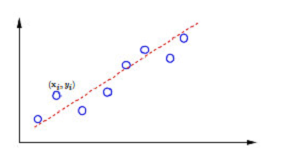
\includegraphics[width=0.5\textwidth]{fig/regressionLineaire1var.png}
	\caption{Régression Linéaire avec une variable}
	\label{fig:image1}
\end{figure}

\textbf{\emph{2 ème cas régression avec plusieurs variables :}}

 Prédire par exemple le prix d'une maison cette fois en fonction de la superficie, du nombre des chambres ,et de l'année de construction

${h}_{\theta}\left(x\right)={\theta }_{0}{x}_{0}+{\theta }_{1}{x}_{1}+{\theta }_{2}{x}_{2}+{\theta }_{3}{x}_{3}+....{\theta }_{n}{x}_{n}$
Dans ce cas notre hypothèse sera en fonction des variables en entrée un plan ou un hyperplan.\\

\textbf{\emph{3 eme cas la regression polynomiale:}}

Dans ce cas au lieu d'utiliser une droite on utilise un polynôme à n dégrée qui es donnée par:

${h}_{\theta}\left(x\right)={\theta }_{0}{x}_{0}+{\theta }_{1}{x}_{1}+{\theta }_{2}{x}_{2}^{2}+{\theta }_{3}{x}_{3}^{3}+....{\theta }_{n}{x}_{n}^{n}$
\begin{figure}[ht]
	\centering
	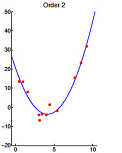
\includegraphics[width=0.5\textwidth]{fig/regressionPlokynome.png}
	\caption{Régression Polynomiale avec un polynôme de degré 2}
	\label{fig:image2}
\end{figure}
le travail restant sera de trouver les paramètres ${\theta }_{i}$ pour notre fonction  ${h}_{\theta}\left(x\right)$ mais comment les trouver?

\subsubsection{Fonction Cout et calcul de L'erreur }
On appelle l'erreur de prédiction , la valeur définie par   :

 $J\left({\theta }_{1},{\theta }_{2},.....{\theta }_{n}\right)=\frac{1}{2m}\sum _{=1}^{m}{\left[{h}_{\theta}\left({x}^{(i)}\right) - {y}^{(i)}\right]}^2$
 avec m : le nombre des nos données d'apprentissage.
 Cette fonction représente l'erreur commise lors de la prédiction avec notre hypothèse par rapport à la valeur exacte.
 Les  ${\theta }_{i}$ sont les valeurs qui minimisent cette erreur sur toutes les données de notre apprentissage.
 
 Il existe différents techniques de minimisation de cette fonction entre autre :
 
  - L'annulation de la dérivée première (trouver les valeurs ${\theta }_{i}$ qui annulent notre dérivée première  ) .Cette méthode à pour inconvénient le fait qu'il convient pas pour les données d'apprentissage avec plusieurs attribues et plusieurs données. 
  
  - une autre méthode c'est la descente du gradient :
  celle ci consiste à effectuer plusieurs itérations sur les valeurs de  ${\theta }_{i}$ jusqu'à trouver celle qui minimise l'erreur (jusqu'à ce qu'il converge vers zéro)
  
  voici l'algorithme utilisée :
\ref{Algo1}
\begin{algorithm}[ht]
	\caption{Algorithme de la descente du gradient }
	\label{Algo1}
	\begin{algorithmic}
		\State ${\theta }_{i} \leftarrow 0$
		\While{J ne converge pas}\Comment{faire pour chaque tuple }
		\State ${\theta }_{i} \leftarrow  {\theta }_{i} - \alpha \frac{\partial }{\partial {{\theta }_{i}}}J\left({\theta }_{1},{\theta }_{2},.....{\theta }_{n}\right)$
		\EndWhile
	\end{algorithmic}
   \end{algorithm}
  
  avec $\alpha$ : learning rate qui est compris entre [0,001;0,1] il sert à réguler notre algorithme
  
  s'il est trop grand $\theta$ ne converge pas
  s'il est trop petit $\theta$ converge après plusieurs itérations. 
  Dans la plupart des cas J converge après un nombre d'itérations élevé
  comme on peut le remarqué sur la figure suivante :
  \begin{figure}[ht]
  	\centering
  	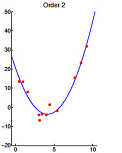
\includegraphics[width=0.5\textwidth]{fig/regressionPlokynome.png}
  	\caption{Variation de J en fonction du nombre des itérations}
  	\label{fig:image3}
  \end{figure}
   
  
  NB :  La Normalisation
  
  Dans la pratique on peut avoir plusieurs données qui ne sont pas dans la même échelle
  
  par ex: on cherche à prédire le prix d'une maison en fonction de la surface ${x}_{1}$ : compris entre 30 -- 400 ${m}^2$, le nombres des chambres ${x}_{2}$ : 1-10,\\
    Nous remarquons que nos 2 variables ne sont pas dans la même intervalle et  cela peut présenter un problème de convergence et ainsi empêcher les ${\theta }_{i}$ de converger rapidement .
   Pour limiter ce problème on effectue une normalisation .Elle consiste à remplacer les ${x}_{i}$ pour chaque tuple par :
   
        ${x}_{j}^{i} =  \frac{{x}_{j}^{i}- {\mu({x}_{j})}}{{\sigma({x}_{j})}}$
        avec : \\
        ${\mu({x}_{j})}$ : la moyenne des termes  ${x}_{j}$ et 
        ${\sigma({x}_{j})}$ : la variance des termes  ${x}_{j}$ 
        \newpage\cleardoublepage	
 \subsection{Régression Logistique  }
 La régression logistique est une technique de classification , elle consiste à appliquer une fonction h sur des éléments ${x}_{1}$ ,${x}_{2}$,${x}_{3}$ .... ${x}_{n}$ en entrée et trouver une sortie \emph{discrète} y. \\
 Cette sortie nous permet de déterminer la classe du tuple , généralement y prend 2 valeurs 0 ou 1 et quelque fois -1  ou 1.\\
 On utilise ce type de classification dans différents cas :

 - Classification des emails : spams ou non spam

 - Transaction en Ligne : Frauduleux ou pas

 - Crédit bancaire : risquant ou non

 - Tumeur : Bénigne ou Maligne

\subsubsection{Représentation de l'hypothèse}
Une première approche serait d'utiliser la régression linéaire avec la fonction ${h}_{\theta}\left(x\right)={\theta }_{0}{x}_{0}+{\theta }_{1}{x}_{1}+{\theta }_{2}{x}_{2}+{\theta }_{3}{x}_{3}+....{\theta }_{n}{x}_{n}$  pour effectuer la classification mais cela peut un problème car ${h}_{\theta}\left(x\right)$ peut prendre des valeur qui sont à l'extérieur de  l'intervalle [0,1].
La meilleur solution serait de trouver une fonction qui ne prend que des valeurs comprises entre 0 et 1 .

Pour les problèmes de classification on utilise la fonction sigmoïde ,elle est définie par :

\begin{center}
	$g(z) =\frac{1}{1+{e}^{-z}}$
\end{center}
Et ainsi notre hypothèse sera :
\begin{center}
	${h}_{\theta}\left(x\right)=g({\theta }^{T}{x})$
\end{center}
Avec ${\theta }^{T}{x}={\theta }_{0}{x}_{0}+{\theta }_{1}{x}_{1}+{\theta }_{2}{x}_{2}+{\theta }_{3}{x}_{3}+....{\theta }_{n}{x}_{n}$.
Voici comment se présente cette fonction :
\begin{figure}[ht]
	\centering
	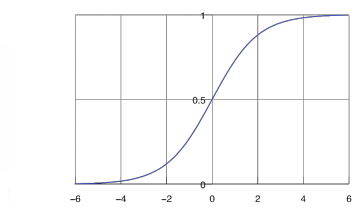
\includegraphics[width=0.5\textwidth]{fig/FonctionSigm.png}
	\caption{Fonction Sigmoïde}
	\label{fig:image4}
\end{figure} \\
On remarque que cette fonction ne prend que des valeurs comprise entre 0 et 1.

En d'autres termes ${h}_{\theta}\left(x\right)$ représente la probabilité que y=1 sur l'entrée  ${x}_{n}$ .
\begin{center}
	${h}_{\theta}\left(x\right)=P(y=1|x;\theta)$
\end{center}
La probabilité que y soit égale à 1 sachant ${x}_{n}$ paramétré par $\theta$.

On l'utilise pour effectuer une classification en supposant que :

- si ${h}_{\theta}\left(x\right)> 0.5 $ la classe prédite est 1.

- si ${h}_{\theta}\left(x\right)< 0.5 $ la classe prédite est 0.

On démontre que :
\begin{center}
	$P(y=1|x;\theta) + P(y=0|x;\theta) = 1 $ et
	
	$P(y=0|x;\theta) = 1-  P(y=1|x;\theta)$
\end{center}
\subsubsection{Frontière de Décision }
Analysons notre fonction $g(z)$ , on remarque qu'il est égale à 0.5 pour z = 0.
Donc si z est positif $g(z)$ sera supérieur à 0.5, dans le cas contraire $g(z)$ sera inférieur à 0.5.
Et ainsi avec notre hypothèse
$h({\theta }^{T}{x}) = 1 $ si  ${\theta }^{T}{x}$ > 0 et 
$h({\theta }^{T}{x}) = 0 $ si  ${\theta }^{T}{x}$ < 0
On comprend qu'a partir du plan  ${\theta }^{T}{x}$ qui divise l'espace en 2 partie on peut prédire la classe de chaque tuple  sans problème .

Cette droite ou hyperplan  s'appelle \emph{\textbf{la frontière de décision }}.
Voici comment elle se présente si on n'a que 2 attributs ${x}_{1}$ et ${x}_{2}$ :
\begin{figure}[ht]
	\centering
	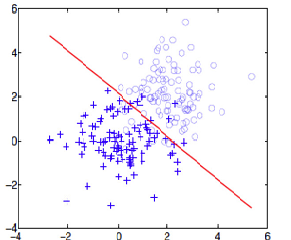
\includegraphics[width=0.5\textwidth]{fig/DecisionBoudary.png}
	\caption{Frontière de décision pour la Régression Logistique à 2 variables}
	\label{fig:image5}
\end{figure}

\subsubsection{La Fonction Coût : Calcul De L'erreur }

On pourrait être tenter d'utiliser la même fonction coût que pour la régression linéaire 

\begin{center}
	 $J\left({\theta }_{1},{\theta }_{2},.....{\theta }_{n}\right)=\frac{1}{2m}\sum _{=1}^{m}{\left[{h}_{\theta}\left({x}^{(i)}\right) - {y}^{(i)}\right]}^2$
\end{center}
Mais cette fonction présente des problèmes de convergence à cause de la non linéarité de la fonction ${h}_{\theta}\left(x\right)$.
Pour ce faire,on définit une nouvelle fonction de l'erreur:

$Err({h}_{\theta}\left(x\right),y) = \left\{\begin{array}{ll}
-\log [1-{h}_{\theta}\left(x\right)], & \mbox{si } y\mbox{=0}   \\
-\log [{h}_{\theta}\left(x\right)], & \mbox{si } y\mbox{=1} 
\end{array}\right.$

\emph{\textbf{Analyse de l'erreur :}}

- si y= 1 et notre fonction ${h}_{\theta}\left(x\right)=1$, alors l'erreur vaut 0 et augmente si  ${h}_{\theta}\left(x\right)$ décroit.

- si y= 0 et notre fonction ${h}_{\theta}\left(x\right)=0$, alors l'erreur vaut 0 et augmente si  ${h}_{\theta}\left(x\right)$ croit . 

On peut facilement le remarquer sur les figures suivantes: \\
\begin{figure}[ht]
	\centering
	\subfloat[cas ou Y =1]{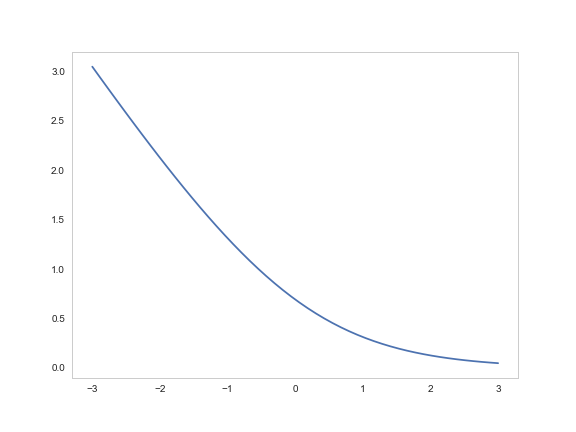
\includegraphics[width=0.4\textwidth]{fig/ErreurRegressionLogistique.png}\label{fig:Image6a}}
	\hfill
	\subfloat[Y = 0]{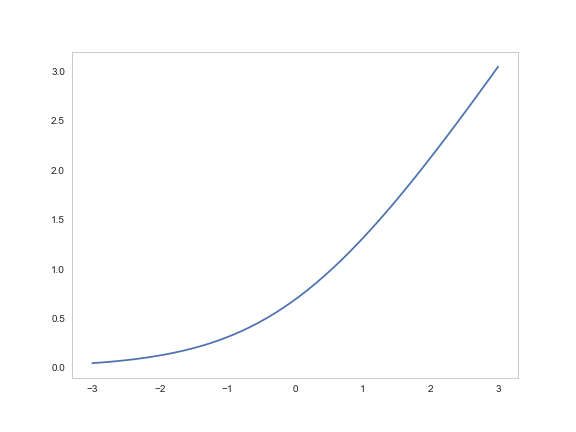
\includegraphics[width=0.4\textwidth]{fig/ErreurRegressionLogistique2.png}\label{fig:Image6b}}
	\hfill
	\caption{Erreur  pour la régression logistique}
\end{figure}
Notre fonction cout peut prendre la forme compacte suivante :
\begin{center}
	$Err({h}_{\theta}\left(x\right),y) = -y\log [{h}_{\theta}\left(x\right)] -(1-y)\log [1-{h}_{\theta}\left(x\right)]$ 
\end{center}	
Et Donc notre Fonction cout pour les $\theta$ sera :
\begin{center}
$J\left({\theta }\right)=\frac{1}{2m}[\sum _{=1}^{m}-{y}^{(i)}\log [{h}_{\theta}\left({x}^{(i)}\right)] -(1-{y}^{(i)})\log [1-{h}_{\theta}\left({x}^{(i)}\right)]]$
\end{center}


Avec ${h}_{\theta}\left(x\right) =\frac{1}{1+{e}^{-{\theta }^{T}{x}}}$

 Pour le minimiser,on recours aux mêmes techniques que pour la régression linéaire et c'est le même algorithme de la descente du gradient qu'on utilise  dans ce cas aussi.
\subsubsection{Régulation : Phénomène de sur-apprentissage}
Nous venons de passer en revue quelques modèles pour  effectuer la régression linéaire ainsi que la classification avec la régression logistique.
Jetons un coup d'œil aux 3 images de la `\figurename{ 7 }  \\
\begin{figure}[ht]
	\centering
	\subfloat[${h}_{\theta}\left(x\right)={\theta }_{0}+{\theta }_{1}x$]{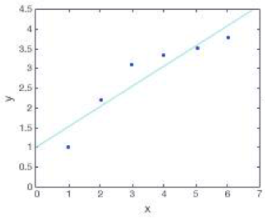
\includegraphics[width=0.4\textwidth]{fig/Overfiitting1.png}\label{fig:Image7a}}
	\hfill
	\subfloat[${h}_{\theta}\left(x\right)={\theta }_{0}+{\theta }_{1}x+{\theta }_{2}{x}^{2}$]{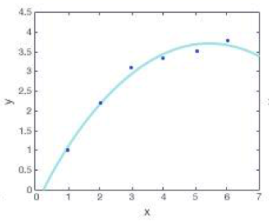
\includegraphics[width=0.4\textwidth]{fig/Overfiitting2.png}\label{fig:Image7b}}
	\hfill
	\subfloat[${h}_{\theta}\left(x\right)={\theta }_{0}+{\theta }_{1}x+{\theta }_{2}{x}^{2}+{\theta }_{3}{x}^{3}+{\theta }_{4}{x}^{4}$]{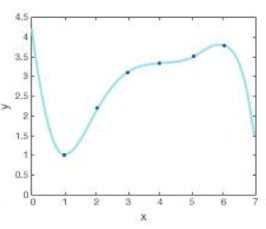
\includegraphics[width=0.4\textwidth]{fig/Overfiitting3.png}\label{fig:Image7c}}
	\caption{a: Sous-apprentissage et c : Sur-apprentissage avec la régression linéaire}
\end{figure}
A la première figure (a) : avons la régression linéaire comme hypothèse  mais on remarque que cela n'est pas un bon modèle de prédiction car dans ce cas l'erreur est trop grande.on parle de \emph{sous-apprentissage ou Underfitting}.
A la deuxième figure notre hypothèse c'est un polynôme du second dégrée le modèle convient bien à notre ensemble d'apprentissage et dans ce cas l'erreur est moins élevée.
Par contre sur la troisième cas l'hypothèse c'est un polynôme du quatrième dégrée qui convient parfaitement à notre ensemble d'apprentissage et l'erreur est nulle, mais c'est modèle n'est pas bon  car il  convient parfaitement sur notre ensemble d'apprentissage et n'est pas adaptable aux nouvelles données, elle n'est pas une solution générale.Dans ce cas on parle de \emph{Sur-Apprentissage ou Overfitting } .

On remarque ce même phénomène avec la régression logistique .

\begin{figure}[H]
	\centering
	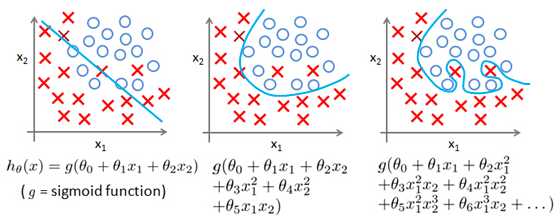
\includegraphics[width=0.5\textwidth]{fig/OverfiittingLogistic.png}
	\caption{Overfitting et Underfitting avec la régression logistique }
	\label{fig:image8}
\end{figure}
\subsubsection{Solutions aux problèmes de sur apprentissage }
Signalons qu'une des cause de ce phénomène c'est le fait d'avoir peut des données avec plusieurs attributs .

Dans ce cas la première de solution consisterait à réduire le nombre des attribues , choisir celle qu'on doit retenir et laisser les autres,mais cette approche possède un inconvénient car on risquerait de perdre l'information apportée par ces attributs et cela pénaliserait notre modèle .

La seconde solution est celle qu'on appelle la \emph{La régularisation } elle consiste à garde tous les attributs mais réduire l'ampleur des paramètres  $\theta$ dans le calcul de l'erreur . On remarque que cette technique fonctionne très bien lorsqu'on dispose de plusieurs attributs qui contribue à la prédiction de la valeur y.
Ainsi notre fonction de cout pour le calcul de l'erreur de la régression linéaire sera :

\begin{center}
	$J\left({\theta }_{1},{\theta }_{2},.....{\theta }_{n}\right)=\frac{1}{2m}[\sum _{=1}^{m}{\left[{h}_{\theta}\left({x}^{(i)}\right) - {y}^{(i)}\right]}^{2} + {\lambda} \sum _{=1}^{n}{{\theta}_{j}^{2}}]$
\end{center}
Et Pour la régression logistique elle sera :

\begin{center}
	$J\left({\theta }\right)=\frac{1}{2m}[\sum _{=1}^{m}-{y}^{(i)}\log [{h}_{\theta}\left({x}^{(i)}\right)] -(1-{y}^{(i)})\log [1-{h}_{\theta}\left({x}^{(i)}\right)] + {\lambda} \sum _{=1}^{n}{{\theta}_{j}^{2}}]$
\end{center}

Avec $\lambda$ le facteur de régularisation. 
C'est cette nouvelle fonction cout qu'on utilise pour l'algorithme de la descente du gradient régularisé.\\ 
\newpage\cleardoublepage
\subsection{Le Réseaux des Neurones }
Pourquoi avons nous besoins du réseau des neurones? 
Supposons que nous avons un problème complexe de classification, la première approche serait d'utiliser la classification logistique avec un polynôme de plusieurs termes :

- cela conviendrait pour problème avec 1, ou 2 attribut.

- supposons maintenant que nous avons des  tuples avec plus de 1000 attributs ,

Ex: On veut prédire la chance d'une maison d'être vendu dans 6 mois  :
- Plusieurs facteurs entrent en jeu ,à peut près plus de 100 , on aura un polynôme avec les termes suivants (${x}_{1}^{2},{x}_{1}{x}_{2},{x}_{1}{x}_{3},{x}_{1}{x}_{4},...{x}_{1}{x}_{100}$),
on aura a peut près 5000 termes et ce nombre augmentera énormément si on choisi de considérer les 3 ème degré.
La régression logistique n'est pas vraiment approprié pour des problèmes de classification des données avec plusieurs attributs .

Par exemple dans le cas de la vision artificielle ou n peut aller de 2500 à 50000000  attributs.
On remarque bien qu'une simple régression logistique n'est pas approprié pour ce cas.

\subsubsection{Les Neurones et le cerveau\cite{NNBook}}

Une des motivations qui ont poussé les scientifique à créer le réseaux des neurones c'est celui de répliquer le fonctionnement du cerveau humain .
En effet le cerveaux humain dispose d'une capacité énorme d'apprentissage il s'apprend lui même comment apprendre et peut apprendre de n'importe quelle source des données,il  contient environ 100 milliards de neurones.
Voici à quoi ressemble à quoi ressemble un neurone dans le cerveau:
\begin{figure}[ht]
	\centering
	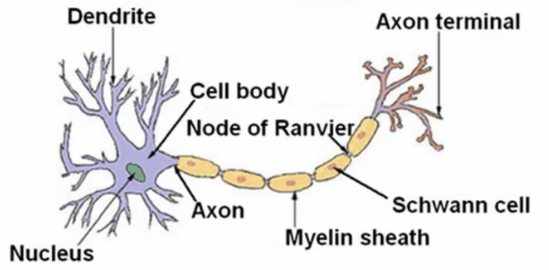
\includegraphics[width=0.5\textwidth]{fig/Neurone.png}
	\caption{Un Neurone Naturel}
	\label{fig:image9}
\end{figure}

Les neurones reçoivent les signaux (impulsions électriques) par des extensions très ramifiées de leur corps cellulaire (les dendrites) et envoient l'information par de longs prolongements (les axones). Les impulsions électriques sont régénérées pendant le parcours le long de l'axone. La durée de chaque impulsion est de l'ordre d'1 ms et son amplitude d'environ 100 mvolts.
Les contacts entre deux neurones, de l'axone à une dendrite, se font par l'intermédiaire des synapses. Lorsqu'un potentiel d'action atteint la terminaison d'un axone, des neuromédiateurs sont libérés et se lient à des récepteurs post-synaptiques présents sur les dendrites. L'effet peut être excitateur ou inhibiteur.
Chaque neurone intègre en permanence jusqu'à un millier de signaux synaptiques. Ces signaux n'opèrent pas de manière linéaire (effet de seuil).

\subsubsection{Représentation d'un Neurone Artificiel }
On pourrait définir un neurone  ou perceptrons comme étant une unité de traitement qui reçoit des données en entrée sous forme vectorielle et produit une sortie réelle , cette sortie est fonction des entrées et des poids de connexions.

Il se caractérise par :

- les signaux en entrée  ${x}_{1},{x}_{2},....,{x}_{n}$ ,

 il est toujours préférable d'ajouter le biais ${x}_{0}$ qui est égale à 1.,

- les coefficients synaptiques ou poids des connexions ${\theta}_{i0},{\theta}_{i1},....{\theta}_{in}$,

- Une Fonction d'activation ${h}_{\theta}(x)$,

- l'état interne d'activation $a={h}_{\theta}(x)$

\begin{figure}[ht]
	\centering
	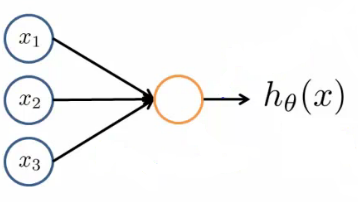
\includegraphics[width=0.5\textwidth]{fig/SimpleANN.png}
	\caption{un Perceptron  ou Unité de traitement}
	\label{fig:image10}
\end{figure}

D'une façon plus générale un  réseau des neurones est un ensemble de plusieurs neurones liés entre eux pour effectuer un calcul se compose :

- D'une couche d'entré ou activation layer 

- D'une couche de sortie ou output layer  

- D'une ou plusieurs couches intermédiaires ou hidden layers .

\begin{figure}[ht]
	\centering
	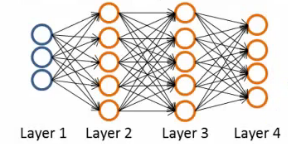
\includegraphics[width=0.5\textwidth]{fig/FullNeural.png}
	\caption{un réseau des neurones complets avec 2 hidden layers }
	\label{fig:image11}
\end{figure}

Chaque couche dispose des perceptrons ou unités d'activation.\\
On note :

 - ${a}_{i}^{j}$ : l'unité d'activation i de la couche j
 
 
 - ${\theta}^{l}$ : matrice des poids de connexions contrôlant le passage de la couche l à couche l+1.\\
 La matrice ${\theta}^{l}$ est constituée des termes ${\theta}_{ij}$ avec:
 
 - i l'indice de l'unité de la couche de destination
 
 - j l'indice de l'unité de la couche d'origine .\\
  Donc ${\theta}_{12}$ représente le poids de passage de l'unité 2 de la couche d'origine a l'unité 1 de la couche de destination.\\
 Regardons encore une fois l'image suivante :
\begin{figure}[ht]
 	\centering
 	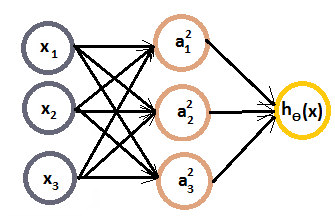
\includegraphics[width=0.5\textwidth]{fig/NeuralNtwork2.png}
 	\caption{Réseaux des neurones avec des unités d'activation }
 	\label{fig:image12}
\end{figure}\\
 Nous avons : \\
 ${a}_{1}^{(2) }= g({\theta}_{10}^{(1)}{x}_{0} + {\theta}_{11}^{(1)}{x}_{1} + {\theta}_{12}^{(1)}{x}_{2} + {\theta}_{13}^{(1)}{x}_{3})$ \\
 ${a}_{2}^{(2) }= g({\theta}_{20}^{(1)}{x}_{0} + {\theta}_{21}^{(1)}{x}_{1} + {\theta}_{22}^{(1)}{x}_{2} + {\theta}_{23}^{(1)}{x}_{3})$ \\
 ${a}_{3}^{(2) }= g({\theta}_{30}^{(1)}{x}_{0} + {\theta}_{31}^{(1)}{x}_{1} + {\theta}_{32}^{(1)}{x}_{2} + {\theta}_{33}^{(1)}{x}_{3})$ \\
 ${h}_{\theta}(x) ={a}_{1}^{(3) }= g({\theta}_{10}^{(2)}{a}_{0}^{(2)} + {\theta}_{11}^{(2)}{a}_{1}^{(2)} + {\theta}_{12}^{(2)}{a}_{2}^{(2)} + {\theta}_{13}^{(2)}{a}_{3}^{(2)})$ \\
 
 Chaque unité d'activation de la couche l+1 est obtenue en appliquant la fonction g (une sigmoïde ) aux à la combinaison linéaire des unités de la couche précédente avec les éléments de la matrice ${\theta}^{l}$. \\
 \subsubsection{Apprentissage par Réseau des neurones }
 Le réseau des neurones est un des plus puissant algorithme d'apprentissage ,
 il cherche à trouver les paramètres du modèle d'apprentissage uniquement à partir de l'ensemble d'apprentissage .\\
 Voici notre configuration :
 
 - Notre ensemble d'apprentissage est : {$({x}^{1},{y}^{1}),({x}^{2},{y}^{2}),({x}^{3},{y}^{3}),....({x}^{n},{y}^{m})$}
 
 - L nombre des couche de notre réseau . Pour notre cas L=4
 
 -${s}_{l}$ nombre des unités dans la couche l\\
 Donc en se référant à la \figurename{ 11} On remarque que :
 
 - L= 4
 
 - ${s}_{1} = 3$
 
 - ${s}_{2} = 5$
 
 - ${s}_{3} = 5$
 
 - ${s}_{4} = 4$
 
 Avec le réseaux des neurones on peut faire aussi bien des classification binaires que des classifications avec plusieurs classe.\\
 Pour la classification binaire la couche de sortie ne comprend qu'une seule unité k = 1 avec k le nombre des unités de la couche  de sortie.\\
 Pour une classification multi-classe k prend des valeurs supérieurs à 3,\\ la sortie  $y \in {\LARGE R}^{K} $  Pour 3 classes ${y}^{1} = [1,0,0]$ , ${y}^{2} = [0,1,0]$ , ${y}^{3} = [0,0,1]$; 
 \subsubsection{Fonction Cout}
 
 Rappelons que pour la régression logistique la fonction cout régularisée est la suivante :
 
\begin{center}
 	$J\left({\theta }\right)=\frac{1}{2m}[\sum _{i=1}^{m}-{y}^{(i)}\log [{h}_{\theta}\left({x}^{(i)}\right)] -(1-{y}^{(i)})\log [1-{h}_{\theta}\left({x}^{(i)}\right)] + {\lambda} \sum _{j=1}^{n}{{\theta}_{j}^{2}}]$
\end{center} 
 Pour le réseau des neurones la  fonction cout n'est que la généralisation de celui de la régression logistique mais au lieu d'une sortie nous avons K sorties .
 
 ${h}_{\theta}\left(x\right) \in {\LARGE R}^{k} $  et 
 $({h}_{\theta}\left(x\right))_{k} = {k}^{eme} $  sortie 
 
 
  	$J\left({\theta }\right)=\frac{1}{2m}[\sum _{i=1}^{m}\sum _{k=1}^{K}-{y}_{k}^{(i)}\log [({h}_{\theta}\left({x}^{(i)}\right))_{k}] -(1-{y}_{k}^{(i)})\log [1-({h}_{\theta}\left({x}^{(i)}\right))_{k}] + {\lambda} \sum _{l=1}^{L-1}\sum _{i=1}^{{s}_{l}}\sum _{j=1}^{{s}_{l+1}}{({\theta}_{ji}^{(l)})^{2}}]$ \\

Une fois la fonction cout connu le reste du travail consiste à entrainer notre réseau , donc de  trouver :

- la valeur des unités d'activation ${a}^{l}$ pour chaque couche 

- Ainsi que celles de ${\theta}_{ji}^{(l)}$ qui minimisent la fonction cout .

\subsubsection{Calcul des Valeurs des unités d'activation \emph{Forward propagation}}

Cette technique est celle qui permet de calculer  de calculer les valeur des unités d'activation du réseau des neurones en partant de la couche d'entrée et propagé ces valeurs jusqu'à   la couche de sortie d'où le nom de \emph{Forward propagation}.\\
Nous avons déjà établie que : \\
- ${a}_{1}^{(2) }= g({\theta}_{10}^{(1)}{x}_{0} + {\theta}_{11}^{(1)}{x}_{1} + {\theta}_{12}^{(1)}{x}_{2} + {\theta}_{13}^{(1)}{x}_{3})$ \\
- ${a}_{2}^{(2) }= g({\theta}_{20}^{(1)}{x}_{0} + {\theta}_{21}^{(1)}{x}_{1} + {\theta}_{22}^{(1)}{x}_{2} + {\theta}_{23}^{(1)}{x}_{3})$ \\
- ${a}_{3}^{(2) }= g({\theta}_{30}^{(1)}{x}_{0} + {\theta}_{31}^{(1)}{x}_{1} + {\theta}_{32}^{(1)}{x}_{2} + {\theta}_{33}^{(1)}{x}_{3})$ \\
on définie : \\
 $ {z}_{1}^{2} = {\theta}_{10}^{(1)}{x}_{0} + {\theta}_{11}^{(1)}{x}_{1} + {\theta}_{12}^{(1)}{x}_{2} + {\theta}_{13}^{(1)}{x}_{3}$ et cela veut dire que :\\
 ${a}_{1}^{(2) } = g({z}_{1}^{2} )$ \\
 On peut ainsi définir les termes  ${z}_{2}^{2}$ ,et ${z}_{3}^{2}$ qui sont les unités d'activation de la couche 2.\\
 En utilisant les matrices  nous pouvons écrire :
 
 ${z}^{(2)} = 
\begin{bmatrix}
 {z}_{1}^{(2)}\\ 
 {z}_{2}^{(2)} \\ 
 {z}_{3}^{(2)}
\end{bmatrix} $  pour la 2ème couche et l'entrée peut être noté $x = 
\begin{bmatrix}
 1\\ 
 {x}_{1} \\ 
 {x}_{2} \\
 {x}_{3} 
\end{bmatrix} $ \\
Ainsi ${z}^{(2)} = {\theta}^{(1)}x$ et ${a}^{(2)}=g({z}^{(2)})$ \\
Pour la troisième couche écrit :   ${z}^{(3)} = {\theta}^{(2)}{a}^{2}$ et ${a}^{(3)}=g({z}^{(3)})$   et ainsi de suite jusqu'à la couche de sortie .\\
D'une façon générale on écrit : ${z}^{(l)} = {\theta}^{(l-1)}{a}^{l-1}$ et ${a}^{(l)}=g({z}^{(l)})$ pour toutes les couches du réseau .

\subsubsection{Minimisation de la fonction de cout : back propagation }
Pour minimiser la fonction cout on doit calculer ses dérivées partielle par rapport aux éléments ${\theta}_{ji}^{(l)}$ ce qui n'est pas une tache facile .
Le but est de trouver les ${\theta}_{ji}^{(l)}$ qui minimisent la fonction cout.
On veut calculer $\frac{\partial }{\partial {\theta}_{ji}^{(l)} }J\left({\theta }\right)$ \\
Pour calculer les dérivées partielles on utilise la technique qu'on appelle \emph{back propagation } ou \emph{rétro-propagation du gradient  } ,c'est une méthode qui permet de calculer le gradient de l'erreur pour chaque neurone d'un réseau de neurones, de la dernière couche vers la première.\\
Notons ${\delta}_{j}^{l}$ : l'erreur à l'unité j de la couche l. \\
- Pour la 4eme couche  cette erreur n'est que la différence entre la valeur exacte et la valeur calculé par notre réseau des neurones.

D'ou :  ${\delta}_{j}^{4} = {a}_{j}^{4} - y_j$ \\
\begin{comment}
\emph{Démonstration }:
 Si on ne considère qu'un seul élément dans l'ensemble d'apprentissage et on ignore le terme de régularisation la fonction cout  de la 4 eme couche sera :
 
  $J\left({\theta }\right)= {y}_{(i)}\log ({a}^{4}) + (1-{y}_{(i)})\log (1-({a}^{4})) $ avec ${a}^{(4)}=g({z}^{(4)})$ \\
  ${\delta}_{j}^{4} = \frac{\partial J\left({\theta }\right) }{\partial {z}_{j}^{(4)} }$ \\
  = $\frac{\partial [{y}_{(i)}\log (g({z}^{(4)})) + (1-{y}_{(i)})\log (1-(g({z}^{(4)}))) ]}{\partial {z}_{j}^{(4)} }$ \\
  =${y}_{(i)}\frac {\partial g({z}^{(4)})  } {\partial {z}_{j}^{(4)} } \frac{1}{g({z}^{(4)}) } + (1-{y}_{(i)}) \frac {\partial( 1- g({z}^{(4)}))  } {\partial {z}_{j}^{(4)}} \frac{1}{1-g({z}^{(4)}) } $\\
  Avec $g(z) =\frac{1}{1+{e}^{-z}}$ et on démontre que $g^{'}(z) = (1-g(z))g(z)$ \\
  =${y}_{(i)} ({1-g({z}^{(4)}) } )g({z}^{(4)}) \frac{1}{g({z}^{(4)}) } -  (1-{y}_{(i)}) ({1-g({z}^{(4)}) } )g({z}^{(4)}) \frac{1}{1-g({z}^{(4)}) } $ \\
  =${y}_{(i)} ({1-g({z}^{(4)}) } ) -  (1-{y}_{(i)})g({z}^{(4)})  $ \\
  =${y}_{(i)} - g({z}^{(4)})$ \\
 D'ou ${\delta}_{j}^{4} = {y}_{(i)} - g({z}^{(4)}) $ \\
Avec ${\delta}_{j}^{4}$ on calcul l'erreur pour l'unité j  de la 3ème couche qui est ${\delta}_{j}^{3}$ \\
 ${\delta}_{j}^{3} = \frac{\partial J\left({\theta }\right) }{\partial {z}_{j}^{(3)} }$ \\
 ${\delta}_{j}^{3} = \frac{\partial J\left({\theta }\right) }{\partial {z}_{j}^{(4)} } \frac{\partial {z}_{j}^{(4)} }{\partial {z}_{j}^{(3)} }$ \\
 ${\delta}_{j}^{3} = {\delta}_{j}^{4} \frac{\partial {z}_{j}^{(4)} }{\partial {z}_{j}^{(3)} }$  or ${z}_{j}^{(4)} = {\theta}_{ij}^{(3)}{a}^{3}$ \\
 ${\delta}_{j}^{3} = {\delta}_{j}^{4} \frac{\partial ({\theta}_{ij}^{(3)}{a}^{3}) }{\partial {z}_{j}^{(3)} }$ \\
 ${\delta}_{j}^{3} = {\delta}_{j}^{4}  {\theta}_{ij}^{(3)} \frac{\partial ({a}^{3}) }{\partial {z}_{j}^{(3)} }$  or ${a}_{j}^{(3)}=g({z}_{j}^{(3)})$ Donc ,\\
 ${\delta}_{j}^{3} = {\delta}_{j}^{4}  {\theta}_{ij}^{(3)} \frac{\partial g({z}^{(3)}) }{\partial {z}_{j}^{(3)} }$ , ce qui nous donne \\
 ${\delta}_{j}^{3} = {\delta}_{j}^{4}  {\theta}_{ij}^{(3)}  (1- g({z}_{j}^{(3)}))g({z}_{j}^{(3)}) $  ou encore \\
 ${\delta}_{j}^{3} = {\delta}_{j}^{4}  {\theta}_{ij}^{(3)}  (1- {a}_{j}^{(3)}){a}_{j}^{(3)}$ \\
 
 On peut aussi calculer : $ \frac{\partial J\left({\theta }\right) }{\partial {\theta}_{ij}^{(3)} }$  \\
 $ \frac{\partial J\left({\theta }\right) }{\partial {\theta}_{ij}^{(3)} } =
 \frac{\partial J\left({\theta }\right) }{\partial {z}_{j}^{(4)} } \frac{\partial {z}_{j}^{(4)} }{\partial  {\theta}_{ij}^{(3)} }
 $ \\
 $ \frac{\partial J\left({\theta }\right) }{\partial {\theta}_{ij}^{(3)} }= {\delta}_{j}^{4} . {a}_{j}^{3} $\\
 
 De la même faon calcul l'erreur de la couche 2 et on peut prouver que c'est égale à :
 ${\delta}_{j}^{2} = {\delta}_{j}^{3}  {\theta}_{ij}^{(2)}  (1- {a}_{j}^{(2)}){a}_{j}^{(2)}$  et \\ 
 $ \frac{\partial J\left({\theta }\right) }{\partial {\theta}_{ij}^{(2)} }= {\delta}_{j}^{3} . {a}_{j}^{2} $\\
 
 Notons qu'il n'y a pas de  ${\delta}_{j}^{1}$ car on est à l'entrée .
 
 D'une façon générale , on définit l'erreur de l'unité j de la couche l comme : \\
 ${\delta}_{j}^{l} = {\delta}_{j}^{l+1}  {\theta}_{ij}^{(l)}  (1- {a}_{j}^{(l)}){a}_{j}^{(l)}$ et \\
 $ \frac{\partial J\left({\theta }\right) }{\partial {\theta}_{ij}^{(l)} }= {\delta}_{j}^{l+1} . {a}_{j}^{l} $\\
 Et d'une façon matricielle , l'erreur des unitéq de la couche l est définie par  : \\
  ${\delta}^{L} = {a}^{(L)} - {y}^{(i)} $ pour la dernière couche \\ 
  ${\delta}^{l} =({\theta}^{(l)})^{T} {\delta}^{l+1}.*({a}^{(l)}.*(1- {a}^{(l)}))$  à partir de la couche l-1 et \\
  $ \frac{\partial J\left({\theta }\right) }{\partial {\theta}^{(l)} }= {\delta}^{l+1} . {a}^{l} $\\
\end{comment}
 Pour calculer l'erreur de la couche l on utilise la couche suivante l+1 d'ou le  non de \emph{rétro-propagation du gradient  }
 Ainsi l'algorithme d'entrainement de notre algorithme sera le suivant :
 \ref{Algo2}
\begin{algorithm}
	\caption{Algorithme de la rétro-propagation du gradient }
\begin{algorithmic}
\Require $({x}^{1},{y}^{1}),({x}^{2},{y}^{2}),....({x}^{n},{y}^{m})$
\For{$ i=1,2 ....,{s}_{l+1},j=1,2,....{s}_{l};l=1,2,....L$ }  
\State ${\theta}_{ij}^{(l)}\gets 0$ \Comment{initialsation des valeurs des $\theta $ pour chaque couche à Zero }
   \EndFor
 \ForAll{tuple dans l'ensemble d'apprentissage } 
 \State ${a}^{1} \gets  {x}^{i}$ \Comment {initialisation de la premiere couche avec les valeurs de l'entréé}
 \Repeat
 \For{L =2,3.....L } \Comment{Forward Propagation}
 \State  ${z}^{(l)} \gets {\theta}^{(l-1)}{a}^{l-1}$ 
 \State ${a}^{(l)} \gets g({z}^{(l)})$
 
  \EndFor
\State  ${\delta}^{L} \gets {a}^{(L)} - {y}^{(i)} $ \Comment {pour la dernière couche}
\For {L =L-1,....,2,1 } \Comment {Backward Propagation }
\State ${\delta}^{l} \gets ({\theta}^{(l)})^{T} {\delta}^{l+1}.*({a}^{(l)}.*(1- {a}^{(l)}))$  \
\State $ \frac{\partial J\left({\theta }\right) }{\partial {\theta}^{(l)} } \gets  {\delta}^{l+1} . ({a}^{l})^T $
\State ${\theta}^{(l)}\gets {\theta}^{(l)} +  \frac{\partial J\left({\theta }\right) }{\partial {\theta}^{(l)} }  $  \Comment {Descente d gradient }
\EndFor
\Until{$ J\left({\theta }\right)   $ converge vers 0 }
\If{$j \neq 0$} 
\State ${D}^{l} \gets \dfrac{1}{2m}  {\theta}^{(l)} + \lambda {\theta}^{(l) } $ \Comment {Regularisation }
\Else 
\State ${D}^{l} \gets \dfrac{1}{2m}  {\theta}^{(l)}$ \Comment {Au cas ou il n'ya pas de regularisation }
\EndIf
  \EndFor
\end{algorithmic}
\end{algorithm}
\newpage\cleardoublepage
\subsection{Support Vector Machine - SVM \cite{SVm1} }
Support Vector Machine est un classeur discriminant qui est défini par un hyperplan , étant donné un ensemble d'apprentissage l'algorithme de SVM permet de trouver un hyperplan qui va catégoriser les éléments de l'ensemble et d'autres nouveaux éléments en maximisant la marge entre les élements de l'ensemble d'apprentissage  à la manière de la frontière de décision pour la régression logistique. On peut dire que SVN est une amélioration de la régression logistique .
\subsubsection{Données Séparables linéairement }
Si nous considérons le même problème de classification binaire que celui de la régression logistique sauf que les label de nos classe ici sont 1 et -1 au lieu de 0 et 1 donc ici y $\in$ \{-1,1\} , on constate que nous avons un large variétés des choix pour notre frontière de décision  comme on peut le voir à la figure ci dessous :
\begin{figure}[ht]
	\centering
	\subfloat[]{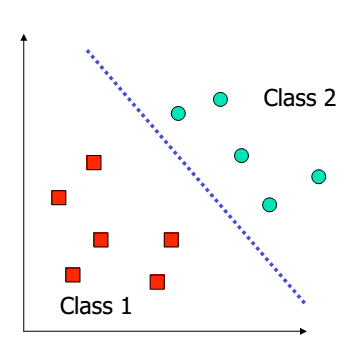
\includegraphics[width=0.3\textwidth]{fig/SVNDecisionBoundary1.png}\label{fig:Image13a}}
	\hfill
	\subfloat[]{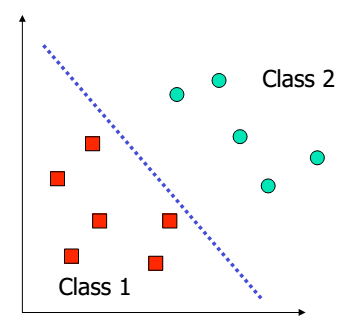
\includegraphics[width=0.3\textwidth]{fig/SVNDecisionBoundary2.png}\label{fig:Image13b}}
	\hfill
	\subfloat[]{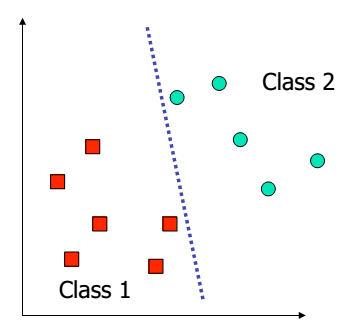
\includegraphics[width=0.3\textwidth]{fig/SVNDecisionBoundary3.png}\label{fig:Image13c}}
	\caption{Différentes frontières de décision possibles }
\end{figure}
Nous remarquons que toutes ces frontières des décisions conviennent pour notre ensemble d'apprentissage.\\ Mais comment alors choisir la bonne?? celle qui est optimale?\\
Remarquons que pour mieux généraliser les données la meilleur  frontière de décision est celle qui doit être le plus éloigné que possible des nos données .  
Le but de SVM revient à trouver cette hyperplan qui constituerai notre frontière de décision.
\paragraph{Représentation de l'hypothèse }
Rappelons que pour la régression logistique notre hypothèse s'écrivait de la manière suivante :
\begin{center}
	${h}_{\theta}\left(x\right)=g({\theta }^{T}{x})$
\end{center} Avec $g(z)$ étant définit comme la fonction sigmoïde.\\
On a aussi fait remarquer qu'on utilise l'équation de la frontière  de décision qui est $({\theta }^{T}{x})$ pour effectuer la classification.
et de la on déduit que les données de la classe positif vérifierons l'équation ${\theta }^{T}{x} > 1$ et les autres ${\theta }^{T}{x} <-1$ .\\
Ainsi la limite de la classe positif est l'hyperplan d'équation  ${\theta }^{T}{x} = 1$  et celle des négatifs est ${\theta }^{T}{x} =-1$ si on tient compte de b comme distance avec l'origine ces droites s'écriront 
${\theta }^{T}{x} + b = 1$  et ${\theta }^{T}{x} + b=- 1$ .
 \begin{figure}[ht]
 	\centering
 	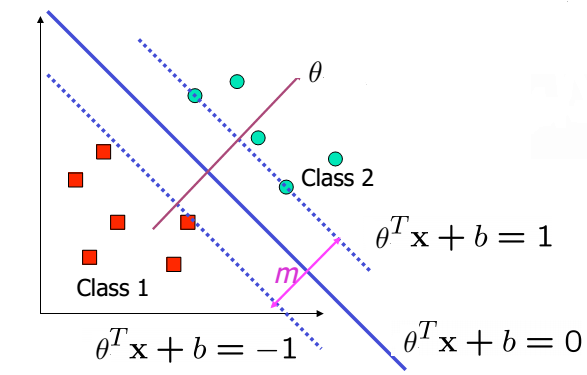
\includegraphics[width=0.5\textwidth]{fig/SVN2D.png}
 	\caption{Problème de SVM en 2 dimensions  }
 	\label{fig:image14}
 \end{figure}\\
Ainsi le but de SVM serait de trouver l'hyperplan qui maximise la marge ou la distance  entre ces 2  hyperplans, et d'après la géométrie analytique cette distance se calcule de la manière suivante $d =\frac{2}{||\theta||}$
Notre problème se formulerait de la manière suivante :
\begin{center}
	$ \left\{\begin{array}{ll}
	max  \frac{2}{||\theta||} ,&  \\
     \mbox{Avec } {\theta }^{T}{x} + b > 1	, & \mbox{si } y\mbox{=1} \\
          \mbox{et  } {\theta }^{T}{x} + b < -1	, & \mbox{si } y\mbox{=-1} 
	\end{array}\right.$
\end{center}
Or maximiser $\frac{2}{||\theta||}$ revient simplement à minimiser $ \frac{1}{2}\theta$
et nos 2 conditions peuvent se combiner en une seule qui est ${y}_{i}({\theta }^{T}{x}_{i} + b )\geq 1 $  $\forall i $ \\
Ainsi le problème à résoudre devient le suivant :
\begin{center}
	$ \left\{\begin{array}{ll}
	min  \frac{1}{2} {||\theta||} ,&  \\
	{y}_{i}({\theta }^{T}{x}_{i} + b )\geq 1, &  \mbox{ $ \forall i$ } \\
	\end{array}\right.$
\end{center}
Ceci n'est rien d'autre qu'un problème d'optimisation sous contrainte, pour le résoudre on utilise la méthode de Lagrange .\\
Elle consiste à cherche le lagrangien de notre problème et égaliser son gradient à zéro.\\
le lagrangien est donné par : 
\begin{center}
 $ {\Large L} = \frac{1}{2} {\theta}^{T} \theta + \sum _{i=1}^{m}{\alpha}_{i}(1-{y}_{i}({\theta }^{T}{x}_{i} + b ))$
 , car  $|| {\theta}||^{2} = {\theta}^{T} \theta $ 
\end{center} 
et ${\nabla }{L}=0$ \\
Ce qui nous donne : \\
$\frac{\partial L}{\partial {\theta}} =  \theta -  \sum _{i=1}^{m}{\alpha}_{i}{y}_{i}{x}_{i} =0$   ce qui donne  $\theta =  \sum _{i=1}^{m}{\alpha}_{i}{y}_{i}{x}_{i}$\\
$\frac{\partial L}{\partial {b }} =0 $ nous donne $\sum _{i=1}^{m}{\alpha}_{i}{y}_{i}=0 $ \\
En mettant ces 2 expressions des L on obtient : \\
${\Large L} =\frac{-1}{2} \sum _{i=1}^{m} \sum _{i=j}^{m} {\alpha}_{i}{\alpha}_{j}{y}_{i}{y}_{j} {X}_{i}^{T} . {{X}_{j}}+ \sum _{i=1}^{m} {\alpha}{i} $ \\
  ,qui n'est qu'une fonction de ${\alpha}_{i}$ \\
Il est connu sous le nom d'un problème de dualité car si on connait ${\alpha}_{i}$ on connait ${\theta}$  
L doit être maximise maintenant , ainsi notre problème de dualité s'écrira :\\
\begin{center}
	$ \left\{\begin{array}{ll}
	max \sum _{i=1}^{m} {\alpha}{i} -  \frac{1}{2} \sum _{i=1}^{m} \sum _{i=j}^{m} {\alpha}_{i}{\alpha}_{j}{y}_{i}{y}_{j} {X}_{i}^{T} . {{X}_{j}},&  \\
	\mbox{Avec } \sum _{i=1}^{m}{\alpha}_{i}{y}_{i}=0 , & \\
	\mbox{et }{\alpha}_{i} \ge 0 
	\end{array}\right.$
\end{center}
Avant de s'attaquer à la résolution de ce problème remarquons quelque éléments intéressants qu'il présente :\\
-  la grande partie des valeurs de ${\alpha}_{i}$ sont nulles et  aux    valeurs non nulles correspondent des ${x}_{i}$ qu'on appelle support Vector.\\
-  Pour prédire la classe d'un  nouveaux élément z nous avons qu'a vérifier s'il se place au dessus ou en dessous de notre frontière de décision qui est donnée par ${\theta }^{T}{z} + b =  \sum _{i=1}^{m}{\alpha}_{i}{y}_{i}({X}^{T}_{i}.Z) $. \\
- Mais aussi il présente l'avantage que l'algorithme comprend le produit scalaire des tuples d'entrés , cet avantage sera utilisé lorsqu'on va traiter des frontières de  décisions non linéairement séparable.
\subsubsection{Données non Séparables linéairement : Notion de Kernel  \cite{SVm2}}
Dans la plupart des cas surtout dans la pratique les données ne peuvent pas toujours être classer avec une droite ou un hyperplan comme on peut le voir à la \figurename{15} :
 \begin{figure}[ht]
 	\centering
 	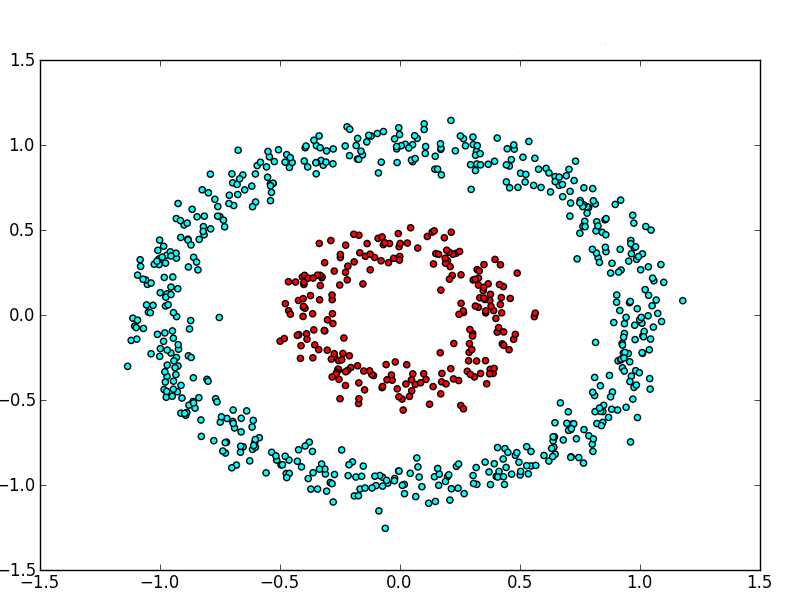
\includegraphics[width=0.5\textwidth]{fig/NonLinearDecisionBoudary.png}
 	\caption{Données non séparable linéairement  }
 	\label{fig:image15}
 \end{figure}\\
 Une propriété stipule que les données qui ne sont pas linéairement séparable dans un espace de dimension n le seront dans un espace de dimension m avec $m \ge n$ \cite{8}. il suffit juste de faire un mapping des tuples ${x}_{i}$  dans ${R}^{n}$ vers ${R}^{m}$ en utilisant une fonction $\phi(x)$. Voyons un exemple à la \figurename{16}\\
  \begin{figure}[ht]
  	\centering
  	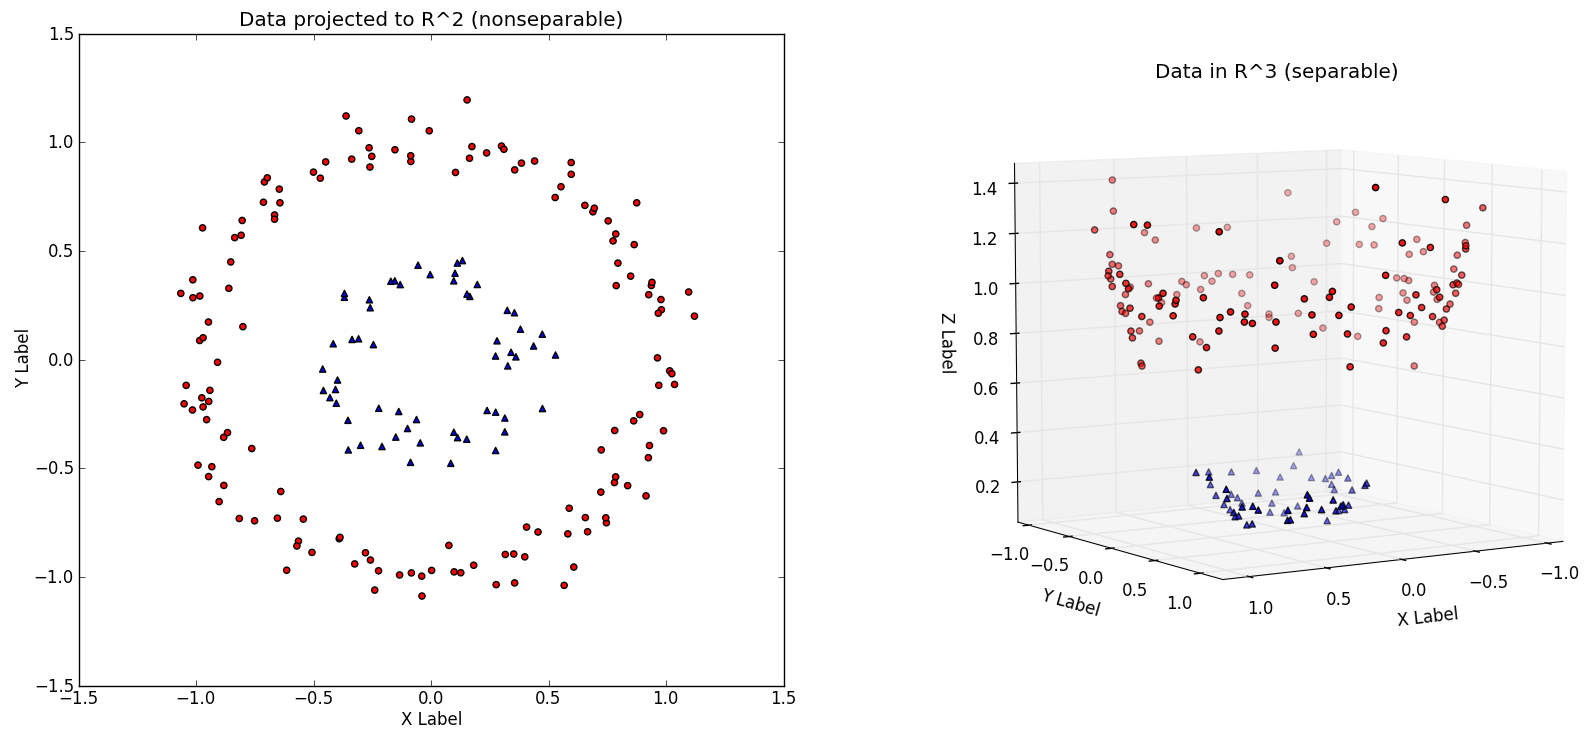
\includegraphics[width=0.5\textwidth]{fig/NonLinearDecisionBoudary2.png}
  	\caption{Données non séparable linéairement dans ${R}^{2}$ mais qui le devient dans ${R}^{3}$ avec $\phi({x}_{1},{x}_{2} ) = ({x}_{1},{x}_{2},{x}^{2}_{1}+{x}^{2}_{2})$ }
  	\label{fig:image16}
  \end{figure}\\
 \emph{\textbf{Définition  : Kernel}}
 Un Kernel est une fonction qui permet de calculer le produit scalaire du mapping d'un tuple dans un espace de dimension supérieur que celui dans lequel il est définie .
 on a : \\
 \begin{center}
 	${\large K }(x,z ) = {\phi}^{T}(x).{\phi}(z)$
 \end{center} 
 Mais on n'est pas obligé de connaitre ${\phi}(x)$ pour calculer ${\large K }(x,z ) $ il existe des Kernel bien définie qui permettent de calculer le produit scalaire sans pour autant connaitre $\phi$ et ainsi faciliter les calcul .\\
 En voici quelque uns les plus utilisé: \\
 - Le Kernel Polynomial de degré d : ${\large K }(x,z ) =({x}^{T}z+1)^{d}$\\
 - Le Kernel Gaussien :  ${\large K }(x,z ) = \exp( \frac{-{||x-z||}^{2}}{2{\sigma}^{2}})$ \\
 - Le Kernel sigmoïde :${\large K }(x,z ) = \tanh (k{x}^{T}y + \theta)$ \\
 
 Ainsi dans notre problème d'optimisation on peut juste remplacer le produit scalaire de ${x}_{i}$ et ${x}_{j}$ et ensuite palier aux problème des frontières de décisions non séparable linéairement.\\
 On choisie un Kernel en fonction des caractéristiques de l'ensemble d'apprentissage .\\
 Le problème sera    :
 \begin{center}
 	$ \left\{\begin{array}{ll}
 	max \sum _{i=1}^{m} {\alpha}{i} -  \frac{1}{2} \sum _{i=1}^{m} \sum _{i=j}^{m} {\alpha}_{i}{\alpha}_{j}{y}_{i}{y}_{j} {\phi}^{T}(x).{\phi}(y) ,&  \\
 	\mbox{Avec } \sum _{i=1}^{m}{\alpha}_{i}{y}_{i}=0 , & \\
 	\mbox{et }{\alpha}_{i} \ge 0 
 	\end{array}\right.$
 \end{center}
 Et en introduisant le Kernel on a :
  \begin{center}
  	$ \left\{\begin{array}{ll}
  	max \sum _{i=1}^{m} {\alpha}{i} -  \frac{1}{2} \sum _{i=1}^{m} \sum _{i=j}^{m} {\alpha}_{i}{\alpha}_{j}{y}_{i}{y}_{j} {{\large K }(x,y )},&  \\
  	\mbox{Avec } \sum _{i=1}^{m}{\alpha}_{i}{y}_{i}=0 , & \\
  	\mbox{et }{\alpha}_{i} \ge 0 
  	\end{array}\right.$
  \end{center}
  Et ainsi notre frontière de décision sera :
  ${\theta }^{T}{z} + b =  \sum _{i=1}^{m}{\alpha}_{i}{y}_{i}{{\large K }(x,y )} + b $ . \\
  Pour résoudre ce problème on utilise la méthode de ac{SMO} qui est la technique la plus utilisée pour la résolution de ces genres des problèmes , il est implémenté dans la plupart des package d'apprentissage automatique .
  \cleardoublepage
\subsection{Arbres des Decisons \cite{TreeBk1} \cite{TreeAV}}
\subsubsection{Définitions}
Une arbre de décision est un ensemble des règles de classification et de régression basant leurs décisions sur des tests associé aux attributs ,organisées de manière arborescente .\\
C'est une représentation d'une procédure d'apprentissage.\\
Voici quelques termes ou notions liées aux arbres de décisions:
\\
\emph{Noeud Principale ou Root Node} : c'est l'attribut qui se situe au premier niveau et sur base de celui- ci s'effectue notre prédiction.\\
\emph{Spliting ou segmentation}: c'est un processus consistant à diviser un nœud en 2 ou plusieurs sous nœuds sur base d'un test sur un attribue.\\
\emph{Nœud Interne ou Nœud de décision : } c'est un nœud étiqueté par un test qui peut être appliqué à toute description d'un individu de la population.\\
\emph{Une feuille :}
c'est le nœud où on ne peut plus diviser  ou segmenter l'arbre , il est étiqueté par une classe.
\subsubsection{Construction de l'arbre et Algorithme}
\paragraph{Mesure de la pureté des feuilles}
Pour Construire les nœuds de l'arbre,les  choix des « questions les plus discriminantes »  peuvent  se faire selon plusieurs critères : l’algorithme CART utilise l’indice de Gini, l’algorithme C4.5 utilise l’entropie, l'algorithme \ac{CHAID} utilise le test de khi carré, et plusieurs autres algorithmes.Dans cette partie nous ne parlerons que de deux premiers. Ces deux outils mathématiques visent à évaluer la « pureté » de chaque feuille : lorsque l’on se situe à un nœud donné de l’arbre, le but est de créer deux feuilles qui soient plus homogènes que le nœud qui
les précède. Il faut donc disposer d’un moyen de mesurer cette homogénéité, ou « pureté ». Grâce
à cela, à chaque nœud, le split est construit de manière à maximiser le gain d’information apporté
par une question donnée sur la connaissance de la variable réponse.
\subsubsection{Entropie}
L’entropie  est une fonction mathématique créée par Claude Shannon en 1948, pour des questions initialement liées à la théorie du signal.\\
En Machine Learning c'est la mesure du désordre ou de l'inégalité de répartition pour le choix d'un test à une position  de l'arbre.\\
Notons par E notre ensemble d'apprentissage divisé en classes ${\omega}_{1},{\omega}_{2},....,{\omega}_{k}$
- L'entropie de la distribution des classes = quantité moyenne d'information nécessaire pour identifier la classe d'un exemple de E.\\
 \begin{center}$ H(E)=-\sum _{j=1}^{k} P({\omega}_{k} ) \log_{2}({\omega}_{k})$\end{center}
 
où $ P({\omega}_{k} )$ est la probabilité a priori de la classe $ {\omega}_{k}$ \\
- Soit un test T(portant sur une variable X) ayant m alternatives possibles qui divisent En sous-ensembles $ {E}_{j}$ , caractérisé par une entropie $ H({E}_{j})$.\\
- L'entropie de la partition résultante, c'est-à-dire l'entropie conditionnelle de E étant donné T, est définie comme l'entropie moyenne des sous-ensembles:
\begin{center}$ H(E|T)=\sum _{j=1}^{j} P({E}_{j})H({E}_{j})$\end{center}
- Le gain d'information apporté par le test Test donc:
\begin{center}$ Gain(E,T)=H(E) - H(E|T)$\end{center}
L'algorithme de l'arbre de decisison se base sur ces propriétés.
\subsubsection{L'indice de Gini}
L’indice (ou coefficient) de Gini est une mesure, comprise entre 0 et 1, de la dispersion d’une distribution. Il est très souvent utilisé en économie ou en sociologie afin de mesurer les inégalités sociales au sein d’un pays. Dans ce contexte, plus le coefficient est proche de 1 et plus la société est inégalitaire.
il se calcule de la manière suivante :
\begin{center}
	$ Gini = \sum_{i\ne j} p({\omega}_{i})p({\omega}_{j})$
\end{center}
Avec $p({\omega}_{i})$ la probabilité de la classe $ {\omega}_{i} $ .\\
De la même façon que l'entropie on calcul le gain d'information avec l'indice de gini.
\subsubsection{Algorithme}
\begin{algorithm}
	\caption{Pseudo code de l'arbre de décision}
	\begin{algorithmic}
		\Require 
		Training set E \\
		\State Initialiser l’arbre courant `a l’arbre vide ; la racine est le nœud courant
	    \While{On n'as pas encore obtenu l'arbre}
	    \State Décider si le nœud courant est terminale
	    \If{le nœud est terminal } 
	    \State lui affecter une classe 
	    \Else 
	    \State Sélectionner un test et créer autant de nouveaux nœuds fils qu’il y a de réponses possibles au test
	    \EndIf
	    \State Passer au nœud suivant non exploré s’il en existe
	    \EndWhile
		\end{algorithmic}
		\end{algorithm}
\paragraph{}
En général, on décide qu’un nœud est terminal lorsque tous les exemples associés à ce nœud, ou du moins la plupart d’entre eux sont dans la même classe, ou encore, s’il n’y a plus d’attributs non utilisés dans la branche correspondante.
\paragraph{}
En général, on attribue au nœud la classe majoritaire (éventuellement calculée à l’aide d’une fonction de coût lorsque les erreurs de prédiction ne sont pas équivalentes). Lorsque plusieurs classes sont en concurrence, on peut choisir la classe la plus représentée dans l’ensemble de l’échantillon, ou en choisir une au hasard.
\subsubsection{Élagage de l'arbre ou \emph{Prunning}}
L'objectif de cette étape est de supprimer les parties de l'arbre qui ne semblent pas performantes pour
prédire la classe de nouveaux cas et les remplacées par un nœud terminal (associé à la classe majoritaire).\\
Le processus est remplacées par un nœud terminal (associé à la classe majoritaire).\\
il existe différentes façons d'estimer le taux d'erreur entre autre: \\
– sur base de nouveaux exemples disponibles;\\
– via une validation croisée ;\\
– sur base d'une estimation statistique, ex: borne supérieure d'un intervalle de confiance construit sur un modèle binomial .
\subsubsection{Avantages et inconvénients des arbres de décisions}
\paragraph{Avantages}
- Interprétabilité: chaque élément du modèle est facile à comprendre et à analyser pour un humain, et peut donner de l'information sur les données. Ceci est surtout vrai pour les petits arbres. À cause de l'instabilité des arbres (par exemple si on varie le choix des variables ou des données), il faut utiliser des techniques spécialisées pour determiner quelles variables sont réellement importantes. On peut faire correspondre un arbre de décision à un ensemble de règles SI-ALORS (en introduisant des nouvelles classes correspondant aux noeuds cachés de l'arbre).\\
- Flexibilité: peut être utilisé sur des données de n'importe quel type (dont évidemment les variables continues et discrètes) pour lesquelles un ensemble fini (pas trop grand) de questions possibles pour la partition peut être défini (en principe cela peut être appliqué à n'importe quel type de structures de données). \\
\paragraph{Inconvénients }

Un des inconvénients principaux des méthodes d'apprentissage par arbres de décision
est leur instabilité. Sur des données réelles, il s’en faut souvent de peu qu'un attribut soit
choisi plutôt qu'un autre et le choix d’un attribut-test, surtout s’il est près de la racine,
influence grandement le reste de la construction. La conséquence de cette instabilité
est que les algorithmes d'apprentissage par arbres de décision ont une variance importante, qui nuit à la qualité de l'apprentissage. Des méthodes comme le Bagging(pour Bootstrap Aggregating) ou les Random Forests(qui consiste à utiliser plusieurs arbres et utiliser le vote classe faite par chaque arbre pour classer une instance ) \cite{RandomForrest1} permettent dans une certaine mesure de remédier à ce problème.
\cleardoublepage
%\subsection{Segmentation  Par K-means }
La Segmentation est une technique d'apprentissage non supervisé, Les classes des données ne sont pas connus en avance .
La segmentation consiste à grouper les données dans des clusters ou segments selon leurs ressemblance , et leurs similarités. 
L'objectif de la segmentation est la maximisation des distances inter-cluster et la minimisation de la distance intra-cluster .
L'unité de mesure de la ressemblance entre les données c'est la distance . \\
Il existes plusieurs métriques pour définir la distance entre 2 points ${x}_{i}$ et ${y}_{i}$:  \\
- La distance euclidienne $d(x,y) = \sqrt{\sum_{i=1}^{n}({x}_{i}-{y}_{i})^2}$ \\
- La distance de Manhattan $d(x,y) = \sum_{i=1}^{n}|{x}_{i}-{y}_{i}|$ \\
- La distance de Minkowski $d(x,y) = \sqrt[q]{\sum_{i=1}^{n}|{x}_{i}-{y}_{i}|^p}$ \\
Supposons que nous disposons de m points $x_i$ que nous voulons segmenter en k clusters , l'objectif est d'assigner un cluster à chaque point .\\
 La methode K-means consiste à trouver les positions $\mu_k$  k = 1,2...K qui minimisent la distance distance du point aux cluster .
L'algorithme K-means consiste à résoudre le roblème suivant :\\
\begin{center}
	min $\sum_{i=1}^k\sum_{\b{x}\in c_i} d(\b{x},\mu_k)$
\end{center}
ou $c_i$  est l'ensemble des points appartenant au cluster i 
\subsubsection{Algorithme K-means }
\cleardoublepage
\section{Méthodologie de mise en place du processus de data mining\cite{DMProces}}.
Au début des années 90, l'intérêt croissant  pour le data mining a mis en lumière l'absence d'une méthodologie pour la mise en place d'un processus de découverte de connaissances, applicable quelle que soit l'industrie visée ou l'outil utilisé. De ce besoin est née l'initiative \ac{CRISP-DM}.
\begin{figure}[ht]
	\centering
	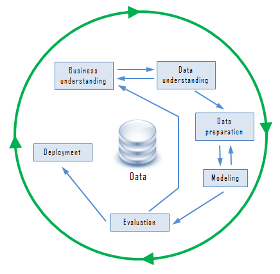
\includegraphics[width=0.5\textwidth]{fig/CRISP_tb.png}
	\caption[Short caption]{Data mining process model}
	\label{fig:imageCrisp}
\end{figure} 
A partir du processus de découverte de connaissances utilisé dans les premiers projets de data mining ,\ac{CRISP-DM} a défini et validé une méthodologie potentiellement applicable dans tous les secteurs de l'industrie. Elle permet de rendre les projets de data mining à grande échelle plus rapides, moins coûteux, plus fiables et surtout améliorer leur gestion. Cette méthodologie ne vise pas que les grands projets car même les petits projets de découverte de connaissances peuvent tirer profit de son utilisation.
Essentiellement, cette méthodologie fournit un aperçu du cycle de vie d'un projet de data mining. Elle identifie clairement les principales phases de ce processus au travers de tâches et des relations entre ces tâches. Même si le modèle ne le spécifie pas explicitement, il y a des relations possibles entre toutes les tâches en fonction des objectifs d'analyse et des données qui sont analysées.
Les six phases importantes du processus sont :
\begin{enumerate}
	\item \emph{La compréhension du problème métier} :  concerne la définition du problème d'analyse sur la base des objectifs métiers qui en sont à l'origine.
	\item \emph{La compréhension des données} :cette phase vise à déterminer précisément les données à analyser et à identifier la qualité des données .
	\item \emph{La préparation des données}: couvre les activités liées à la construction de l'ensemble précis des données à analyser à partir des données brutes. Ceci inclue le nettoyage des données, la sélection d'attributs, le choix des observations, etc.
	\item \emph{La modélisation }: est la phase consistant dans le paramétrage et le test de différentes techniques de data mining sur les données choisies, dans l'objectif d'optimisation du modèle ou des connaissances obtenues par ces techniques.
	\item \emph{L'évaluation }:vise à vérifier le modèle ou les connaissances obtenues afin de s'assurer qu'ils répondent aux objectifs formulés au début du processus. Elle contribue aussi à la décision de déploiement  du modèle ou, au contraire, de la nécessité que ce dernier soit reconstruit ou amélioré.
	\item \emph{Le déploiement }: est l'étape finale du processus de découverte de connaissances. Son objectif est de mettre la connaissance obtenue par la modélisation dans une forme adaptée et l'intégrer au processus de prise de décision. Le déploiement peut aller, selon les objectifs, de la simple génération d'un rapport décrivant les connaissances obtenue jusqu'à la mise en place d'une application spécifique permettant l'utilisation du modèle obtenu pour la prédiction des valeurs inconnues d'un paramètre d'intérêt.
\end{enumerate}

\cleardoublepage
\chapter{Analyse du domaine de l'orientation  \cite{OrBk1} \cite{OrBk2} \cite{OrBk3} \cite{OrBk4} \cite{OrBk5}}
\section{Généralités sur l’orientation des étudiants}
\paragraph{}
\ac {UNAF}  considère l’orientation comme un  véritable parcours, qui comporte des étapes  certes, mais qui doit s’inscrire dans la durée.  Cette inscription dans la durée nécessite que  des passerelles multiplient entre les différentes filières afin de permettre les  réorientations, même en cours d’année. Ces  passerelles devraient par ailleurs permettre  aux jeunes d’aller aussi loin qu’ils le désirent  dans leurs études, quel que soit leur choix  initial. Ainsi l’orientation pourra être  dédramatisée et aucune formation choisie ne  sera une « voie sans issue ».  Ce serait aussi un moyen de lutter contre la  déscolarisation qui provient souvent d’un  choix d’orientation qui ne convient pas et qui  pousse les jeunes à arrêter complètement leur  scolarité au lieu de se réoriente
\paragraph{}
En effet, le terme “orientation” recouvre deux activités que la langue anglaise distingue : le processus qui répartit les élèves dans différentes voies de formation, filières et options (“students distribution”) ; l’aide aux individus dans le choix de leur avenir scolaire et professionnel (“vocational guidance”, “school and career counseling”).
\paragraph{}
Face à la crise, le diplôme protège du  chômage et favorise l’accès à la  formation continue.  Le rapport  « Formations et emplois » de l’Insee (2013), fait preuve qu’environ 800 000 élèves sont inscrits en  troisième et 700 000 sont candidats au  bac. Il s’avère important de savoir si chacun trouvera-t-il la place qui  lui convient pour la suite ? Ce n’est pas si facile, car la plupart des filières imposent une sélection à  l’entrée, en fonction du nombre de  places disponibles
\paragraph{}
La difficulté face à un choix d’orientation,  légitime à l’adolescence, peut être  handicapante par la suite, d’où la nécessité  d’une réelle  éducation au choix, à l’orientation qui prennent en compte les trois  volets : connaissance de soi, connaissance  des métiers et de l’environnement  professionnel, connaissance des formations. Cependant, au final, faute d’avoir trouvé sa voie ou acquis le niveau nécessaire, un nombre important d’élèves quitte chaque année le système éducatif sans avoir obtenu de qualification. 
\paragraph{}
A ce propos, le rapport  haut conseil d’éducation(2008) stipule que chaque année 120 000 jeunes quittent le  système de formation initiale sans  diplôme (surtout dans la voie  professionnelle). A l’université, le  décrochage concerne 80 000 jeunes par  an (1/4 de l’ensemble des sortants de  l’université d’une année). Les services qui s’occupent de  l’orientation sont éparpillés, il existe un accès inégal à ces services,  les ressources humaines et matérielles limitées influent sur la qualité des services offerts Pourtant, l’objectif des universités vise à offrir une bonne démarche d’orientation aux  étudiants. Elles ont comme défi d’élaborer  pour chaque étudiant une démarche d’orientation stimulante, cohérente, réaliste et adaptée à sa dynamique personnelle, d’établir une véritable culture d’orientation en impliquant, d’une part, tout le personnel de l’université, les amis et la famille de l’élève ainsi que les partenaires de la communauté et, d’autre part, en unissant les forces du réseau d’intervenants qui soutiennent les étudiants sur le plan personnel et professionnel pour faciliter leur insertion dans notre société
\paragraph{}
L’orientation au collège et au lycée est  déterminée par les notes qui répartissent  les élèves de manière hiérarchisée, et non  sur les appétences et potentialités  personnelles. (Au collège plus de 4 élèves  sur 10 estiment donc que leur orientation  est subie plus que choisie), elle peine à encourager les  jeunes issus des milieux les moins  favorisés, elle est trop irréversible c'est-à-dire absence de passerelles et de réorientation  entre voie professionnelle et voie  technologique et générale mais aussi elle est conditionnée par l’offre  de formation de proximité et cette offre  de formation est mal répartie sur le  territoire. On constate également la mobilité des élèves qui est faible, d’où  l’offre de formation ne s’adapte que  lentement aux nécessités économiques ce qui conduisent  les jeunes à s’engager  parfois dans des filières sans perspective. 
\paragraph{}
Ainsi, actuellement en \ac{RDC}, aucune structure d’orientation scolaire et professionnelle n’existe et le pouvoir public n’y pense même pas. Avec la prolifération des Instituts Supérieurs et des Universités publics ou privés, créées anarchiquement par le pouvoir public depuis des décennies, les élèves finalistes de l’enseignement secondaire s’orientent en considérant, en fin de compte, l’implantation géographique de ces établissements. Le système de prime qui a été instauré depuis les années 1992 complique encore davantage le système d’orientation des élèves. Les enfants issus des catégories sociales défavorisées embrassent, pour la plupart, les études dans les institutions publiques qui coûtent moins cher comparativement aux institutions privées. De ce fait, beaucoup d’élèves effectuent le choix des études aléatoirement sans tenir compte des aptitudes intellectuelles ou des aspirations professionnelles futures. Les jeunes sont donc abandonnés à leur triste sort. Cette situation étant considérée comme étant normale, personne n’en fait nullement allusion.
\section{Présentation du service de l’orientation des étudiants}
\textbf{\textit{Qui intervient dans le processus d’orientation ?}} \\

L’élève en quête d’orientation n’est pas laissé à lui-même.  Outre sa famille, il peut requérir l’aide de ses parents, de ses enseignants, du directeur d’établissement et des conseillers.
\begin{enumerate}
	\item \textit{\textbf{les parents: }} \\
	Parmi les acteurs de l’orientation, les parents sont bien entendu les premiers concernés. Si le rôle des parents est irremplaçable, c’est  avant tout parce qu’ils sont probablement seuls capable d’aimer l’enfant de manière inconditionnelle, indépendamment de ses résultats scolaires et autres performances. Ils sont les seuls à continuer à croire en l’enfant, lorsque les autres désespèrent. Et l’une des fonctions parentales est justement de construire l’estime de soi de leur enfant.
Ils interviennent pour trois objectifs qui sont :	
-  améliorer l’orientation afin qu’elle soit choisie plutôt que subie
-  renforcer les relations école-famille 
-  prévenir le décrochage scolaire
Les jeunes confrontés aux choix d’orientation ont besoin  d’une écoute attentive de la part de leurs parents. Les parents  ne sont pas forcément aux faits des filières de formation et  ne connaissent pas tous les métiers mais ils peuvent être au  jour le jour un soutien pour leur enfant qui s’interroge.
		\item \textit{\textbf{Les enseignants}} \\
		Dont l’action même d’enseigner est partie prenante de l’orientation et qui doivent aussi y exercer une mission précise.
Quoiqu’il en soit, en matière d’orientation, les enseignants exercent une influence déterminante par la seule mise œuvre de leurs démarches pédagogiques. Ils disposent, par les outils et les méthodes qu’ils utilisent ainsi que par leur comportement, des moyens d’agir sur certains éléments constitutifs de la maturation des choix de l’élève, particulièrement sur l’image qu’il se forge de lui. Les enseignants aident l’élève à prendre conscience  de ses potentialités et guide ses choix d’orientation.  
	\item \textit{\textbf{Le chef d’établissement}} \\
	Le chef d’établissement joue aussi un rôle fondamental dans la préparation de ses élèves à l’orientation. Il est responsable du dispositif d’orientation mis en place dans son établissement. C’est sous sa responsabilité que le programme d’information et d’orientation s’élabore et s’applique. Il est le garant du respect des réglementations en vigueur, mais au-delà il imprime selon ses convictions son expérience et les caractéristiques des populations dont il a la charge, le mouvement qui induit généralement à une véritable politique de l’information et de l’orientation. Il a un rôle particulièrement important dans la mise en œuvre des procédures d’orientations, dans le déroulement du dialogue avec les parents et dans le suivi des décisions.
	\item \textit{\textbf{Le conseiller d'orientation}} \\
	Les tâches du conseiller d’orientation dans une école s’avèrent multiples et difficiles à accomplir par lui seul car c’est un travail qui requiert la collaboration de différents acteurs comme nous l’avons signalé ci-dessus. L’une de ses missions consiste à fournit les informations.
	Le processus de cette action d’information est de :
	-	Mettre l’élève en état de réceptivité ;
	-	Proposer des informations en rapport avec les intérêts connus ;
	-	Adapter le message au niveau de l’élève et pour cela, il faut donner des propositions supplémentaires et faire des synthèses nécessaires avec la participation de l’élève.
	Le but à atteindre est de mettre l’élève en état de réaliser une self-orientation. De plus, le conseiller a le devoir de fournir aux parents des informations nécessaires pour qu’ils puissent assurer leurs responsabilités vis-à-vis de leurs enfants.
\end{enumerate}
\section{Etude des procédures d’orientation }
L’orientation et les formations proposées  aux élèves tiennent compte de leurs  aspirations, de leurs aptitudes et des  perspectives professionnelles liées aux besoins  prévisibles de la société, de l’économie et de  l’aménagement du territoire. \\
Dans ce cadre,  les élèves ou les étudiants élaborent leur projet d’orientation  scolaire et professionnelle avec l’aide des  parents, des enseignants, des personnels  d’orientation et des autres professionnels compétents, etc. Le chef d’établissement, décideur final, en l’état actuel du système, c’est lui qui prend la décision finale d’orientation, sur  proposition des membres du conseil de classe.
\begin{itemize}[label=\textbullet]
	\litem{Un conseil personnalisé : } \\
	Cette méthode s’appuie sur l’échange et le dialogue et permet de déceler des potentiels sans intervenir de manière directive dans les réponses et les choix du candidat.
 
           A l’aide de tests validés par des psychologues d’une part, et d’entretiens non directifs d’autre part, le conseiller définit des profils de métiers et d’études en adéquation avec les motivations, les aptitudes et la capacité de travail. Il tient compte des débouchés réels offerts par le marché du travail. Cette méthode permet de s’adapter et de respecter la personnalité de chacun en construisant ensemble un projet d’orientation.
	\litem{Le bilan d’orientation : } \\
	
	Destiné à tous les élèves à partir de la 3ème, ainsi qu'aux étudiants en recherche de réorientation, ce bilan permet de prendre les bonnes décisions d’orientation, en toute connaissance de cause. Le bilan d'orientation se déroule en 3 phases :
Phase 1 : Exploration
Ce premier rendez-vous permet de recueillir vos motivations et vos aspirations et d'évaluer vos aptitudes, etc. Cette phase s’appuie sur : des entretiens non directifs
 l'évaluation des aptitudes de l’étudiant ;  et un test concernant ses motivations, sa personnalité, ses  centres d'intérêt ...  \\
Phase 2 : Analyse et Synthèse
Le conseiller effectue une synthèse des résultats obtenus à l’aide d'un logiciel développé au Canada et utilisé depuis plus de 30 ans, etc. Ce logiciel a reçu le label \ac{RIP}  du ministère de l'Education Nationale, il est remis à jour chaque année. Il bâtit ensuite un projet d’orientation cohérent. \\
Phase 3 : Restitution des résultats
Lors du  deuxième rendez-vous, le conseiller propose à l’étudiant une sélection de métiers et de formations. Un rapport écrit contenant des fiches métiers (descriptif, niveau de formation à atteindre, perspectives d'emploi ...) et des informations sur les formations à suivre vous est remis.

\end{itemize}

\section{Etudes des documents utilisées}
\begin{itemize}[label=\textbullet]
	\item Dossiers scolaires et psychologiques \\
	Les données de toute étude pédagogique et psychologique en orientation  sont contenues dans le dossier scolaire et le dossier psychologique établis pour chaque élève à un moment de sa scolarité, puis complétés au cours de ses études à l’aide des informations scolaires, familiales, psychologiques, qui permettront au conseiller psychologue de suivre son évolution et de donner un conseil d’orientation au moment du choix scolaire ou professionnel.
Son but est de : 
	\begin{itemize}
		\item Connaitre l’élève au cours de son évolution ;
		\item Etudier les facteurs de réussite ou d’échec qui sont apparus au cours de cette évolution ;
		\item En rechercher les causes et trouver les remèdes s’il le faut
	Son contenu est  constitué par les données quantitatives et qualitatives.
		\begin{enumerate}
			\item Les données quantitatives : sont des résultats obtenus:\\
				\begin{itemize}
					\item D’une part aux examens écrits ou oraux.
					\item D’autre part aux tests d’aptitudes et de connaissances.
				\end{itemize}
			\item Les données qualitatives : \\
			 sont recueillies par les tests de personnalité et les entretiens. Elles sont complétées par les comptes rendus des conseils de classe, de délibérations….
		\end{enumerate}
	\end{itemize}
	\item Analyse du dossier psychologique\\
	Afin d’obtenir la vue la plus objective possible de l’enfant, les différents éléments des dossiers sont analysés de façon à permettre des confrontations et de recoupements
\begin{enumerate}
	\item les données physiologiques : \\
	vision, audition, motricité, fatigabilité, déficience, etc. sont obtenues grâce à l’étude :\\
	\begin{itemize}
		\item De la fiche médicale,
		\item Des questionnaires (élèves-parents-enseignants),
		\item Des examens psychologiques.
	\end{itemize}
	\item les données mentales :\\
	 efficience, mémoire (formes), intelligence (niveau, attitudes, facteurs spécifiques..,), aptitudes particulières (scientifiques, littéraires, artistiques…) sont apportées par :
	 	\begin{itemize}
	 	\item La fiche scolaire,
        \item Les questionnaires (élèves-parents),
		\item L’examen psychologique.
		\end{itemize}
	\item les données scolaires (niveau d’acquisition scolaire…) sont fournies par :\\
			\begin{itemize}
			\item La fiche scolaire ou bulletin,
			\item Les tests de connaissances scolaires.
			\end{itemize}
	\item le données caractérielles :\\
	activité ou passivité, sens de l’effort, émotivité, affectivité, attitude devant le travail, attitude à la maison, à l’école, attitude devant la réussite, devant l’échec, attitude envers les parents, enseignants, élèves…sont apportées par :
	\begin{itemize}
	\item	Les questionnaires,
	\item	Les entretiens,
   	\item    Les épreuves psychologiques particulières (les tests projectifs).
	\end{itemize}
\end{enumerate}
\end{itemize}
\paragraph{}
Notons également que quand le dialogue entre l'équipe éducative et la famille n’a pas permis d'aboutir à une  décision commune, les parents peuvent engager une procédure d'appel regroupant la commission d’appel. Cette dernière est présidée par  le directeur des services académiques, ayant l’objectif de réexaminer la décision d'orientation  en fonction des notes de l'élève, de ses capacités, de ses difficultés, de ses projets. Son point  de vue est extérieur.  Ainsi, les membres de la commission (chefs d'établissement, professeurs,  conseillers d’orientation...) ne sont pas directement impliqués dans l’histoire scolaire de  l’élève.
\section{L'orientation à l' \ac{ULPGL} /GOMA  \cite{OrBk6} }
Abordant la question de l’orientation à \ac{ULPGL} est assurée par l’apparitorat  central et la direction de scolarité. 
\paragraph{}
Dès son arrivé à l’université, on présente au candidat un papier sur lequel toutes les facultés sont mentionnées ainsi que les orientations, mais en plus les exigences pour chaque faculté. 
 A part cela, l’étudiant doit écrire une lettre manuscrite, et doit compléter une fiche de demande d’inscription, et déposer son dossier contenant : son diplôme d’Etat ou son équivalent, une attestation de naissance, une attestation de bonne vie et mœurs, une attestation de célibat, une attestation de nationalité, une attestation de résidence  (pour les étrangers) et un certificat d’aptitude physique. Après avoir fournis tous ces éléments, la direction de scolarité va siéger et analyser le dossier du candidat avant de le soumettre à un examen écrit.   
Un examen est organisé pour les étudiants ayant obtenu moins de soixante pourcent. Ce concours est organisé en deux moments. Le premier concours se déroule au mois de septembre et le deuxième concours avant la rentrée académique  pour permettre à ceux qui ont raté le premier examen de se rattraper et être éligible. Les résultats obtenus à ce concours sont affichés à la valve et la commission chargé des inscriptions, dirigé par le secrétaire général académique décide si le récipiendaire est retenu, rejette ou réorienté dans une autre faculté compte tenu de ses résultats obtenus. 
\paragraph{}
Concernant l’orientation proprement dite, la direction de scolarité explique aux étudiants comment fonctionne chaque faculté de l’université, les exigences, les débouchés sur le milieu professionnel et chaque étudiant choisi sa faculté compte tenu de ses choix, ses gouts, ses aspirations, ses motivations, ses objectifs et sa vision sans pour autant le contraindre. Cependant la contrainte intervient au cas où, l’étudiant a choisi une faculté qui ne correspond pas à sa capacité intellectuelle, mais en plus si l’étudiant échoue ou produit un résultat moins satisfaisant à la fin d’une année académique, la direction de scolarité décide de le mettre en  observation, après les examens du premier semestre ils peuvent décider de le réorienter dans une autre faculté où il peut s’en sortir mieux.  Si cette orientation ne produit pas des résultats satisfaisants la commission décide du refus, ou du renvoi de l’étudiant de l’université car il est  \ac{INAPS} ou il a épuisé toutes les possibilités qui lui ont étés offertes. 

\cleardoublepage
\chapter{Présentation et Exploitation des Données Obtenues}
\paragraph{}
 Dans ce chapitre nous allons exploités les données mise en notre
disposition par les autorités de l'\ac{ULPGL}. Celles-ci sont issues du
système d'information \ac{UAT}  et pour des
raisons de confidentialité nous n'avons pas eu accès a toute la base des
données nous avons juste fais une requête des donnes dont nous avons
besoin pour notre étude et l'administrateur a exécuté une requete vers
sa base des données et nous a fourni les données dont nous avions besoin
pour l'étude sous forme d'un fichier \ac {CSV}. Comme
souligné dans le chapitre premier ce chapitre se basera sur la
méthodologie \ac{CRISP-DM} elle sera subdivisé en différentes sections:
\begin{itemize}
	\item L'exploration et la préparation des données 
	\item  Construction du modèle de Prédiction  
	\item  L'amélioration du modèle  \cite{bookSckit-Learn}
\end{itemize}


    \section{Exploration et la préparation des donnés}
\paragraph{}
Les spécialités affirment que 70-80 \% du temps consacré à un projet
DataMining est alloué à la phase de l'exploration et la préparation des
données \cite{DataExpAV} , il n' ya pas des raccourcis pour cette phase et si on l'a pas
bien effectué nous risquons de nous retrouver entrain d'améliorer
l'exactitude de notre algorithme mais en vain nous serons toujours
obligées de retourner à cette phase et toutes ces techniques de
l'exploration des données pourrons nous venir en aide .\\
Les Étapes de la phase d'exploration et la préparation des donnes sont mentionnées sur la figure suivante :
\paragraph{}
En bref l'exploration des données consiste à se plonger dans le passée
pour prédire l'avenir .Souvenons nous que la qualité de notre entré
détermine la qualité de notre sortie, ces phases nous permettent
d'améliorer la qualité de notre entré en vue d'avoir une bonne sortie.
Voici les étapes de cette phases:
\begin{figure}[ht]
	\centering
	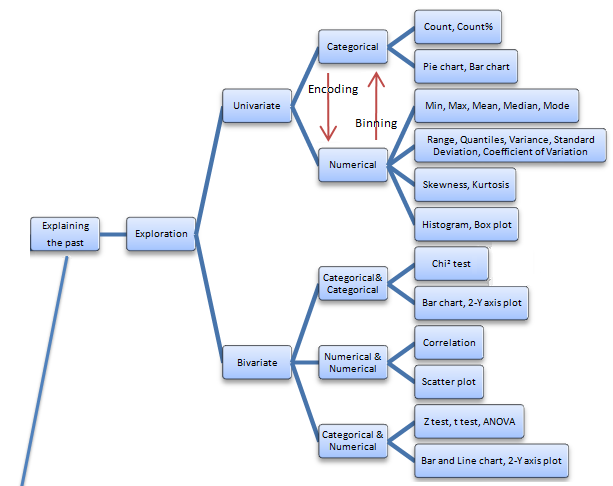
\includegraphics[width=0.5\textwidth]{fig/Exploration.png}
	\caption[Short caption]{Étapes de la phase d'exploration des données }
	\label{fig:imageExpSt}
\end{figure} 
\begin{itemize}
\item
  Identification des variables
\item
  Statistique Descriptive
\item
  Analyse Bi-varié
\item
  Traitement des valeur manquantes
\item
  Traitement des déviations  ou valeurs aberrantes (\emph{Outliers})  
\item
  Transformation des variables
\item
  Création des nouvelles variables
\end{itemize}
Comme nous l'avons soulignées dans le chapitre 1 ce processus est un
processus itératif et incrémentai nous exécuterons cette phase 2 a 5 fois ou plus en vue d'avoir un bon modèle.
\subsection{Identification des Données et des Variables}
\paragraph{}
Comme soulignées dans la phase d'introduction les données mise à notre
disposition sont sous format \ac {CSV} et nous allons utilisé la librairie pandas de python pour faire l'analyse , nous utiliserons aussi d'autres libraires qui nous permettrons de faire les statistiques ainsi que les visualisations :
Nous remarquons que les données sont stocké dans un e structure de type
matricielle appelé Dataframe. \cite{pedregosa2011scikit}
Un DataFrame selon la documentation officielle de pandas est une
structure des données bidimensionnel avec des colonnes des données des différentes types . Il peut être comparée à une feuille de calcul Excel ou une table dans \ac{SQL}.
Notre ensemble d'apprentissage de départ est une matrice de 9606 lignes et  22 colonnes .\\
Chaque ligne comprend les informations d'un étudiant pour une année académique et voici la description des nos colonnes.\\ 
\begin{multicols}{2}
	\begin{enumerate}
	 \item IDENTIFICATION : contient une identification unique et anonyme d'un étudiant les noms et les matricules réels des étudiants on éé cachées
	pour des raisons de confidentialités
	
	\item BIRTHDAY : contient la date de naissance de chaque étudiant
	
	\item NAME : contient le sexe de chaque étudiant
	

	
	\item DIPLOMTYPE : le type de diplôme
	
	\item DIPLOMMENTION : mention de diplôme
	
	\item  DIPLOMPERCENTAGE: le pourcentage au diplôme
	
	\item DIPLOMSECTION: la section du diplôme
	
	\item DIPLOMOPTION : l'option
	
	\item  DIPLOMPLACE : l'endroit d'obtention du diplôme
	
	\item SCHOOL : l'école de provenance
	
	\item  SCHOOLPROVINCE : la province de provenance
	
	\item  SCHOOLCODE : code de l'école
	
	\item SCHOOLSTATUS : le statuts de l'école (privée , publique ,
	conventionné ,..)
	
	\item  ACADYEAR : l'année académique
	
	\item  PERC1 : pourcentage en première session
	
	\item  MENT1 : mention en première session
	
	\item  PERC2 : pourcentage en seconde session
	
	\item  MENT2 : mention en seconde session
	
	\item  FAC : la faculté de l'étudiant 
	
	\item  OPT : l'option choisie par l'étudiant
	
	\item  PROM : la promotion de l'étudiant 
	\end{enumerate}
\end{multicols}

 Comme nous pouvons le constater les colonnes 1-13 regorgent les informations que chaque étudiant donné à son inscription , ils constituerons nos variables d'entres les restes seront utilisées pour constituer notre variable de sortie.

Nous l'avons aussi signales que chaque ligne comprend les information
d'un étudiant pour une année académique . Pour mener bien notre analyse nous allons grouper les information de chaque étudiant en une ligne nos données seront groupé selon les variables d'entrées ensuite les donnés de sorties seront groupes selon une fonction d'agrégation prédéfinie.
Nous allons premièrement faire une analyse uni-varié  sur les données en entrées !
Soulignons que nous avons décidé de supprimer certaines colonnes n'ayant pas des informations importantes car contenant plus de 90 \% des valeurs manquantes il s'agit entre autres des colonnes suivantes :
'DIPLOMDATE','DIPLOMMENTION','DIPLOMPLACE','SCHOOLCODE'.

Après suppression les colonnes en entrée deviennent les 10 premiers colonnes.

Pour une première approche nous allons grouper notre ensemble en fonction des données en entré et ensuite écrire une fonction qui va grouper les donnes de sortie la fonction de qui regroupe les données en sortie ne fait que grouper les mention , et pourcentage pour une année académique d'un étudiant dans une liste.\\ 
Après groupement en fonction des matricules nous venons de remarquer que
notre ensemble comprend 4715 lignes et 18 colonnes et c'est sera notre ensemble pour notre étude ,cet ensemble est subdivisé en variables d'entré et variables de
sortie!\\
Voici un aperçu des nos données en entrée ainsi que les données en sorties  au tableau la figure la figure \ref{tab:Dataset}
\paragraph{}
Nous venons de finir avec la présentation des nos données nous allons
maintenant débuter avec la phase d'analyse promptement dite  des donnés que nous avons en entré et ensuite nous effectuerons  une analyse des données en
sortie en enfin analyse les donnes des sortie combinées à celles des données  en entrée
\begin{sidewaystable}
	\centering
	\begingroup % make the next setting local
	\captionsetup{type=table} % here we want to caption a table
	\caption{Bref aperçu de notre ensemble d'apprentissage }
	\label{tab:Dataset}
	\begin{tabular}{lllllr}
		\toprule
		{} & SCHOOLSTATUS &   SCHOOL\_RIGHT &         OPTION\_RIGHT & SCHOOLPROVINCE &  DIPLOMPERCENTAGE \\
		\midrule
		45  &   protestant &         zanner &  commmerciale et adm &      NORD-KIVU &         61,000000 \\
		215 &     publique &       chemchem &            pedagogie &        MANIEMA &         51,000000 \\
		343 &   catholique &        kambali &           bio-chimie &      NORD-KIVU &         62,000000 \\
		356 &   catholique &  mwanga/ uvira &          latin philo &       SUD-KIVU &         51,000000 \\
		429 &   protestant &      maendeleo &              inconnu &      NORD-KIVU &         56,876522 \\
		474 &   protestant &      maendeleo &          latin philo &      NORD-KIVU &         56,000000 \\
		644 &     publique &          ngoma &        math-physique &      NORD-KIVU &         68,000000 \\
		645 &     publique &          ngoma &            pedagogie &      NORD-KIVU &         59,000000 \\
		\bottomrule
	\end{tabular}
	\begin{tabular}{lrlllllll}
	\toprule
	{} &   ID &                ACADYEAR &                  PERC1 &     MENT1 &                 PERC2 &       MENT2 &   FAC &      PROM \\
	\midrule
	0 &   45 &             [2013-2014] &                  [nan] &      [AA] &                 [nan] &       [nan] &  FPSE &      [L2] \\
	1 &  215 &             [2012-2013] &                  [nan] &     [ADM] &       [63.0999984741] &         [S] &    FD &      [L2] \\
	2 &  343 &             [2015-2016] &                  [nan] &      [AA] &       [52.2000007629] &         [A] &  FSEG &      [G2] \\
	3 &  356 &             [2015-2016] &                  [nan] &   [ADSTM] &       [59.9000015259] &         [S] &  FSEG &      [L2] \\
	4 &  429 &             [2013-2014] &                  [nan] &      [AA] &                 [nan] &         [A] &    FD &      [G1] \\
	5 &  474 &  [2014-2015, 2015-2016] &            [nan, 62.5] &   [AA, S] &            [nan, nan] &  [nan, nan] &    FD &  [G3, G3] \\
	6 &  644 &  [2013-2014, 2014-2015] &  [60.4000015259, 68.0] &    [S, S] &            [nan, nan] &  [nan, nan] &    FD &  [L1, L2] \\
	7 &  645 &  [2014-2015, 2015-2016] &             [nan, nan] &  [AA, AA] &  [61.4000015259, nan] &    [S, NAF] &    FD &  [L1, L2] \\
	\bottomrule
\end{tabular}
\endgroup
\end{sidewaystable}
 \subsection{Préparation des données }
Cette phase consistera aux traitement des valeurs manquantes et valeurs aberrantes mais aussi au nettoyage des données mal orthographiées lors de la saisie des données pour certaines attribues. 
Commençons par  Expliquer les raisons de la présence des valeur manquantes , ainsi que les données aberrantes et la manière de les traiter
\paragraph{}
Malgré la quantité croissante de données, les problématiques de données
manquantes et des valeurs extrêmes restent très répandues dans les
problèmes statistiques et nécessitent une approche particulière. Ignorer
les données manquantes et les valeurs extrêmes peut entraîner, outre une
perte de précision, de forts biais dans les modèles d'analyse et comme
signaler dans l'introduction de ce chapitre peuvent augmenter l'erreur
de prédiction.
\subsubsection{Valeurs Manquantes}
\paragraph{Cause et types des Données Manquantes} \cite{MissinVal}
Les \ac{DM} ont de multiples causes. Il peut être
impossible de contacter une personne sélectionnée pour faire partie
d'une enquête (non-réponse totale) ou un répondant peut refuser de
répondre à une ou plusieurs questions (non-réponse partielle). Une
mauvaise saisie de l'information peut également générer des \ac{DM}.
Finalement,des \ac{DM} peuvent aussi être causées par l'existence de données
aberrantes qui doivent être supprimées avant d'effectuer des analyses.
Selon les cause on classe les données manquantes selon différentes types
il existe plusieurs types de données manquantes, ils peuvent être introduit lors de :
\begin{enumerate}
\item  l'extraction des données :
il peut être possible qu'on ait des problèmes lors de l'extraction des données 
dans ce cas il es préférable de vérifier les données avec les donateurs c'est comme par exemple pour notre étude dans une première approche nous n'avons pas réussie les données des étudiants ayant passer en première session 
certaines fonctions peuvent aussi créer des données manquantes comme c'est le cas de notre fonction qui calcule les dates '
ces genres des données peuvent facilement être détecter.
\item  la collecte des données ;
c'est le cas le plus courant et il est plus facile de le détecter.
\end{enumerate}

Dans ce cas la classification la plus couramment utilisée ayant été
proposée par Little et Rubin \cite{MissinVal} : 
\begin{itemize}
	\item  Missing completely at random (MCAR) (complètement aléatoire)
	\item Missing at random'' (MAR) (aléatoire)
	\item Missing not at random'' (MNAR) (non aléatoire)
\end{itemize}
\subparagraph{}
 Les DM sont MCAR lorsque la probabilité de non réponse pour une variable ne
dépend pas de celle-ci, mais uniquement de paramètres extérieurs,
indépendants de cette variable. Cela veut dire qu'il n'est pas possible
de défi- nir un profil des individus ayant des DM et que la probabilité
des DM est uniforme. De manière générale, ce type de DM est très rare.
\subparagraph{}
Les DM sont dites MAR lorsque la probabilité de non-réponse peut
dépendre des observations mais pas des DM, par exemple s'il existe une
différence de non-réponse entre les hommes et les femmes concernant la
question du revenu, mais que parmi les hommes entre eux ou parmi les
femmes entre-elles, la probabilité d'avoir des non-réponses est
identique quel que soit le niveau du revenu.
\subparagraph{}
Finalement, les DM sont de type MNAR lorsque la probabilité de
non-réponse est liée aux valeurs prises par la variable ayant des
DM.comme par exemple pour notre cas les étudiant n'ayant pas passé tous
leurs examens à une session n'ont pas des pourcentage à cette session et
on pour mention AA assimiléé aux ajournées .

\paragraph{Méthodes d'imputations} 

Il existe 8 à 9 méthodes de traitement des données manquantes
largement répandues à l'heure actuelle, y compris des méthodes connues
pour être peu performantes mais cependant toujours utilisées. 
\begin{enumerate}
	\item Analyse des cas complets (CC)
	\item Imputation par la moyenne (MEAN) : c'est la
	méthode que nous utiliserons par défaut
	\item Imputation par la médiane
	(MED)
	\item  Imputation par régression simple (REG)
	\item Imputation multiple par Markov Chain Monte-Carlo (MCMC)
	\item  Imputation par le plus proche
	voisin (KNN)
	\item Imputation multiple par un algorithme basé sur le
	bootstrap, approchant des résultats de l'algorithme EM (EM)
	\item Imputation multiple par ``Predictive Mean Matching'' (PMM)
\end{enumerate}
Toutes ces techniques existe sont implémentées dans les librairies que nous
utilisons.\\
Dans ce travail selon le cas nous allons faire une imputation par la
moyenne ou par analyse des cas complets mais soulignons qu'il faut bien
réfléchir avant d'utiliser une imputation par la moyenne car il a une
mauvaise influence sur la variance
\subsubsection{Valeurs aberrantes ou extrêmes ou outliers}
Une valeur aberrante est une valeur qui diffère de façon significative
de la tendance globale des autres observations quand on observe un
ensemble de données ayant des caractéristiques communes. Par exemple
dans l'analyse des pourcentage du diplôme à l'EXETAT nous avons trouvé
des diplôme qui ne sont pas dans l'intervalle 0 à 50 \% des étudiant
avec des diplômes de 634\% ou des diplômes de 0\%

Voici quelque remarques à considérer pour les valeurs aberrantes :
\begin{enumerate}
	\item Les valeurs aberrantes ne sont pas forcément erronées. Dans certains
	cas, la valeur aberrante doit être acceptée comme une indication
	intéressante. par exemple après analyse on trouve une étudiant âge de 60
	ans! 
	\item Il ne faut pas adopter une attitude radicale de rejet, ou
	d'inclusion systématique des valeurs aberrantes. Le rejet systématique
	peut entraîner la perte d'informations réelles Le rejet des valeurs
	aberrantes a des conséquences statistiques non négligeables car
	l'analyse est ensuite faite sur un échantillon censuré qui n'est plus
	aléatoire.
\end{enumerate}
En fonction des circonstances, il existe des méthodes,
dites robustes, qui prennent en compte toutes les données mais
minimisent l'influence des valeurs aberrantes. 
L'apparition de valeurs aberrantes est due à diverses sources de natures différentes, d'où la
complexité de l'examen des valeurs aberrantes.

Pour détecter les valeurs manquantes nous avons utiliser les techniques
suivantes :

\begin{enumerate}
	\def\labelenumi{\alph{enumi})}
	\item
	Contrôle sur le domaine des valeurs : Exemple : Pour la variable «
	DIPLOMPERCENTAGE », une borne maximale (100 \% ) est connue et la
	valeur minimale est de 50 . Les valeurs supérieures à 100 et
	inférieur à 50 sont considérés comme aberrantes.
	\item
	Détection graphique : Pour détecter la présence de valeurs aberrantes
	On a utilisé :
\end{enumerate}

\begin{itemize}
	\item
	Boxplot
	\item
	diagramme de dispersion des observations classées en fonction de leur
	rang
\end{itemize}

\paragraph{Traitement des valeurs aberrantes :}
\begin{enumerate}
	\item  Les valeurs aberrantes pouvant provenir d'erreurs de saisie, on le traite séparément
	en étudiant cas par cas.c'est cette technique que nous allons utilisé
	pour certaines valeur du pourcentage de diplôme.
	\item On les rejette et on applique ensuite une des méthodes d’imputation (moyenne,médiane…) vues pour les valeurs manquantes.
	\item  On adopte des méthodes qui diminuent leur impact au cours des analyses statistiques :la médiane
\end{enumerate}
Voici Un aperçu des nos colonnes avec données manquantes et données aberrantes
ce tableau décrit.
\begin{table}
\centering
\begingroup % make the next setting local
\captionsetup{type=table} % here we want to caption a table
\caption{Statistiques Des Données avec Valeurs manquantes et abberantes}
\label{tab:MisisnV}
\begin{tabular}{lrlllllll}
	\toprule
	{}& IDENTIFICATION   &  BIRTHDAY &  DIPLOMPERCENTAGE \\
	\midrule  
count  &   4038.000000 & 4038.000000      & 4038.000000\\
mean   &   8792.137692  &   26.072022       &  57.749876 \\
std   &    2333.542658   &  3.957584     &    95.088746\\
min   &     215.000000    &20.000000     &     0.000000\\
25perc  &     7310.250000 &   24.000000     &    52.000000\\
50perc   &   9181.500000  & 25.000000      &   55.000000\\
75perc  &   10540.750000   & 27.000000     &    60.000000 \\
max  &    12360.000000  &  58.000000      & 6053.000000\\
\bottomrule
\end{tabular}
\endgroup
\end{table}

Ce tableau décrit toutes les informations possibles sur les données
continues et de prime à bord nous sommes à mesure de constater certaines
incohérences sur les diplôme pourcentage qui on un maximum de 6053 et un
minimum de 0 qui est vraiment impossible car le diplôme en RDC dois être
compris entre 50 et 100 \% !Nous allons visualisé ces incohérence de
plus prêt avec des box-plots.

\begin{figure}[ht]
	\centering
	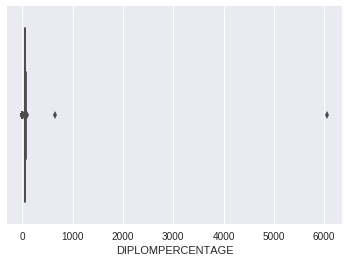
\includegraphics[width=0.5\textwidth]{fig/AGEPlot1.png}
	\caption[Short caption]{Box Plot Attribue Diplôme Pourcentage  }
	\label{fig:AgeBXPlot1}
\end{figure} 

\begin{figure}[ht]
	\centering
	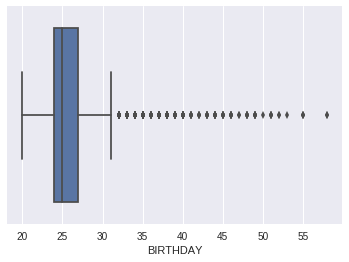
\includegraphics[width=0.5\textwidth]{fig/PercetagePlot.png}
	\caption[Short caption]{Box Plot Attribue  Age  }
	\label{fig:PercBXPlot1}
\end{figure} 
Au vu de ces courbes nous remarquons que l'attribue diplôme pourcentage
dispose de beaucoup des déviations. Nous avons pu corriger au cas par cas en remplaçant les valeurs aberrantes par leurs valeurs exactes et d'autres par la moyenne comme il n'était pas nombreux
\subsubsection{Données mal orthographiées }
Dans notre première analyse nous avons remarqué que certaines  attribues ont des valeurs très désorganisées et vraiment dispersé et ce
qui a une mauvaise influence sur le calcul de l'entropie et ainsi sur
les algorithmes du Machine Learning . Nous pouvons aisément constater
que ce problèmes est du à des fautes d'orthographes commise lors de la
phase de saisie des données et ainsi pour continues nous devons essayer
de corriger ces erreurs et bien organisé les données . 

Par exemple pour la variable diplôme section on a pu voir les valeurs suivantes : 'TECSC', 'Techniqe',
'TECHN IQUE',technique','TCH' qui sont saisie pour la même et unique
section 'techniques' mais avec différentes erreurs d'orthographe. \\
Pour l'attribut SCHOOL nous avons obtenus les valeurs suivantes :
'matanoia', 'metanoia', 'metonoina', '\%etanoia', 'meta' pour la seule école 'metanoia'
Nous avons aussi remarqué ces genres d'incohérence pour les autres attribues catégorielles.  
Après analyse nous avons pu détecter qu'il étaient  du à des erreurs d'orthographe.
Ces genres d'erreur de notation ont pour conséquence le fait qu'il font
augmenter l'entropie de nos colonnes et ainsi pénalisent nos algorithmes
surtout lorsqu'on travaille avec les arbres de décisions .Nous avons
procédé à un nettoyage automatique qui a consisté en un groupement des
valeurs proches en utilisant la distance de Leveinstein :\cite{LevStack}combinée au  clustering par l'algorithme d'affinity propagation,et
ainsi qu'un nettoyage manuelle pour arranger les données à la fin de
cette phase nous avons obtenus des données moyennement propres et bien
nettoyer avec un entropie faible.
 \subsection{Analyse des données}\label{analyse-des-donnuxe9es}
\paragraph{}
Cette phase comprend une analyse statistique bi-varié et uni-varié nous
visualiserons les résultat à l'aide des graphiques . Dans cette partie
nous utiliserons beaucoup plus la statistique descriptives et la statistique inférentielle
Comme nous  pouvons le remarquer notre ensemble d'apprentissage
comprend à la fois des données numériques (continues ) ainsi que des
données discrètes catégories. voici comment nous allons procéder

\subsubsection{Analyse Uni-Varié}
Dans cette partie nous allons effectuer les statistiques descriptives pour chaque variable .
\begin{enumerate}
	\item
	\emph{\textbf{Variable Numériques ou continues : }}Pour les données continues nous
	allons essayer de comprendre la tendance et la dispersion des nos
	variables .les métriques utilisées sont sur la figure suivante: 
	\begin{figure}[ht]
		\centering
		\includegraphics[width=0.5\textwidth]{fig/DataExploration.png}
		\caption[Short caption]{Techniques d'exploration des données en entré }
		\label{fig:DataExplora}
	\end{figure}
	En bref nous allons examiner le moyenne , le mode , l'écart-type et la
	variance , nous conterons aussi les variables nous allons faire les
	visualisations avec des box-plot! cette étape nous sera aussi utile
	dans le traitement des valeur manquantes et des valeurs aberrantes!
	\item
	\emph{\textbf{Variable catégorielle ou quantitative :}} Pour les données discrètes nous
	allons utiliser  les tables des fréquences pour comprendre la distribution de
	chaque catégorie nous pour aussi voir le pourcentage de chaque
	catégorie , les histogrammes et bar char seront utilisées.
\end{enumerate}
Commençons par l'analyse des attributs numériques age et pourcentage à l' \ac{EXETAT} 
\paragraph{L'AGE et Le Diplôme Pourcentage}
Voici un bref aperçu des statistiques descriptives de ses variables  à la la figure la figure \ref{tab:DescribeData}
\begin{table}
	\centering
	\begingroup % make the next setting local
	\captionsetup{type=table} % here we want to caption a table
	\caption{Statistiques Des Données }
	\label{tab:DescribeData}
	\begin{tabular}{lrr}
		\toprule
		{} &  DIPLOMPERCENTAGE &          AGE \\
		\midrule
		count &       4715,000000 &  4715,000000 \\
		mean  &         56,878914 &    24,732768 \\
		std   &          5,756663 &     4,621602 \\
		min   &         50,000000 &    18,000000 \\
		25\%   &         52,000000 &    22,000000 \\
		50\%   &         56,000000 &    24,000000 \\
		75\%   &         60,000000 &    27,000000 \\
		max   &         86,000000 &    59,000000 \\
		\bottomrule
	\end{tabular}
\endgroup
\end{table}
\subparagraph{AGE}

Nous avons calculer l'age en se basant sur la date de naissance et la date d'aujourd'hui.signalons que cet attribue disposait des valeurs manquantes au début et on était imputer par la moyenne , comme nous pouvons le voir à la la figure la figure \ref{tab:DescribeData}  nos étudiant disposent en moyenne d'un age de 24 ans avec une variance de 4,5 le moins âgé a 18 ans et le plus âgé a 59 ans.
On peut aisément que l'age suit une distribution normale . 
\begin{figure}[!htbp]
	\centering
	\subfloat[Box-Plot ad l'age ]{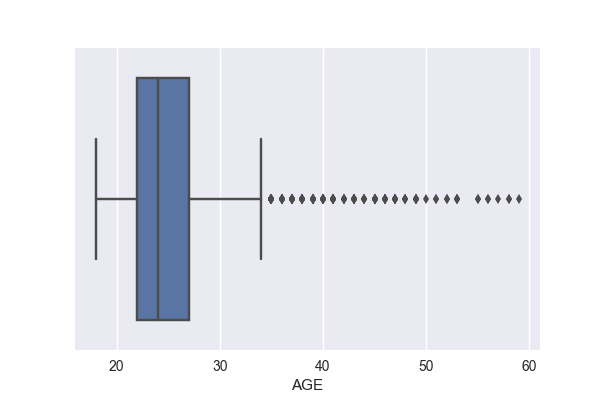
\includegraphics[width=0.4\textwidth]{fig/AGE.png}\label{fig:Agea}}
	\hfill
	\subfloat[distribution de l'age ]{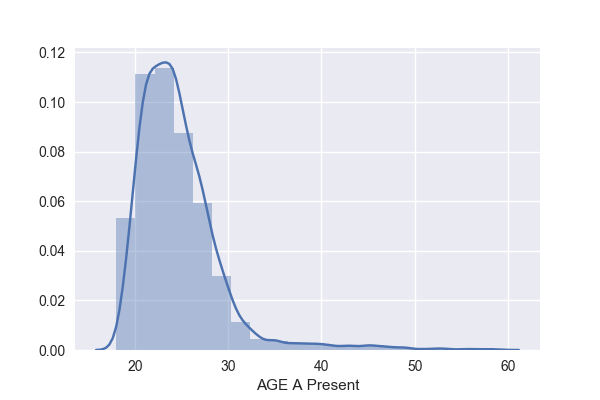
\includegraphics[width=0.4\textwidth]{fig/AGEDist.png}\label{fig:Ageb}}
	\hfill
	\caption{Graphiques de l'attribue age}
\end{figure}
\subparagraph{Pourcentage du diplôme}
Après nettoyage et contrairement à la la figure la figure \ref{tab:MisisnV} on a constater qu'après nettoyage la moyenne est de 56,8 \% avec unn écart type de 5,7 le minimum de 50 \% et un maximum de 86\% .
les graphiques représentent les informations sur l'age  son à la la figure la figure \ref{fig:Pourcentagea} et la figure la figure \ref{fig:Pourcentageb}
\begin{figure}[!htbp]
	\centering
	\subfloat[Box-Plot du Pourcenatge du diplome ]{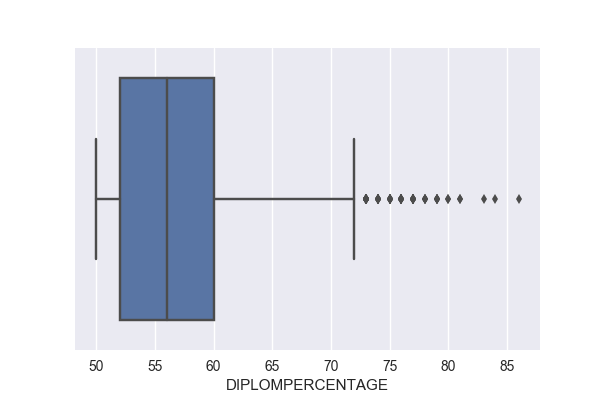
\includegraphics[width=0.4\textwidth]{fig/dipomePourcentage.png}\label{fig:Pourcentagea}}
	\hfill
	\subfloat[distribution du Pourcenatage ]{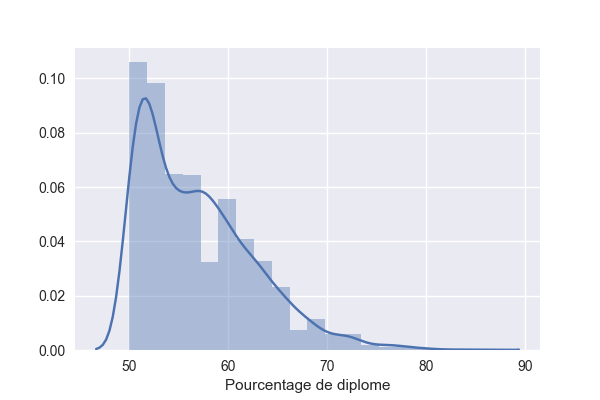
\includegraphics[width=0.4\textwidth]{fig/diplomePercentageDis.png}\label{fig:Pourcenategb}}
	\hfill
	\caption{Graphiques de l'attribue du Pourcentage à l'examen d'état }
\end{figure}
\subparagraph{Le Sexe des étudiants}
	\begin{figure}[!htbp]
	\centering
	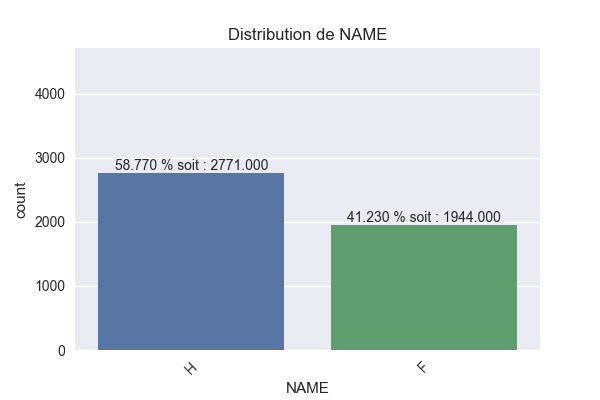
\includegraphics[width=0.5\textwidth]{fig/NAME.png}
	\caption[Short caption]{Distribution du sexe des étudiants }
	\label{fig:SEXE}
\end{figure}
La  la figure la figure \ref{fig:SEXE} nous donne la  répartition de sexes dans notre ensemble d'apprentissage on peut aisément constater qu'il n'est pas si déséquilibre que ça!, le
genre est vraiment respecté avec 41\% dés nouveaux étudiant étant de
sexe féminin.
\subparagraph{le type d'école}
\begin{figure}[!htbp]
	\centering
	\makebox[\textwidth]{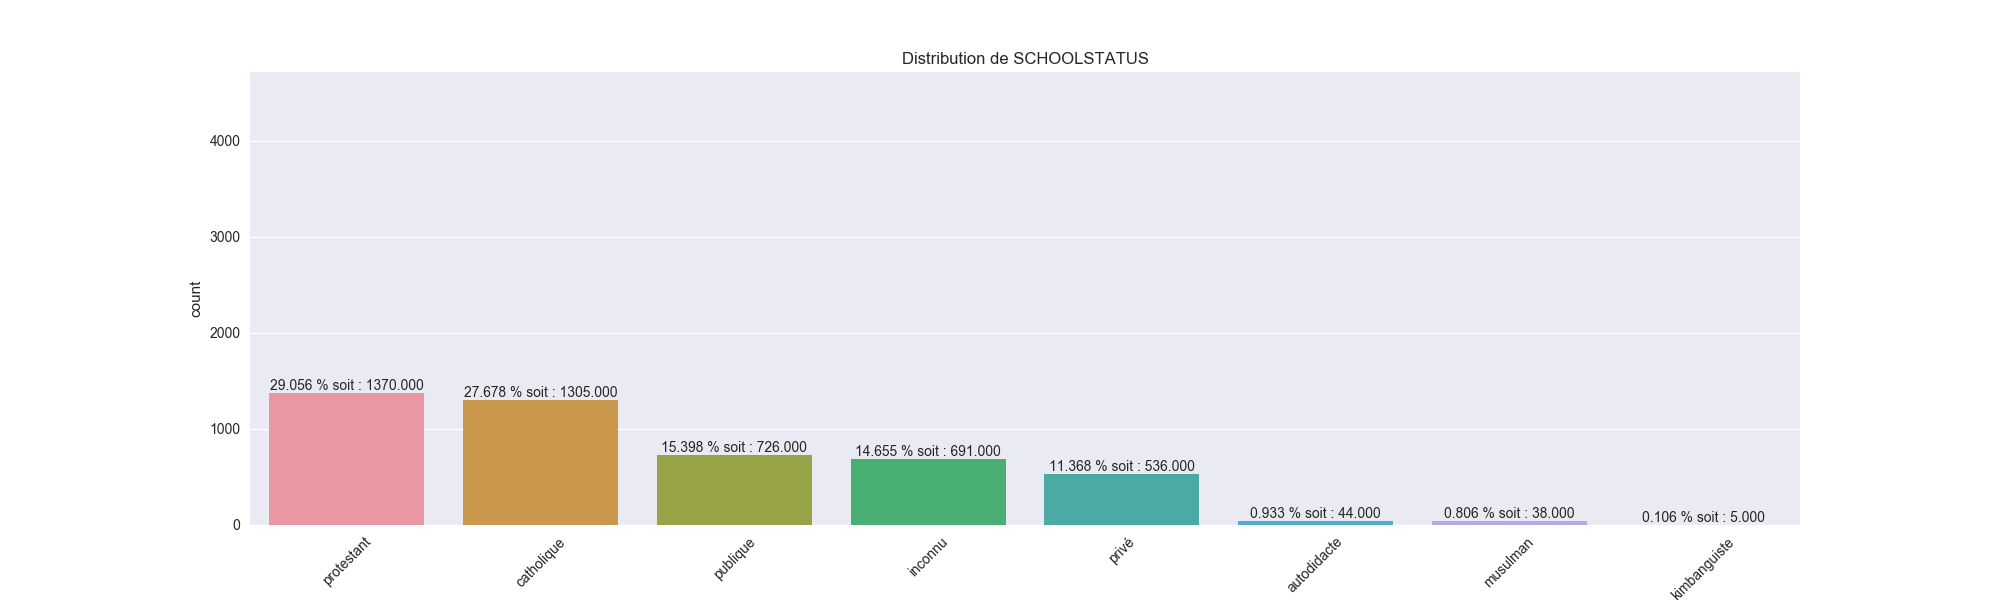
\includegraphics[width=\paperwidth]{fig/SCHOOLSTATUS.png}}
	\caption[Short caption]{Différente statut de l'école de provenance }
	\label{fig:SchoolStatus}
\end{figure}
 Dans la la figure la figure \ref{fig:SchoolStatus} nous pouvons remarquer aisément que 29\% des étudiants
proviennent des écoles dites protestantes , 27\% viennent des écoles
catholiques , 11\% des écoles privé , 15 des écoles publiques mais aussi
il ya des étudiants venant des autodidactes , ceux provenant des écoles
musulmanes et kibanguistes mais en proportion vraiment négligeable.
\subparagraph{l'Option de provenance}
Nos étudiant Proviennent des 33 écoles différentes:

\begin{figure}[!htbp]
	\centering
	\makebox[\textwidth]{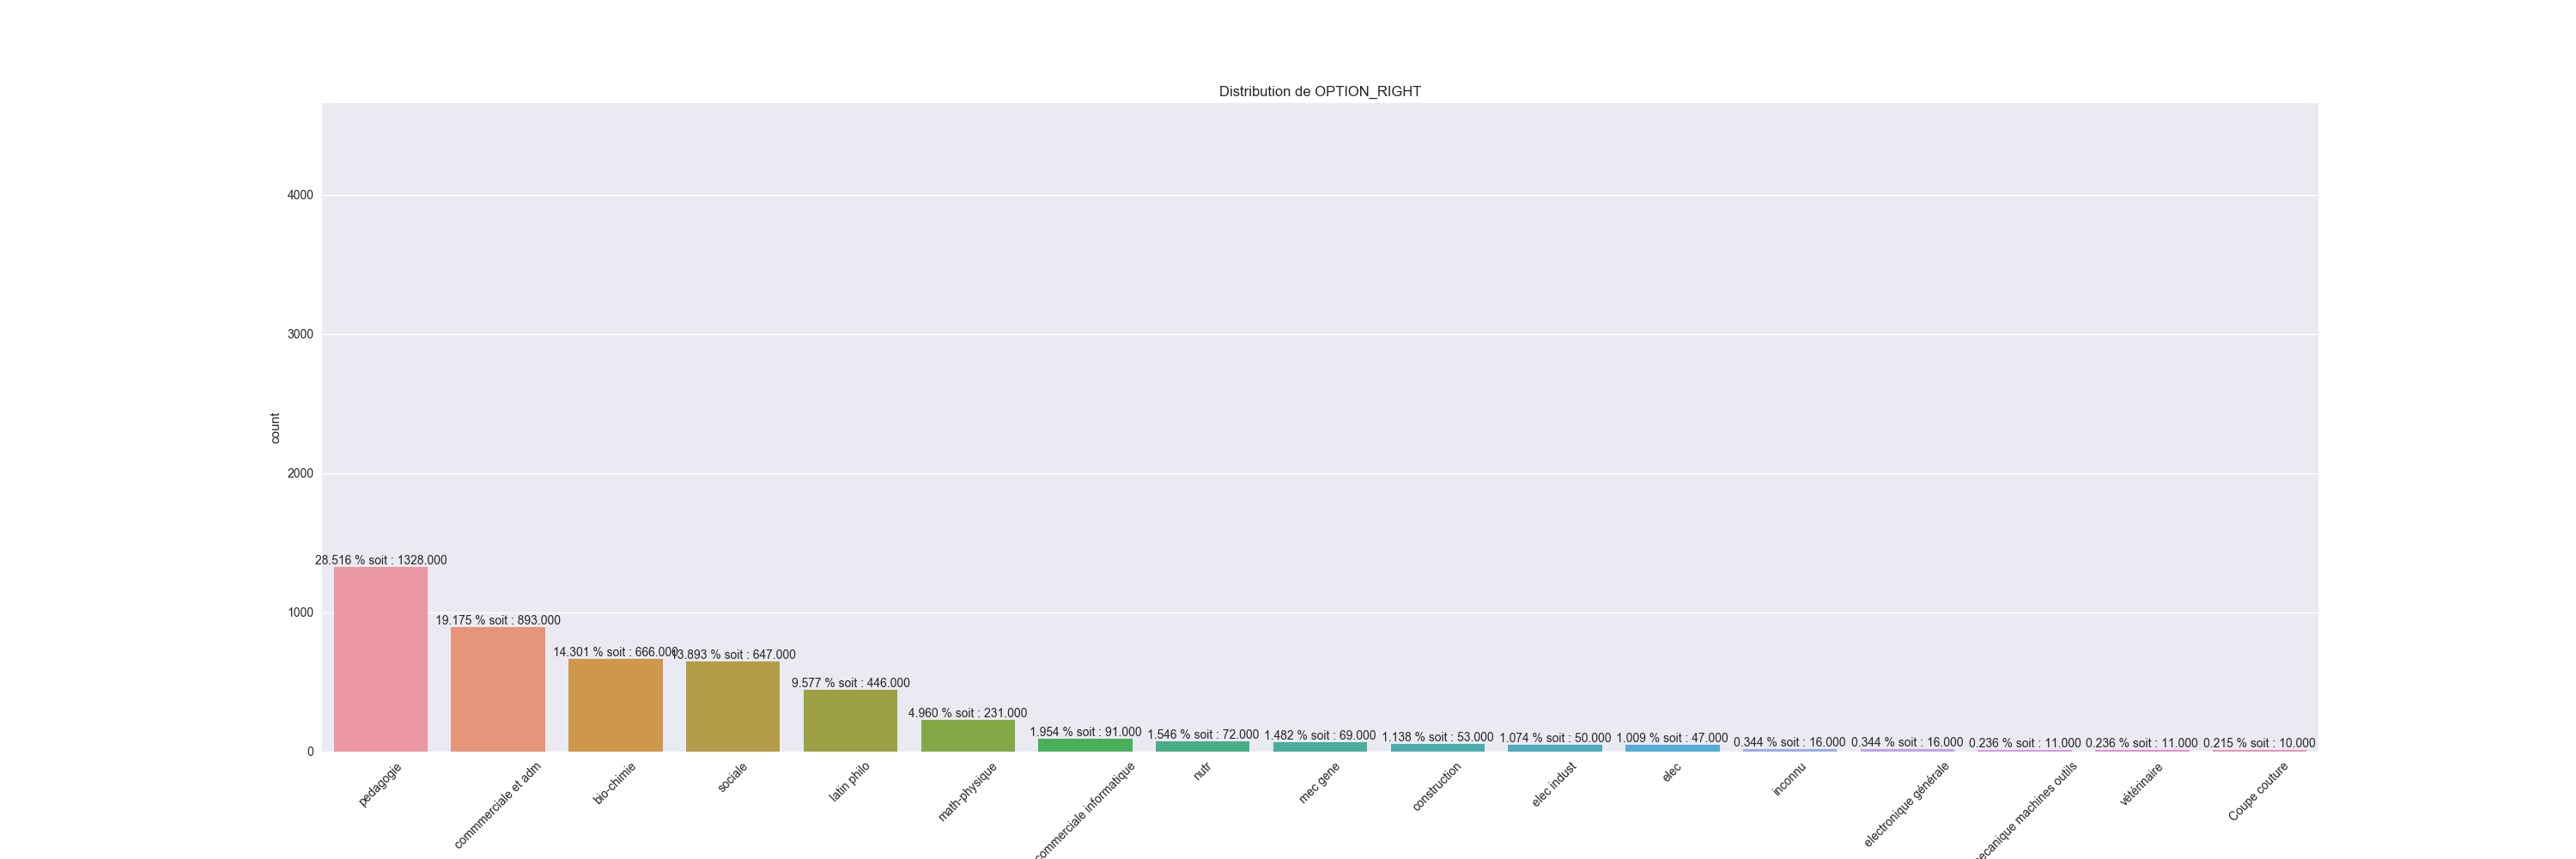
\includegraphics[width=\paperwidth]{fig/OPTION_RIGHT.png}}
	\caption[Short caption]{l'option suivie à l'école secondaire }
	\label{fig:Option_right}
\end{figure}
Sur la la figure la figure \ref{fig:Option_right} nous pouvons remarquer que la majeure partie des
étudiants de notre études proviennent de la section pédagogique avec
environ 28\% ensuite vienne la section commerciale et administrative
avec 19\% , suivent sociale avec 13\%, scientifique bio-chimie avec 14
\% ensuite viennent autres différentes options avec des valeurs
inférieurs à 5\%.
\subparagraph{Attribut School}\label{attribut-school}
cette attribue comprend les valeurs de l'école de provenance des nos
finaliste combiné avec l'attribue SCHOOLSTATUS  il joue un rôle
important dans notre étude.
nous pouvons aisément remarquer que les élèves proviennent de 594 écoles
différentes sur la figure \ref{fig:SCHOOL} nous allons visualiser les écoles
les plus représentées.
\begin{figure}[!htbp]
	\centering
	\makebox[\textwidth]{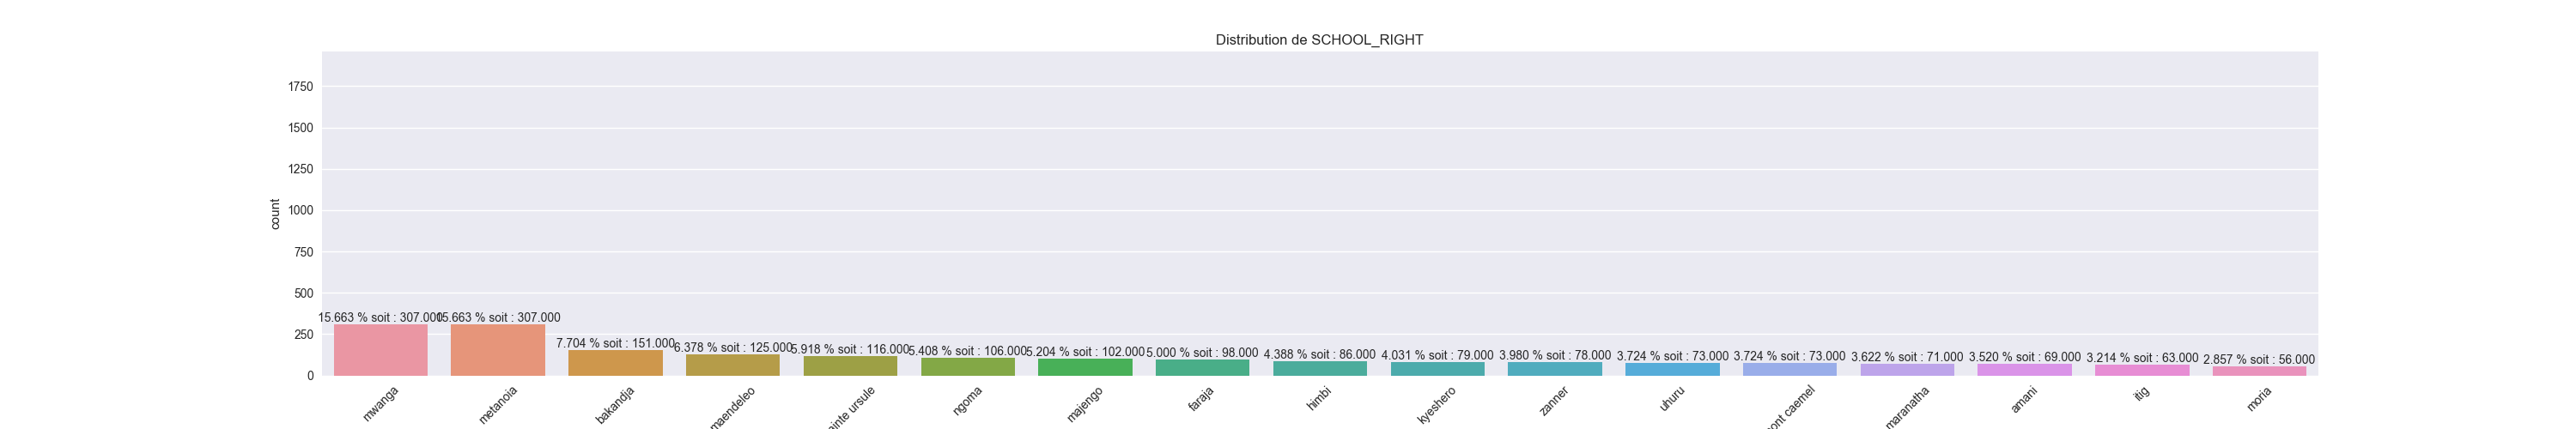
\includegraphics[width=\paperwidth]{fig/SCHOOL_RIGHT.png}}
	\caption[Short caption]{les écoles de provenances  }
	\label{fig:SCHOOL}
\end{figure}
Nous pouvons remarquer aisément que le top 10 des école de provenance
est constituer de grandes écoles de la ville de Goma avec l'institut
metanoia et le collège mwanga en tête de liste avec l'institut mwanga et
metanoia en tete de liste avec 15\% chacun ensuite vienne l'institut
bakanja avec 6\% ensuite vienne maendelo, le lycée sainte ursule et
l'institut de Goma avec 6\%, 5\% et 5 \% respectivement et d'autres
école se partagent le reste de 50\%.
\subparagraph{Attribue SCHOOL Province}
\begin{figure}[!htbp]
	\centering
	\makebox[\textwidth]{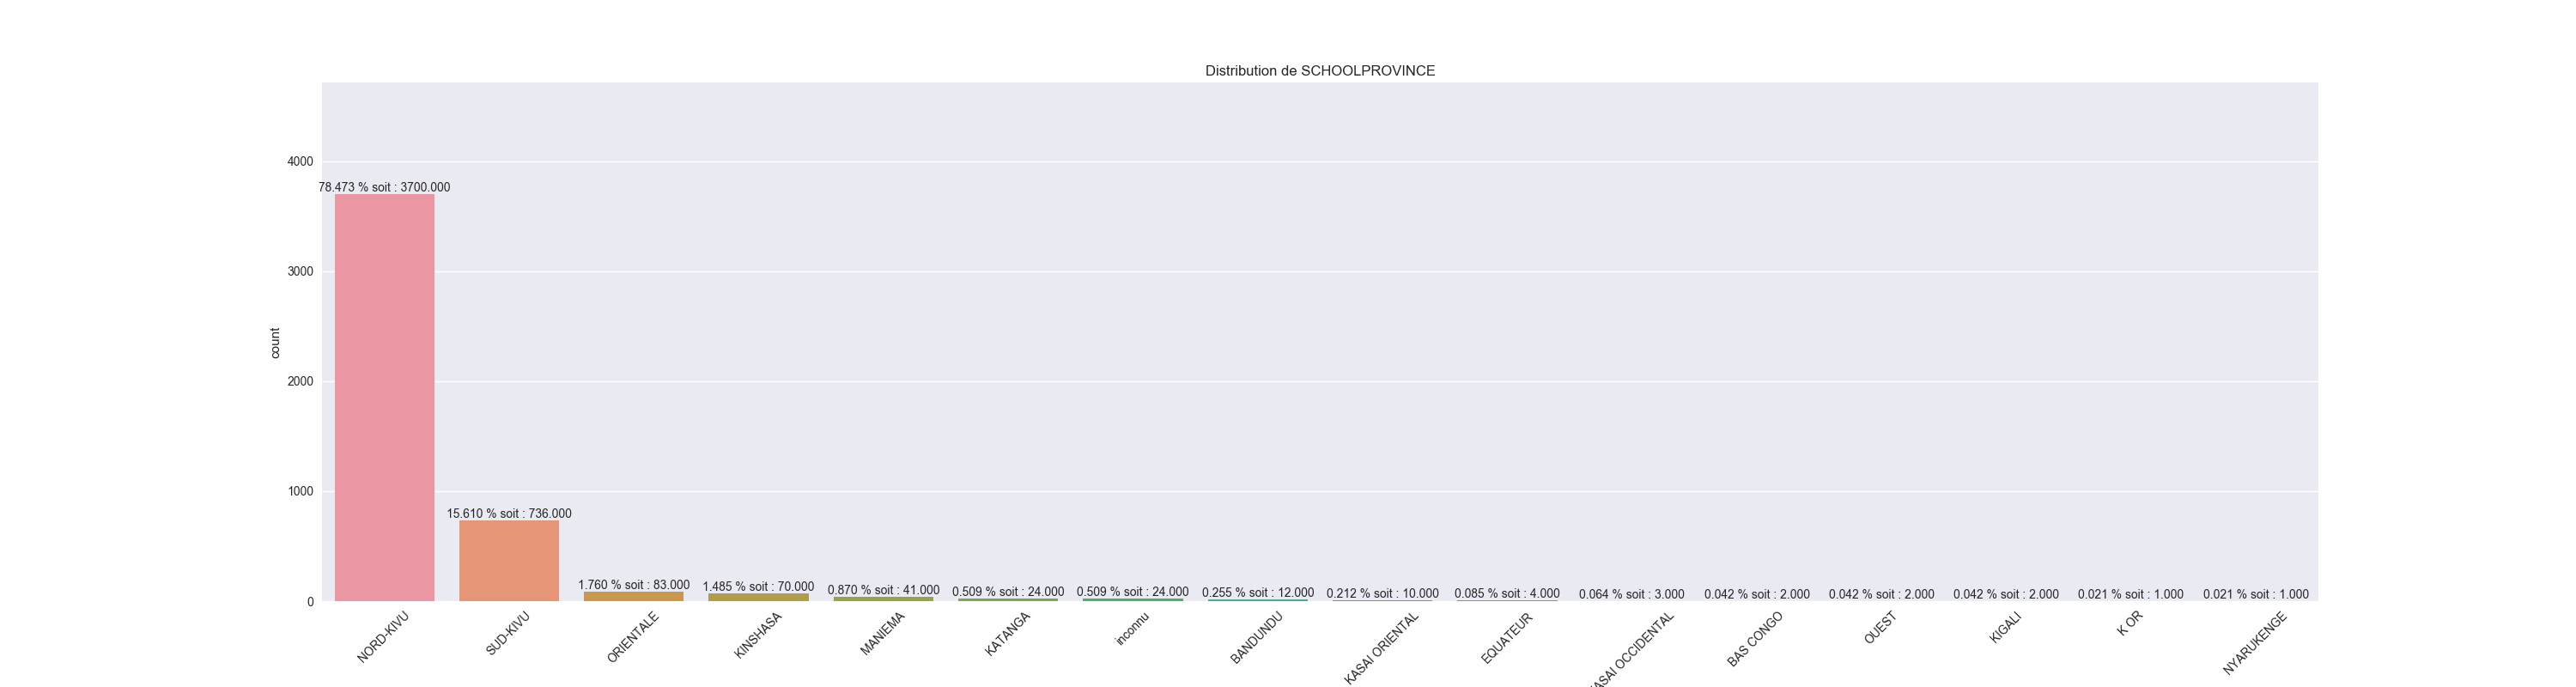
\includegraphics[width=\paperwidth]{fig/SCHOOLPROVINCE.png}}
	\caption[Short caption]{les provinces de provenances des étudiants   }
	\label{fig:SCHOOLProvince}
\end{figure}
A la figure \ref{fig:SCHOOLProvince} nous pouvons aisément constater que 75 \% des étudiants
de l'\ac{ULPGL} proviennent de la province du nord kivu mais il ya une autre
catégorie provenant  du Sud Kivu soit 15\% l'autre partie provient des autres provinces de la \ac{RDC}.
\subparagraph{Attribue Faculté}
Pour finaliser l'analyser uni-varié des nos données en entrée nous allons jeter un coup d'œil sur la colonne Fac qui contient la faculté choisie par l'étudiant.
Voici comment elle se présente a la figure \ref{fig:FAC}:
\begin{figure}[!htbp]
	\centering
	\makebox[\textwidth]{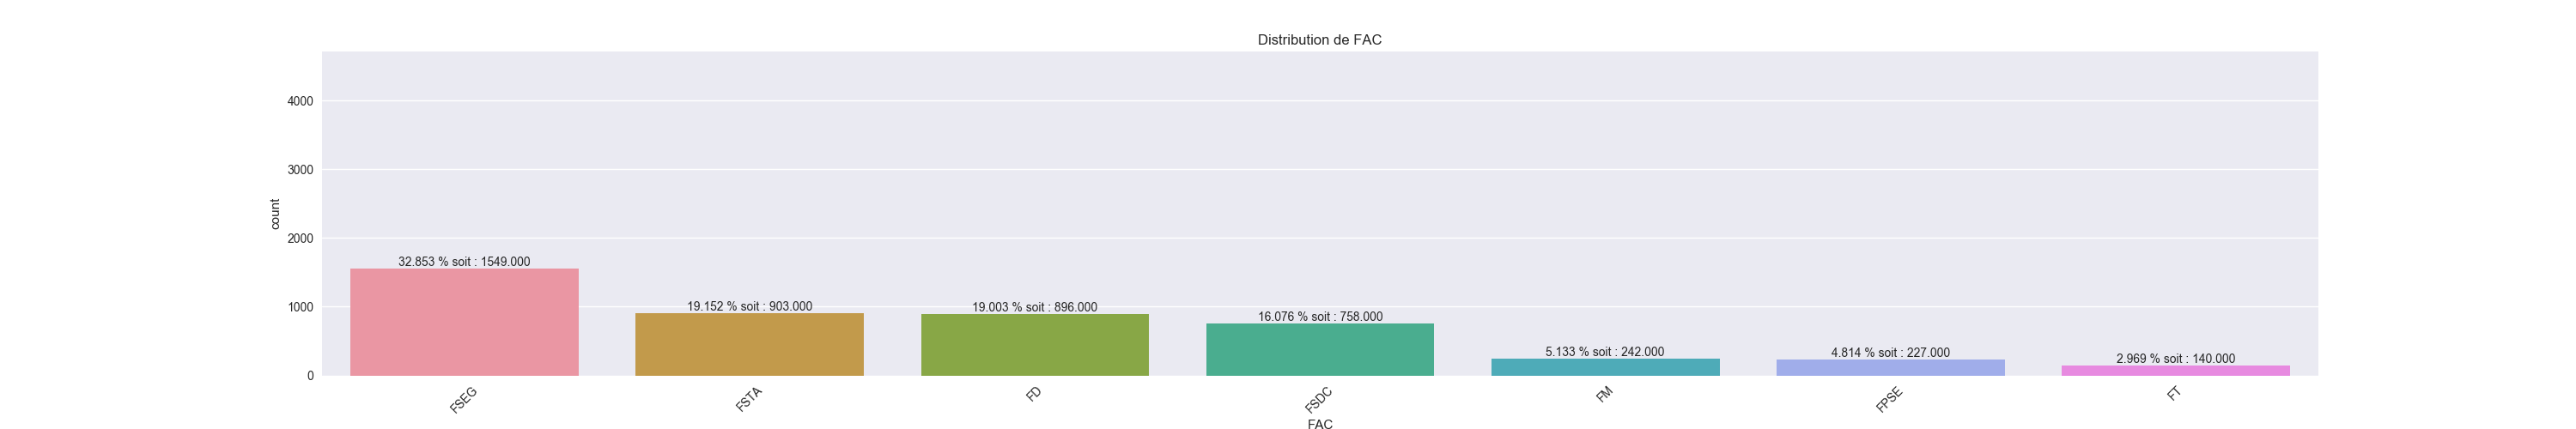
\includegraphics[width=\paperwidth]{fig/FAC.png}}
	\caption[Short caption]{les FAculteé}
	\label{fig:FAC}
\end{figure}
 Nous remarquons la distribution des valeurs pour
l'attribue faculté des étudiants: - FSGEG: 32,8\% , FSTA : 19,153\% , FD
:19\% -,FSDC :16\% ,FM : 5\% ,FPSE : 4\% ,FT :3\%
\subsubsection{Analyse Bi-variée}
C'est une technique d'analyse statistique des données, consistant à
découvrir la relation pouvant exister entre 2 variables dans le but de
tester l'hypothèse d'association et de causalité entre 2 variables !Par
exemple dans notre analyser nous allons essayer de voir la relation
existant entre le choix de la faculté et le pourcentage du diplôme à l'examen d'état. Elle se déroule en 4 étapes : \cite{becker2011uncertainty}
\begin{itemize}
	\item Définition de la nature des relations
	\item  identification et direction des relations 
	\item   Détermination si
	la relation est important du point de vue statistique(Intervalle de
	confiance)
	\item  Détermination si
	la relation est important du point de vue statistique(Intervalle de
	confiance)
\end{itemize}
Nous effectuerons cette analyse à 3 niveau :
\begin{enumerate}
	
	\item
	\emph{\textbf{Variables Continues et
			catégorielle ou quantitatives: }}
	Pour effectuer cette analyse nous
	utiliserons le test \ac{ANOVA},
	c'est une technique statistique permettant de comparer les moyennes de plus de deux populations. Son but est en fait de procéder à une sorte de généralisation de la comparaison des moyennes ou de la comparaison des pourcentages lorsqu'il y a plus de deux valeurs à comparer. Il s'agit aussi de l'équivalent, pour des variables qualitatives de la régression linéaire.
	\paragraph{}
	Cette technique est utile en sciences sociales dans l'analyse de certaines données, organisées en blocs de même taille. Il s'agit dans ce cas le plus souvent d'analyse de la variance à un seul facteur. Les analyses à deux facteurs sont en revanche fréquentes dans l'exploitation d'enquêtes d'usage psychologique.
	\paragraph{}
	Les données de notre étude répondent bel et bien à l'usage de la technique de l'Analyse de la variance. Ainsi, à travers les pages qui suivent, nous analysons l'effet des variables  Age, pourcentage à l'examen d'état, sur l'option choisie par l'étudiant . Par la même occasion nous nous permettons de comparer des histogrammes de chaque groupe en fonction des mêmes variables ; ainsi que les divers seuils de significative.
	\paragraph{}
	Pour cette analyse l'hypothèse nulle est du type:
	H0 : les moyennes sont égales dans toutes les catégories. 
	et son hypothèse alternatif est 
	H1 : au moins une moyenne est différente des autres..
	\item \emph{\textbf{Variable catégorielle ou catégorielle  :}} 
	Pour ces types des données nous allons effectué le test de chi-carré: Le chi-carré est un test statistique conçu pour déterminer si la différence
	entre deux distributions de fréquences est attribuable à l'erreur
	d'échantillonnage (le hasard) ou est suffisamment grande pour être
	statistiquement significative.
	Ho - est, comme son nom l'indique, une hypothèse qui postule qu'il n'y a pas de différence entre les fréquences ou les proportions des deux groupes elle est considéré comme hypothèse nulle.
	Si la différence entre les deux distributions est réduite, l'hypothèse
	nulle sera acceptée. Si la différence est grande, l'hypothèse nulle sera
	rejetée. Dans ce dernier cas, on parlera d'une différence
	statistiquement significative parce que l'écart entre les deux
	distributions est trop important pour être expliqué par le hasard
	seulement : une différence réelle existe donc.
\item \emph{\textbf{Variable continues et continues  :}} 
Pour les variables continues on utilise cherche la corrélation et pour
notre travail nous allons utilisée le coefficient de corrélation de
Pearson: Les coefficients de corrélation permettent de donner une mesure
synthétique de l'intensité de la relation entre deux caractères et de
son sens lorsque cette relation est monotone. Le coefficient de
corrélation de Pearson permet d'analyser les relations linéaires et le
coefficient de corrélation de Spearman les relations non-linéaires
monotones. Il existe d'autres coefficients pour les relations
non-linéaires et non-monotones.
Signalons que python dispose des multiples librairies pour effectuer ces
genres d'analyse et nous les utiliserons dans la suite
\end{enumerate}\cleardoublepage
\chapter{Élaboration  et évaluation du modèle de prédiction }
Tous au long de ce chapitre nous allons entrainer nos algorithmes de prédiction avec des données provenant de chaque faculté et essayerons de prédire le CGPA, nous  avons utiliser des algorithmes présenté au chapitre premier pour entrainer nos modèles de prédiction.
Pour choisir l'algorithme à utiliser nous somme basée sur la documentation officielle de la librairie scikit-learn \cite{pedregosa2011scikit} qui nous a fourni l'infographie sur la figure \ref{fig:skLearn1} pour le choix des algorithmes. \\

\begin{figure}[ht]
	\centering
	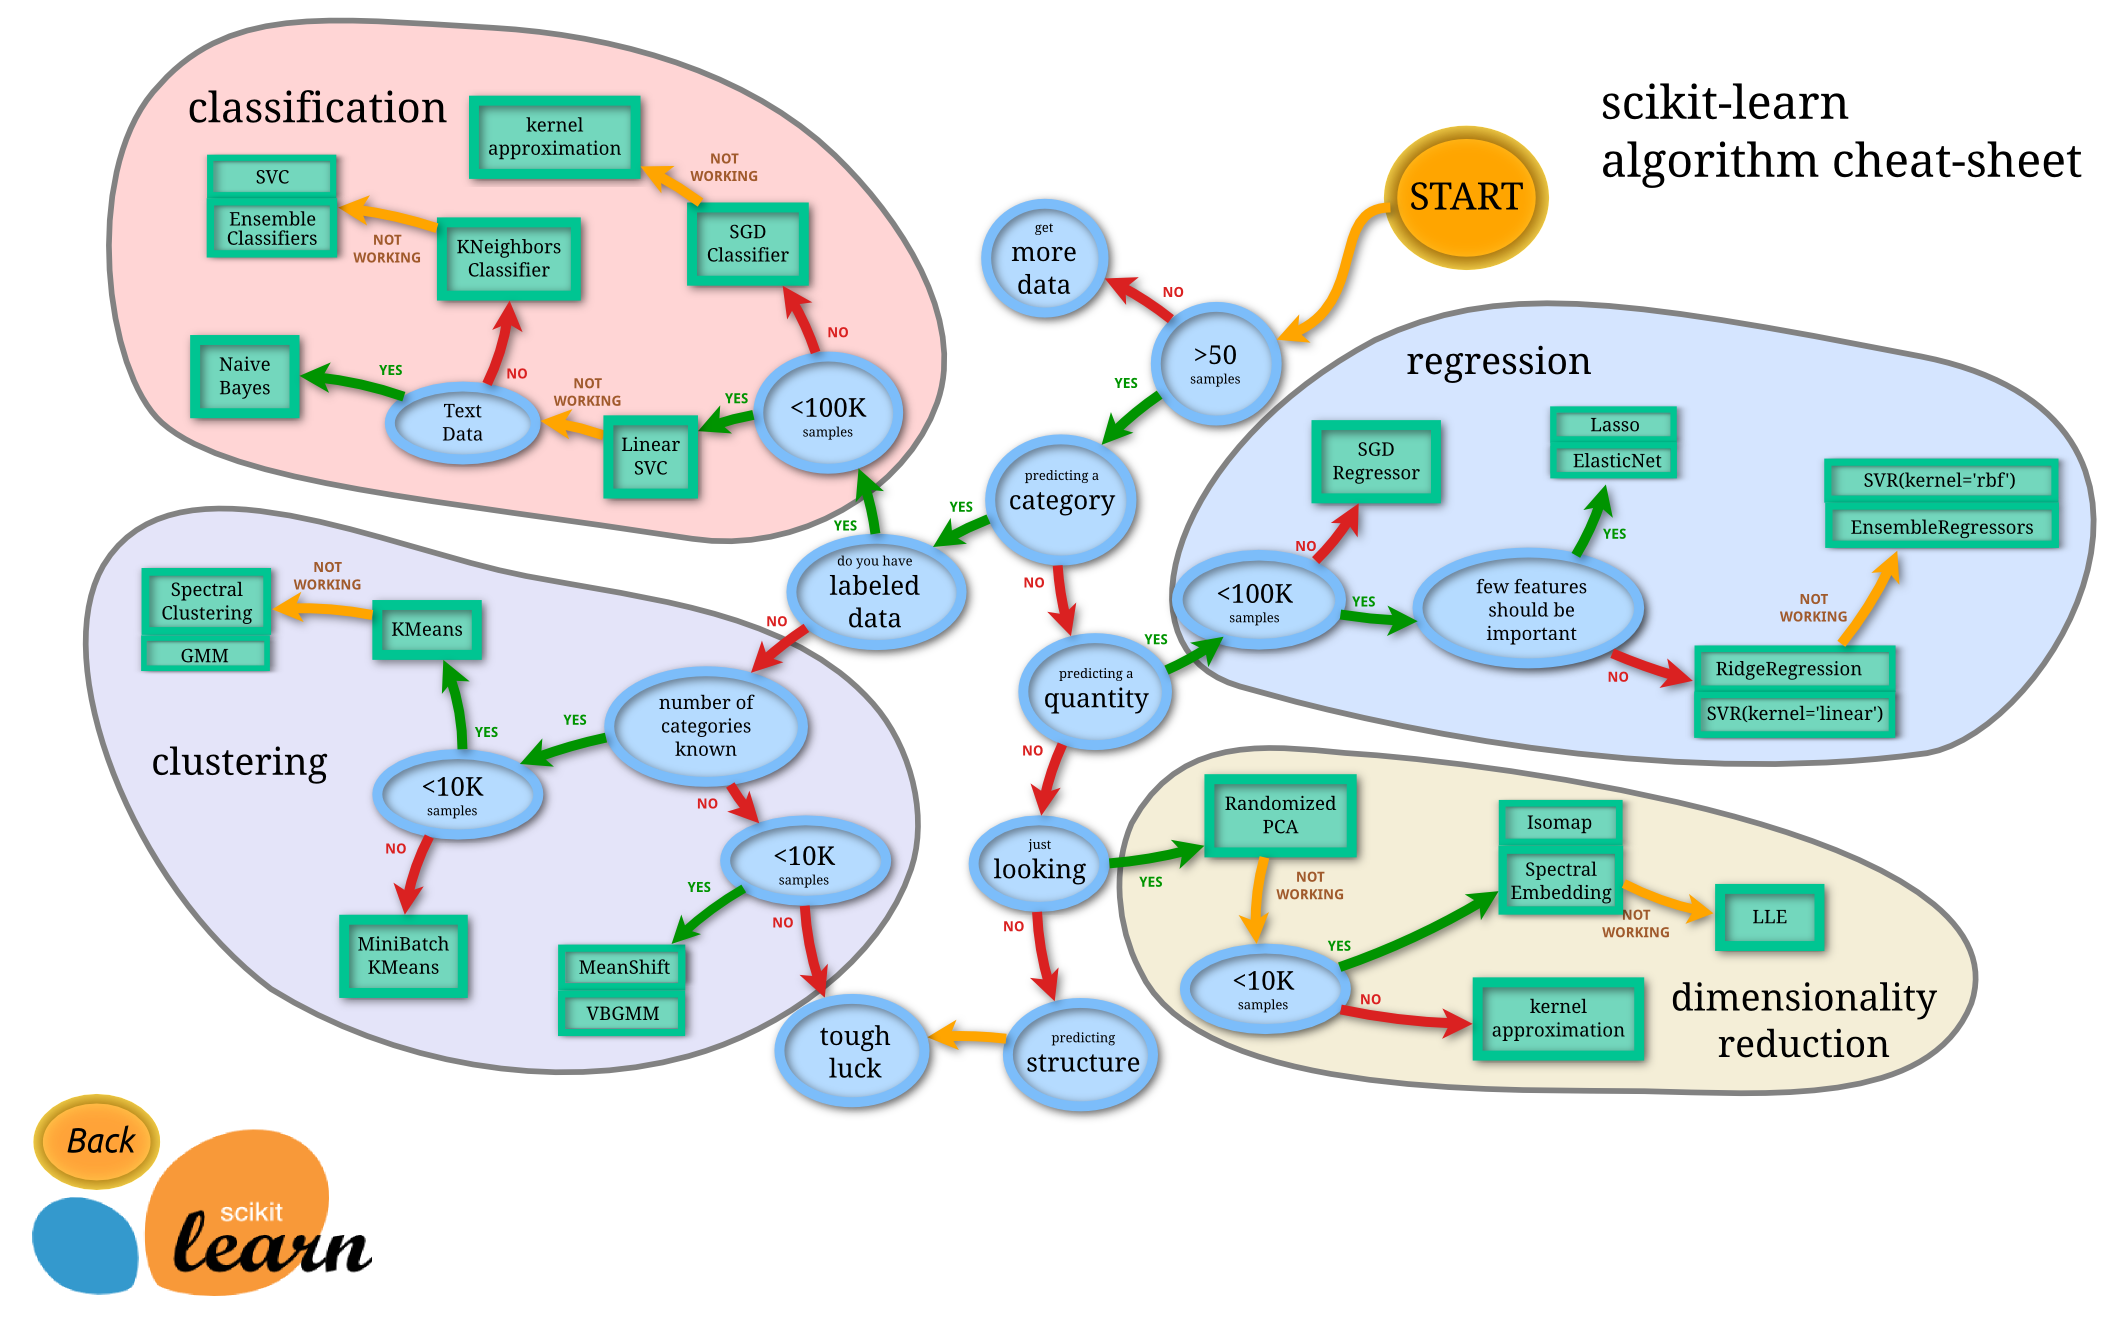
\includegraphics[width=0.5\textwidth]{fig/sckikLearnCheatSheet.png}
	\caption[Short caption]{sckit-Learn Algorithm cheat sheet }
	\label{fig:skLearn1}
\end{figure} 

Vu que nous disposons de moins de 100000 instances pour nos ensemble d'apprentissage et vu que notre tache était celui de prédire une variable continue (Une régression )  nous avions décidé d'entrainer les algorithmes  suivantes :
\begin{enumerate}
	\item Ridge Régression
	\item Elastic Net Régression
	\item Lasso Régression
	\item \ac{SVR} avec Kernel Linéaire
	\item  \ac{SVR} avec Kernel Gaussien 
\end{enumerate}
Les 3 premiers modèles sont des versions issues de la régularisation de la régression linéaire vu au chapitre 1  et qui conviennent bien pour des ensembles d'apprentissages relativement petits , le 2 derniers sont une adaptation du \ac{SVM} pour la régression.\\
Notons que toutes ses librairies sont bien implémentées et optimisées dans scikit-learn.
Tous au long de ce chapitre nous avions suivie les étapes suivantes  sur la figure \ref{fig:predictiveModelBuilding}:
 \begin{enumerate}
 \item Préparation des données :
 \begin{itemize}
 	\item  Encodage One Hot
 	\item  Normalisation
 	\item  Échantillonnage
 \end{itemize}
\item Exécution des algorithmes
\item évaluation 
   \begin{itemize}
  	\item  Évaluation sur l'ensemble d'apprentissage (training set)
  	\item  Validation croisée sur l'ensemble d'apprentissage
  	\item  Évaluation sur l'ensemble d'évaluation (test set) 
  \end{itemize}
\item Amélioration des modèles par les méthodes d'ensembles
\item Évaluation du modèle finale
 \end{enumerate}
\begin{figure}[ht]
	\centering
	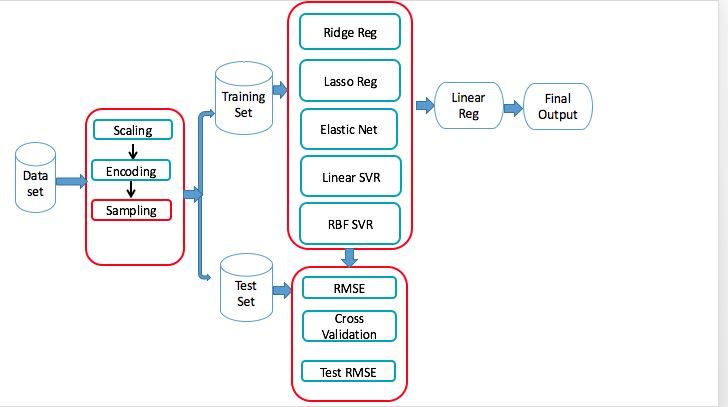
\includegraphics[width=0.5\textwidth]{fig/ModelBuilding.png}
	\caption[Short caption]{étapes à suivre pour l'élaboration du modèle d'apprentissage }
	\label{fig:predictiveModelBuilding}
\end{figure} 
\section {Préparation des données pour l'exécution des algorithmes } 
Dans cette partie nous expliquerons comment s'est passé la préparation des nos données , rappelons que notre ensemble d'apprentissage finale dispose de 4 attribues et notre valeur à prédire :
\begin{enumerate}
	\item  SCHOOLNAME : de nature catégorielle (string)
	\item  OPTION : de nature catégorielle (string)
	\item  DIPPERC : de nature continue (float)
	\item  CGPA : de nature continue (float)
\end{enumerate}
Comme l'a souligné \cite{OneHotEncoding} la librairie scikit learn ne travaille qu'avec les variables numériques , c'est pourquoi nous avions décider de transformer nos variables catégorielles les chaines de caractères en variables numériques en utilisant la technique du \emph{\textbf{One Hot encoding}} 
\subsection{Encodage des Variables One Hot }
Un encodage one-hot consiste à représenter des états en utilisant pour chacun une valeur dont la représentation binaire n'a qu'un seul chiffre 1.

On peut définir une fonction d'encodage one-hot comme étant la fonction qui prend en entrée un vecteur  z et qui redéfinit en sortie la plus grande valeur de  z à 1 et toutes autres valeurs de  z à 0.
L'avantage principal de cet encodage est que pour passer d'un état à un autre, seules deux transitions sont nécessaires : un chiffre passe de 1 à 0, un autre de 0 à 1. Son inconvénient est qu'il faut au minimum n bits pour représenter n états, ce qui conduit à une augmentation linéaire du nombre de chiffres par rapport au nombre d'états. Un encodage utilisant toutes les valeurs binaires existantes a quant à lui une augmentation logarithmique du nombre de chiffres.

Pour notre ensemble , après notre encodage nous pouvons aisément remarquer que notre ensemble d'apprentissage vient de passer de (4715, 4 )à (4715 , 647)  dimensions.
Mais ces dimension restent raisonnables pour un projet de machine Learning. 
\subsection{Normalisation  } 
Nous avions ensuite normaliser nos données pour les variables numérique en divisant le pourcentage du diplôme d'état par 100 et celui du CGPA,ceci pour permettre une exécution rapide de nos algorithmes. 
\subsection{Échantillonnage  \cite{statBook1} } 
Pour commencer notre entrainement nous avions échantillonner nos donnes pour constituer un ensemble d'apprentissage (Training set), et un ensemble d'évaluation du modèle (test set). Notre Training set était constituer de 80 \% de nos données et les 20 autres pour cent ont constitué notre ensemble d'évaluation.
Pour ce faire nous avions utilisé un échantillonnage stratifié.
Lorsqu'on utilise l'échantillonnage stratifié, on divise la population en groupes homogènes (appelés strates), qui sont mutuellement exclusifs, puis on sélectionne à partir de chaque strate des échantillons indépendants. On peut utiliser n'importe quelle des méthodes d'échantillonnage  pour sélectionner l'échantillon à l'intérieur de chaque strate. La méthode d'échantillonnage peut varier d'une strate à une autre. Lorsqu'on utilise l'échantillonnage aléatoire simple pour sélectionner l'échantillon à l'intérieur de chaque strate, on appelle le plan d'échantillonnage un plan d'échantillonnage aléatoire simple stratifié. On peut stratifier avant l'échantillonnage une population au moyen de toute variable dont on dispose pour la totalité des unités , pour notre étude nous avions utilisé la variable \textbf{EchecRatio}.

A la fin de cette phase nous avions pu obtenir un ensemble d'apprentissage (Training Set) et Un ensemble d'évaluation (Test Set )

\section {Élaboration et Évaluation du Modèle de Prédiction au sein de Chaque faculté} 
Dans cette section nous allons entrainer les différents algorithmes de prédictions avec les données de issue de chaque faculté et ensuite nous évaluerons le modèles sur les 2 ensemble.

Mais avant d'attaquer l'entrainement de nos modèle nous expliquerons nos métriques d'évaluations.
\subsection{Techniques D'évaluation} 
\subsubsection{\ac{RMSE} \cite{ProbaStat} }
C'est la racine carrée de la somme des carrées des différences entres les valeurs exactes et celles prédite par un modèle de prédiction pour chaque élément d'un ensemble d'apprentissage .
Il se donne par la formule suivante  :

 $RMSE=\sqrt{\frac{\sum _{=1}^{N}{\left[{h}_{\theta}\left({x}^{(i)}\right) - {y}^{(i)}\right]}^2} {N}}$
 
 Il constituera notre métrique d'évaluation pour tous nos modèles.
\subsubsection{Validation Croisé  \cite{CrossValidation}}
La validation croisée (« cross-validation ») est une méthode d’estimation de fiabilité d’un modèle fondé sur une technique d’échantillonnage. En fait, il y a au moins trois techniques de validation croisée : « test set validation » ou « holdout method », « k-fold cross-validation » et \ac{LOOCV} .
\begin{itemize}
	\item La première méthode est très simple, il suffit de diviser l'échantillon de taille n en deux sous échantillons, le premier d'apprentissage (communément supérieur à 60 \% de l'échantillon) et le second de test. Le modèle est bâti sur l'échantillon d'apprentissage et validé sur l'échantillon de test. L'erreur est estimée en calculant un test, une mesure ou un score de performance du modèle sur l'échantillon de test, par exemple l'erreur quadratique moyenne.
	\item Dans la seconde, on divise l'échantillon original en k échantillons, puis on sélectionne un des k échantillons comme ensemble de validation et les (k-1) autres échantillons constitueront l'ensemble d'apprentissage. On calcule comme dans la première méthode le score de performance. Puis on répète l'opération en sélectionnant un autre échantillon de validation parmi les (k-1) échantillons qui n'ont pas encore été utilisés pour la validation du modèle. L'opération se répète ainsi k fois pour qu'en fin de compte chaque sous-échantillon ait été utilisé exactement une fois comme ensemble de validation. La moyenne des k erreurs quadratiques moyennes est enfin calculée pour estimer l'erreur de prédiction. 
	\item La troisième méthode est un cas particulier de la deuxième méthode où k=n, c'est-à-dire que l'on apprend sur (n-1) observations puis on valide le modèle sur la énième observation et l'on répète cette opération n fois . 
\end{itemize}

Tous au long de ce chapitre nous avions utilisé les 2 premières techniques , nous n'avions pas utiliser le 3 ème car elle est trop gourmande  en terme de ressource(temps et mémoire) 

Nous pouvons maintenant attaquer l'entrainement des modèles au sein de chaque faculté  :
\subsection{Résultat des différents algorithmes par faculté}
Le tableau qui va suivre décrira les différentes algorithmes que nous avions entrainer pour les données de chaque faculté , chaque modèles dispose des paramètres ainsi que des différentes erreurs.
\begin{table} 
	\begingroup % make the next setting local
	\captionsetup{type=table} % here we want to caption a table
	\caption{Résultat des Algorithmes 1 ere iteration }
	\label{tab:AlgoResults}
	\noindent
	{\resizebox*{\textwidth}{\textheight}{%
			\renewcommand{\arraystretch}{2}
			\begin{tabular}{|c|c|c|c|c|c|c|c|}
				\toprule
				\multirow{6}{*}{} Faculté & Dimensions &Modèle &RMSE Train &\multicolumn{2}{c|}{CV Score}&RMSE Test &       STACK\_RES  \\
				\cline{5-6}
				&&&&M&std&& \\
				\cline{1-8}
				        &              &  ElasticNet &  0.06 : 11.14\% &  0.080  : 14.46\% &       0,0051 &  0.08 : 14.198\% &                  \\ \cline{3-8}
				&              &       Ridge &  0.07 : 11.83\% &  0.080  : 14.37\% &       0,0054 &  0.08 : 13.667\% &                  \\ \cline{3-8}
				FSTA &   (903, 240) &   LinearSVR &  0.06 : 11.51\% &  0.080  : 14.48\% &       0,0055 &  0.08 : 13.803\% &  0.062 : 11.132\% \\ \cline{3-8}
				&              &         SVR &  0.08 : 14.02\% &  0.080  : 14.44\% &       0,0058 &  0.08 : 13.667\% &                  \\ \cline{3-8}
				&              &       Lasso &  0.06 : 11.15\% &  0.082  : 14.85\% &       0,0072 &  0.08 : 14.151\% &                  \\ \cline{1-8}
				&              &  ElasticNet &   0.03 : 4.64\% &  0.079  : 12.70\% &       0,0223 &  0.08 : 12.247\% &                  \\ \cline{3-8}
				&              &       Ridge &   0.05 : 7.59\% &  0.088  : 14.13\% &       0,0122 &  0.10 : 15.534\% &                  \\ \cline{3-8}
				FT &   (140, 105) &   LinearSVR &   0.04 : 6.42\% &  0.085  : 13.69\% &       0,0129 &  0.09 : 14.646\% &   0.029 : 4.639\% \\ \cline{3-8}
				&              &         SVR &   0.06 : 9.88\% &  0.065  : 10.50\% &       0,0114 &  0.07 : 10.973\% &                  \\ \cline{3-8}
				&              &       Lasso &   0.03 : 4.65\% &  0.113  : 18.25\% &       0,0434 &  0.08 : 12.398\% &                  \\ \cline{1-8}
				&              &  ElasticNet &   0.05 : 8.43\% &  0.059  : 10.41\% &       0,0052 &  0.06 : 10.638\% &                  \\ \cline{3-8}
				&              &       Ridge &   0.05 : 9.19\% &  0.063  : 11.14\% &       0,0074 &  0.06 : 11.226\% &                  \\ \cline{3-8}
				FSEG &  (1549, 286) &   LinearSVR &   0.05 : 8.85\% &  0.063  : 11.15\% &       0,0082 &  0.06 : 11.270\% &   0.048 : 8.426\% \\ \cline{3-8}
				&              &         SVR &  0.06 : 10.92\% &  0.063  : 11.10\% &       0,0060 &  0.06 : 11.160\% &                  \\ \cline{3-8}
				&              &       Lasso &   0.05 : 8.46\% &  0.065  : 11.49\% &       0,0124 &  0.07 : 11.993\% &                  \\ \cline{1-8}
				&              &  ElasticNet &   0.05 : 8.01\% &  0.067  : 11.41\% &       0,0069 &  0.07 : 11.800\% &                  \\ \cline{3-8}
				&              &       Ridge &   0.06 : 9.34\% &  0.073  : 12.35\% &       0,0081 &  0.07 : 11.782\% &                  \\ \cline{3-8}
				FSDC &   (758, 257) &   LinearSVR &   0.05 : 8.87\% &  0.074  : 12.50\% &       0,0083 &  0.07 : 11.892\% &   0.047 : 8.007\% \\ \cline{3-8}
				&              &         SVR &  0.07 : 11.92\% &  0.072  : 12.22\% &       0,0037 &  0.07 : 12.353\% &                  \\ \cline{3-8}
				&              &       Lasso &   0.05 : 8.03\% &  0.081  : 13.78\% &       0,0206 &  0.07 : 11.711\% &                  \\ \cline{1-8}
				&              &  ElasticNet &   0.05 : 8.34\% &  0.070  : 12.04\% &       0,0068 &  0.08 : 13.020\% &                  \\ \cline{3-8}
				&              &       Ridge &   0.05 : 9.46\% &  0.074  : 12.73\% &       0,0092 &  0.07 : 12.882\% &                  \\ \cline{3-8}
				FD &   (896, 300) &   LinearSVR &   0.05 : 8.95\% &  0.074  : 12.78\% &       0,0097 &  0.08 : 13.022\% &   0.048 : 8.333\% \\ \cline{3-8}
				&              &         SVR &  0.07 : 11.54\% &  0.069  : 11.90\% &       0,0052 &  0.07 : 12.251\% &                  \\ \cline{3-8}
				&              &       Lasso &   0.05 : 8.36\% &  0.078  : 13.52\% &       0,0140 &  0.08 : 12.991\% &                  \\ \cline{1-8}
				&              &  ElasticNet &   0.04 : 7.80\% &  0.066  : 11.51\% &       0,0090 &  0.07 : 11.362\% &                  \\ \cline{3-8}
				&              &       Ridge &   0.05 : 8.78\% &  0.068  : 11.77\% &       0,0131 &  0.07 : 12.984\% &                  \\ \cline{3-8}
				FM &   (242, 111) &   LinearSVR &   0.05 : 8.28\% &  0.067  : 11.57\% &       0,0118 &  0.07 : 12.974\% &   0.045 : 7.798\% \\ \cline{3-8}
				&              &         SVR &  0.07 : 11.62\% &  0.070  : 12.05\% &       0,0120 &  0.07 : 12.493\% &                  \\ \cline{3-8}
				&              &       Lasso &   0.04 : 7.80\% &  0.068  : 11.73\% &       0,0098 &  0.08 : 14.448\% &                  \\ \cline{1-8}
				&              &  ElasticNet &   0.04 : 7.49\% &  0.081  : 13.62\% &       0,0082 &  0.06 : 10.747\% &                  \\ \cline{3-8}
				&              &       Ridge &   0.06 : 9.49\% &  0.089  : 14.90\% &       0,0159 &  0.07 : 11.120\% &                  \\ \cline{3-8}
				FPSE &   (227, 119) &   LinearSVR &   0.05 : 8.60\% &  0.088  : 14.73\% &       0,0137 &  0.07 : 10.989\% &   0.045 : 7.488\% \\ \cline{3-8}
				&              &         SVR &  0.07 : 12.23\% &  0.079  : 13.20\% &       0,0086 &  0.06 : 10.422\% &                  \\ \cline{3-8}
				&              &       Lasso &   0.04 : 7.49\% &  0.087  : 14.56\% &       0,0213 &  0.06 : 10.618\% &                  \\ \cline{1-8}
	\end{tabular}}}
	\endgroup
\end{table}
\newpage

\begin{table} 
	\begingroup % make the next setting local
	\captionsetup{type=table} % here we want to caption a table
	\caption{Résultat des Algorithmes }
	\label{tab:AlgoResults2}
	\noindent
	{\resizebox*{\textwidth}{\textheight}{%
			\renewcommand{\arraystretch}{2}
	\begin{tabular}{|c|c|c|c|c|c|c|c|}
		\toprule
		\multirow{6}{*}{} Faculté & Dimensions &Modèle &RMSE Train &\multicolumn{2}{c|}{CV Score}&RMSE Test &       STACK\_RES  \\
		\cline{5-6}
		&&&&M&std&& \\
		\cline{1-8}
		\hline
		&              &  ElasticNet &   0.05 : 9.51\% &  0.069  : 12.25\% &       0,0046 &  0.07 : 12.089\% &                 \\ \cline{3-8}
		&              &       Ridge &  0.06 : 10.26\% &  0.071  : 12.49\% &       0,0050 &  0.07 : 12.020\% &                 \\ \cline{3-8}
		FSTA &   (903, 243) &   LinearSVR &   0.06 : 9.95\% &  0.071  : 12.56\% &       0,0052 &  0.07 : 12.102\% &  0.054 : 9.510\% \\ \cline{3-8}
		&              &         SVR &  0.07 : 12.51\% &  0.072  : 12.77\% &       0,0042 &  0.07 : 12.063\% &                 \\ \cline{3-8}
		&              &       Lasso &   0.05 : 9.53\% &  0.072  : 12.83\% &       0,0079 &  0.07 : 12.516\% &                 \\ \cline{1-8}
		&              &  ElasticNet &   0.03 : 4.19\% &  0.073  : 11.76\% &       0,0172 &  0.07 : 11.178\% &                 \\ \cline{3-8}
		&              &       Ridge &   0.04 : 7.06\% &  0.083  : 13.40\% &       0,0116 &  0.09 : 14.854\% &                 \\ \cline{3-8}
		FT &   (140, 105) &   LinearSVR &   0.04 : 5.91\% &  0.080  : 12.92\% &       0,0114 &  0.09 : 13.885\% &  0.026 : 4.190\% \\ \cline{3-8}
		&              &         SVR &   0.06 : 8.96\% &   0.058  : 9.40\% &       0,0092 &   0.06 : 9.961\% &                 \\ \cline{3-8}
		&              &       Lasso &   0.03 : 4.20\% &  0.106  : 17.02\% &       0,0400 &  0.07 : 11.334\% &                 \\ \cline{1-8}
		&              &  ElasticNet &   0.04 : 7.07\% &   0.050  : 8.69\% &       0,0040 &   0.05 : 8.532\% &                 \\ \cline{3-8}
		&              &       Ridge &   0.05 : 7.90\% &   0.055  : 9.70\% &       0,0060 &   0.05 : 9.584\% &                 \\ \cline{3-8}
		FSEG &  (1549, 286) &   LinearSVR &   0.04 : 7.55\% &   0.055  : 9.68\% &       0,0072 &   0.05 : 9.540\% &  0.040 : 7.060\% \\ \cline{3-8}
		&              &         SVR &   0.05 : 8.84\% &   0.051  : 8.92\% &       0,0038 &   0.05 : 8.757\% &                 \\ \cline{3-8}
		&              &       Lasso &   0.04 : 7.10\% &  0.057  : 10.00\% &       0,0126 &  0.06 : 10.197\% &                 \\ \cline{1-8}
		&              &  ElasticNet &   0.04 : 6.36\% &   0.054  : 9.02\% &       0,0046 &   0.06 : 9.319\% &                 \\ \cline{3-8}
		&              &       Ridge &   0.05 : 7.75\% &  0.062  : 10.36\% &       0,0069 &   0.06 : 9.740\% &                 \\ \cline{3-8}
		FSDC &   (758, 257) &   LinearSVR &   0.04 : 7.30\% &  0.062  : 10.45\% &       0,0068 &   0.06 : 9.752\% &  0.038 : 6.360\% \\ \cline{3-8}
		&              &         SVR &   0.05 : 9.18\% &   0.055  : 9.27\% &       0,0037 &   0.06 : 9.616\% &                 \\ \cline{3-8}
		&              &       Lasso &   0.04 : 6.38\% &  0.069  : 11.56\% &       0,0209 &   0.06 : 9.243\% &                 \\ \cline{1-8}
		&              &  ElasticNet &   0.04 : 7.12\% &  0.060  : 10.33\% &       0,0049 &  0.06 : 10.561\% &                 \\ \cline{3-8}
		&              &       Ridge &   0.05 : 8.24\% &  0.066  : 11.25\% &       0,0084 &  0.06 : 11.065\% &                 \\ \cline{3-8}
		FD &   (896, 300) &   LinearSVR &   0.05 : 7.75\% &  0.066  : 11.29\% &       0,0088 &  0.07 : 11.116\% &  0.042 : 7.113\% \\ \cline{3-8}
		&              &         SVR &   0.06 : 9.96\% &  0.060  : 10.16\% &       0,0039 &  0.06 : 10.145\% &                 \\ \cline{3-8}
		&              &       Lasso &   0.04 : 7.14\% &  0.071  : 12.08\% &       0,0143 &  0.06 : 10.541\% &                 \\ \cline{1-8}
		&              &  ElasticNet &   0.04 : 6.13\% &   0.054  : 9.24\% &       0,0077 &   0.06 : 9.624\% &                 \\ \cline{3-8}
		&              &       Ridge &   0.04 : 7.26\% &  0.059  : 10.08\% &       0,0138 &  0.07 : 11.986\% &                 \\ \cline{3-8}
		FM &   (242, 111) &   LinearSVR &   0.04 : 6.73\% &   0.057  : 9.81\% &       0,0127 &  0.07 : 11.948\% &  0.036 : 6.131\% \\ \cline{3-8}
		&              &         SVR &   0.05 : 9.43\% &   0.056  : 9.56\% &       0,0075 &  0.06 : 10.759\% &                 \\ \cline{3-8}
		&              &       Lasso &   0.04 : 6.14\% &   0.057  : 9.82\% &       0,0118 &  0.08 : 14.068\% &                 \\ \cline{1-8}
		&              &  ElasticNet &   0.04 : 6.42\% &  0.070  : 11.62\% &       0,0070 &   0.06 : 9.411\% &                 \\ \cline{3-8}
		&              &       Ridge &   0.05 : 8.49\% &  0.081  : 13.47\% &       0,0157 &   0.06 : 9.866\% &                 \\ \cline{3-8}
		FPSE &   (227, 119) &   LinearSVR &   0.05 : 7.61\% &  0.079  : 13.19\% &       0,0135 &   0.06 : 9.664\% &  0.039 : 6.421\% \\ \cline{3-8}
		&              &         SVR &  0.06 : 10.62\% &  0.067  : 11.20\% &       0,0079 &   0.05 : 8.951\% &                 \\ \cline{3-8}
		&              &       Lasso &   0.04 : 6.42\% &  0.076  : 12.70\% &       0,0221 &   0.05 : 9.114\% &                 \\ \cline{1-8}
	\end{tabular}}}
	\endgroup
\end{table}
\newpage
Comme nous pouvons le remarquer dans ce tableau , après entrainement et évaluation de nos modèles sur nos 2 ensemble d'apprentissages et en validation croisée les 3 premiers modèles linéaire donnent presque les même résultats et sont plus performants comparé aux modèles \ac{SVM} dans la plus part de cas avec un score dans le 12\% sur nos ensembles d'évaluation, mais avons pu le remarquer la prédiction du \ac{CGPA} est beaucoup plus influencer par le pourcentage du diplôme d'état car ils sont dans la même échelle, les valeur de l'école de provenance et de l'option ont une influence minime lors de cette prédiction !Nous allons maintenant essayer d'améliorer a précision de notre modèle en utilisant  une technique des méthodes d'ensemble appelée le stacking.
\subsubsection{Méthodes d'ensembles}
il a été souligné par différents auteur \cite{bookSckit-Learn} que combiner les résultat des plusieurs modèles de régressions donnent des meilleurs résultats qu'un seul modèle c'est pourquoi nous avions choisi de combiner nos 5 modèles pour obtenir un bon modèle finale ,.
Nous avons donc décider de combiner ces résultats finales prédites par les  les 5 modèles par une régressions pour trouver le résultats finale de nos modèles .Et Notre erreur a peu être réduite à la fois sur le training et le test set dans toutes les facultés , voici au tableau \ref{tab:ensembleResults} les différentes erreurs au sein de chaque faculté .
\begin{table}[h!]
\centering
\begingroup % make the next setting local
\captionsetup{type=table} % here we want to caption a table
\caption{Résultats de nos Modèle après application des méthodes d'ensembles }
\label{tab:ensembleResults}
\begin{tabular}{|c|c|c|}
	\toprule
	Faculté &   RMSE Train  &RMSE Test \\
	\midrule
	Médecine &7.045\%&9.951\%\\
	Technologie&11.174\%&12.86\%\\
	Économie &8.453& 10.065\%\\
	Droit &8.344\%&11.76 \%\\
	Santé&8.21\%&9.96\%\\
	Psychologie&6.601\%&10.564\%\\
	Théologie&5.32\%&9.093\% \\
	\bottomrule
\end{tabular}
\endgroup
\end{table}
\subsection{Conclusion}
Au chapitre précédent nous avions pu remarquer qu'il existait une forte corrélation entre le CGPA et l'option suivie par l'étudiant à l'école secondaire ,et entre l'école de provenance et le CGPA , mais nous avions aussi souligné qu'il n'existait pas de corrélation entre le CGPA et Le DIPERC mais nous avions décider de l'utiliser dans la prédiction du CGPA pour améliorer l'exactitude ne notre modèle et le rendre plus subjectif  .

Lors de l'entrainement de nos modèles nous avions pu remarquer qu'au sein de chaque faculté les modèles de régression linaire régularisée(Lasso,Elastic-Net et Ridge) disposent des meilleurs résultats avec une moyenne de \ac{RMSE}inférieur à 12\% tandis que les modèles SVM disposaient des résultats légèrement supérieur .
Ces Erreurs élevées étaient dues au fait :

\begin{itemize}
	\item Nous n'avions pas pu disposer de plusieurs variables du même type que le DIPPERC  c'est pourquoi pour réduire cet erreur nous devrions obtenir diverses variable du même type que le CGPA entre autre les valeurs des pourcentages obtenus à l'école secondaire car notre modèle a tendance à avantager le diplôme pourcentage en lui donnant un grand coefficient (0.67) en faculté de technologie et 0.47 en faculté de médecine. 
	\item Que nous ne disposions pas d'assez des données(exemples) pour entrainer nos algorithmes notre grand ensemble d'apprentissage disposaient de 900 éléments (moins de 1000 ) ce qui reste relativement  moins élevé   .
\end{itemize}

Pour palier a ces problème et dans le souci de réduire notre \ac{RMSE} nous avions utiliser la technique de stacking qui consistait à combiner les différentes résultats des différents modèles et à partir de ceux -ci prédire un résultat finale à l'aide d'une régression linéaire, nous avons souligné que cette technique réduisait l'erreur de prédiction considérablement et nous avions ainsi une erreur inférieur à 10\% dans certaines faculté.
 Ceci n'est qu'une première itération dans la suite nous exécuterons une seconde itération et vérifierons comment se comportera l'erreur de prédiction.   

\cleardoublepage

\chapter*{Conclusion}
\addcontentsline{toc}{chapter}{Conclusion}
Tous au long de ce travail nous avons pu démontrer comment utiliser le data mining sur le données issues du système d'information \ac{UAT} pour aider les nouveaux étudiant à l'université à s'orienter.\\
Nous nous sommes posés 3 questions au départ : \\
- \emph{Comment utiliser les techniques  du data mining pour doter les universités des outils d'aide à la décision les permettant de bien orienter les étudiants dès leur entrée à l'université ?  }\\
- \emph{Comment peut-on aider les élèves finalistes du secondaires  à pouvoir faire le choix de leur filières à l'université ? }\\
- \emph{Les techniques du data mining peuvent - elles apporter leur contribution dans ce domaine ? }
\paragraph{}
Nous avons utilisé les diverses techniques du data mining ainsi que les statistiques inférentielle pour analyser  et nettoyer les données mise à notre disposition par les autorités de l'\ac{ULPGL} et nous avons pu découvrir qu'actuellement les étudiants se basent sur leur age , le sexe, l'école de provenance ainsi que l'option suivie à l'école secondaire pour s'orienter à l'université .
Sur base des résultats qu'un étudiant a obtenu lors de son cursus académique nous avons pu créer une variable appelé le \ac{CGPA}  qui  n'est rien d'autre que la moyenne des points obtenu durant son cursus. 
En effectuant les test statistiques nous avons constaté que cette variable ne dépend  que de 2 facteurs au sein de chaque faculté entre autre l'école de provenance , et l'option suive à l'école secondaire , et qu'il ne dépend ni du sexe, de l'age , et difficilement du pourcentage obtenu à l'\ac{EXETAT}.
\paragraph{}
Ainsi nous avons élaborer un modèle de prédiction   qui se base sur le 3 facteurs dont dépend le CGPA pour essayer de prédire celui - ci pour un nouveau étudiant à la faculté, pour s'y faire nous avons utilisé 5 techniques du Machine Learning dont 3 modèles de régression (Lasso, Ridge, ElasticNet) et 2 technique de \ac{SVR} (Lineaire et avec kernel RBF)  et à la fin nous avons combiné ces 5 modèle par la technique de stacking pour avoir une bonne prédiction.

Nous avons évalué le modèle en se basant sur l'erreur moyen quadratique \ac{RMSE} et une validation croisée et avons obtenu un score de moins de 10\% pour presque toutes les facultés.\\
Pour aider les finalistes à s'orienter nous avons mis à leur disposition une micro application web  qui prédit leur \ac{CGPA} au sein de chaque faculté et leur permet de choisir une faculté dans laquelle ils ont plus de chance de réussir .\\
Au final nous avons pu remarquer que les techniques du data mining on pu apporter leur contribution tant soi peux dans ce domaine. 
\paragraph{}
Quand au limites du travail soulignons qu'il n'est pas encore terminé , il nous manque certaines données pour automatiser toutes les taches et de débarrasser de l'expertiser humaine , entre autres diverses données liées au cursus secondaire comme soulignée au chapitre 2 ,  mais aussi d'une boucle de feedback pour permettre à notre modèle de s'entrainer avec des nouvelles variables et nouvelles données , c'est pourquoi le travail a été conçu selon la norme open-source pour permettre à tous chercheur d'y contribuer .\cleardoublepage
\printbibliography
\tableofcontents
\listoffigures
\listoftables
\end{document}